\documentclass[a4paper,11pt,german]{article}

  \usepackage[ngerman]{babel}   % deutsche Sprachanpassung
  \usepackage[utf8]{inputenc} % erlaubt Umlaute in der tex-Datei
  \usepackage[T1]{fontenc}      % Trennung bei Wörtern mit Umlauten
  \usepackage[DIV15]{typearea}  % Vergrößerung des Textbereichs
\usepackage{amsmath}
\usepackage{amsfonts}
\usepackage{amssymb}
\usepackage{amsthm}
\usepackage{units}	
\usepackage{esvect}
\usepackage{ wasysym }
\usepackage{wrapfig}
	\usepackage{graphicx} %graphiken einfügen
	\usepackage{floatflt} % graphik als fließtext
\usepackage[framemethod=tikz]{mdframed} %Rahmen für Boxen
\usepackage{ulem} %Unterschtreichen 
\usepackage{enumitem}
\usepackage{float}
\usepackage{gauss}
\usepackage{pgfplots}
\usepackage{tikz}
\usepackage[upright]{fourier}
\usetikzlibrary{calc,matrix,arrows,decorations.pathmorphing}
\usepackage{verbatim}
\usetikzlibrary{intersections}
%\usepgfplotslibrary{fillbetween}
\usepackage{makeidx}
\usepackage{arydshln}
\usepackage{caption}
\usepackage{enumitem}


%\pgfplotsset{compat=1.10}
%\usepackage{tabular}
%%%%%%%%%%%%%%%%%%%% KOPF-ZEILE %%%%%%%%%%%%%%%%%%%%		
\makeatletter
\renewcommand*\env@matrix[1][*\c@MaxMatrixCols c]{%
  \hskip -\arraycolsep
  \let\@ifnextchar\new@ifnextchar
  \array{#1}}
\makeatother


\newcommand{\myunit}{1 cm}
\tikzset{
    node style sp/.style={draw,circle,minimum size=\myunit},
    node style ge/.style={circle,minimum size=\myunit},
    arrow style mul/.style={draw,sloped,midway,fill=white},
    arrow style plus/.style={midway,sloped,fill=white},
}


\makeatletter
\renewcommand*\env@matrix[1][*\c@MaxMatrixCols c]{%
  \hskip -\arraycolsep
  \let\@ifnextchar\new@ifnextchar
  \array{#1}}
\makeatother

\usepackage{etoolbox}
\makeatletter
\patchcmd\g@matrix
 {\vbox\bgroup}
 {\vbox\bgroup\normalbaselines}% restore the standard baselineskip
 {}{}
\makeatother

\usepackage[listings]{tcolorbox}
\usepackage{tcolorbox}
\tcbuselibrary{listings,theorems}



\newcommand{\BAR}{%
  \hspace{-\arraycolsep}%
  \strut\vrule % the `\vrule` is as high and deep as a strut
  \hspace{-\arraycolsep}%
}

%Kopf- und Fußzeile
\usepackage{fancyhdr}
\pagestyle{fancy}
%Kopfzeile links bzw. innen
\fancyhead[L]{\normalsize\textbf{Mathematik B -Theorie}}
%Kopfzeile mittig
%\fancyhead[C]{\normalsize\textbf{Teil I: Offene Aufgaben}}
%Kopfzeile rechts bzw. außen
\fancyhead[R]{\normalsize\textbf{Glemser Learning}}
%Linie oben
\renewcommand{\headrulewidth}{0.5pt}
\cfoot{Theorie Skriptum - \thepage}
%%%%%%%%%%%%%%%%%%%%%%%%%%%%%%%%%%%%%%%%%%%%%%%%%%%%%%%
%%%% KEIN EINRÜCKEN %%%%%%%%%%%%%%%%%%%%
\setlength{\parindent}{0cm}	
%%%%%%%%%%%%%%%%%%%%%%%%%%%%%%%%%%%%%%				

\setlength\dashlinedash{0.4pt}
\setlength\dashlinegap{1.4pt}
\setlength\arrayrulewidth{0.4pt}


%\cfoot{Testklausur 2016 - Seite \thepage}
\setcounter{page}{1}

\newtcbtheorem[number within=section]{df}{Definition}%
{colback=green!5,colframe=green!35!black,fonttitle=\bfseries}{th}

\newtcolorbox
{mybox}[1]{colback=green!5,colframe=green!35!black,fonttitle=\bfseries,
title=#1}
\newcommand{\td}[1]{\ \text{\rmfamily d} #1}
\newcommand{\aufgabe}[2]{(#1) (#2 Punkte)}
\newcommand{\frage}[2]{Frage #1 (#2 Punkte)}				
%% \begin{document}	- Textanfang!	
\makeindex
\setcounter{MaxMatrixCols}{20}
\begin{document}

\tableofcontents
\newpage

%\newpage
\section{Integralrechnung}
In diesem Kapitel wird die Integralrechnung vorgestellt.
Die zentrale Theorie beinhaltet uneigentliche und bestimmte Integrale sowie die Techniken der partiellen Integration und der Substitution.


\subsection{Unbestimmtes Integral}

\index{Integral!unbestimmt}
\index{Integral!Konstante}
\index{Integral!Stammfunktion}
\begin{mybox}{Definition}
Wir bezeichnen eine Funktion $F(x)$ als 
\textit{Stammfunktion} der Funktion $f$,
falls $F^\prime(x) = f(x)$ gilt.\\
Ist $F$ eine Stammfunktion von $f$, so heißt
\begin{align*}
\int f(x) \td{x} = F(x) + C
\end{align*}
\textit{unbestimmtes Integral} von $f$.
Hierbei ist $C \in \mathbb{R}$ die \textit{Integrationskonstante}.
\end{mybox}

Die Ableitung einer Konstanten $C$ ist immer die Nullfunktion.
Aus diesem Grund gibt es unendlich viele Stammfunktionen $F$ zu einer Funktion $f$.
Man kann bei
\begin{align*}
\int f(x) \td{x} = F(x) + C
\end{align*}
auch von einer Menge an Funktionen sprechen.
\\
\index{Integral!Linearität}
\begin{mybox}{Linearität des Integrals}
Für Funktionen $f$, $g$ und $\alpha \in \mathbb{R}$
gilt:
\begin{enumerate}
\item 
$\int f(x) + g(x) \td{x} = \int f(x)  \td{x} + \int  g(x) \td{x}$
\item 
$\int \alpha \cdot f(x) \td{x} = \alpha \cdot\int  f(x) \td{x}$
\end{enumerate}
\end{mybox}
\ \\
Diese Eigenschaft vereinfacht das Berechnen von Stammfunktionen.
Um das Integral 
\begin{align*}
\int 2x^2 + x^3 \td{x}  = 2 \int x^2  \td{x}  + \int x^3 \td{x} 
\end{align*}
zu berechnen, wenden wir die Linearität des Integrals an. Wir sehen hieran, dass konstante Faktoren ignoriert und Summanden einzeln integriert werden können.\\
\\
Um Stammfunktionen von komplexeren Funktionen zu berechnen, genügt es oft, einige elementare Stammfunktionen zu kennen.\\
\newpage
\textbf{Elementare Stammfunktionen:}\index{Integral!Stammfunktion}
\begin{enumerate}
\item 
$\int 1 \td{x} = x + C$
\item
$\int x \td{x} = \frac{1}{2} \cdot x^2 +C$
\item
$\int x^2 \td{x} = \frac{1}{3} \cdot x^3 + C$ 
\item
$\int x^n \td{x} = 
\frac{1}{n+1} \cdot x^{n+1}+ C , \ n \neq -1
$
\item
$\int \frac{1}{x} \td{x} = \ln(x) + C$
\item $\int e^x \td{x} = e^x + C$
\item $\int \sin(x) \td{x} = - \cos(x) + C$
\item $\int \cos(x) \td{x} = \sin(x) +C$
\end{enumerate}
Um komplizierte Integrale zu lösen, wendet man häufig die Konzepte der partiellen Integration und der Substitution an.
Diese werden wir in den weiterführenden Abschnitten behandeln.

\newpage

\subsection{Bestimmtes Integral}
%\begin{tikzpicture}
%   \begin{axis}[axis lines=middle,samples=1000,no marks,,xlabel={$x$},
%ylabel={$y$}]
%        \addplot+[smooth,name path = A ] coordinates { (1,0.5) (2,1) (3,0.5) (4,0.7) (5,0.4) (6,0.3) };
%        %\addplot+[gray] fill between[of=A and B,soft clip={domain=2.5:5}];
%    \end{axis}
%\end{tikzpicture}
\index{Integral!bestimmt}
\begin{mybox}{Definition}
Mit dem \textit{bestimmten Integral} 
\begin{align*}
\int \limits_a^b f(x) \td{x}
\end{align*}

wird die Fläche zwischen der $x$-Achse und dem Funktionsgraph $f(x)$ mit den Integrationsgrenzen $a$ und $b$
\begin{center}
%\begin{tikzpicture}[scale=1.0,transform shape]
%% the initial drawing
%\draw[->] (-0.3,0) -- (5,0) node[right] {$x$} coordinate (x axis);
%\draw[->] (0,-0.3) -- (0,3) node[above] {$y$};
%\draw [name path=curve] (0.5,2) .. controls (1.5,2.8) and (3.5,1) .. (4.5,2);
%\path [name path=line 1] (1,0) -- (1,3);
%\path [name path=line 2] (4,0) -- (4,3);
%\path [name intersections={of=curve and line 1, by={a}}];
%\path [name intersections={of=curve and line 2, by={b}}];
%\path[name path=bottom] (1,0) --(4,0);
%\draw (1,0) node[below] {$a$} -- (a);
%\draw (4,0) node[below] {$b$} -- (b);
%\node[above=10pt] at (b) {$y=f(x)$};
%
%\end{tikzpicture}
\begin{tikzpicture}[scale=2]
  \shade[top color=red,bottom color=gray!50] 
      (0,0) parabola (1.7,2.89) |- (0,0);
  \draw (1.2cm,2pt) node[above] 
      {$\displaystyle\int_a^b \!\!f(x)\mathrm{d}x$};

  \draw[->] (0,0) -- (2,0) node[right] {$x$};
  \draw[->] (0,-0) -- (0,3) node[above] {$f(x)$};
	\draw (0,0) node[below] {$a$} -- (0,0);
\draw (1.7,0) node[below] {$b$} -- (1.7,0);

  \draw (-.5,.25) parabola bend (0,0) (1.8,3.24) node[below right] {$x^2$};
\end{tikzpicture}
\end{center}

beschrieben.
\end{mybox}
\ \\
Das bestimmte Integral ist im Gegensatz zum unbestimmten Integral eine Zahl.
Die Berechnung führen wir jedoch auf unbestimmte Integrale zurück.\\
\index{Integral!Hauptsatz}
\begin{mybox}{Hauptsatz der Integralrechnung}
Sei $F$ eine Stammfunktion der Funktion $f$ und $a \leq b$.
Dann gilt:
\begin{align*}
\int \limits_a^b f(x) \td{x} = F(x) + C \bigg|_a^b = F(x)  \bigg|_a^b = F(b) - F(a)
\end{align*}
\end{mybox}
\ \\
Wir werten also die Stammfunktion an den Integrationsgrenzen aus und erkennen, dass die Integrationskonstante hier keine Rolle spielt.
Für das bestimmte Integral gelten dieselben Eigenschaften wie für das unbestimmt Integral.
\newpage
\textbf{Weitere Eigenschaften:}\\
Sei $f$ eine Funktion.
\begin{enumerate}
\item Für $a \leq c \leq b$ gilt
\begin{align*}
\int \limits_a^b f(x) \td{x} = \int \limits_a^c f(x) \td{x} + \int \limits_c^b f(x) \td{x}.
\end{align*}

\item 
Für beliebige $a,b \in \mathbb{R}$ gilt
\begin{align*}
\int \limits_a^{\textcolor{red}{b}} f(x) \td{x}
= 
- \int \limits_{\textcolor{red}{b}}^a f(x) \td{x}.
\end{align*}
\end{enumerate}

Die erste Eigenschaft ist notwendig, um abschnittsweise definierte Funktionen zu integrieren.
Gegeben sei die Funktion 
\begin{align*}
f(x) 
= 
\begin{cases}
&x  , \ \text{falls} \ 0 \leq x < 1\\
&1  , \ \text{falls} \ 1 \leq x \leq 2
\end{cases}.
\end{align*}
Dann gilt 
\begin{align*}
\int \limits_0^2 f(x) \td{x}
= \int \limits_0^1 f(x) \td{x} + \int \limits_1^2 f(x) \td{x}
= \int \limits_0^1 x \td{x} + \int \limits_1^2 1 \td{x} 
= \frac{1}{2}\cdot 1^2 - \frac{1}{2} \cdot 0^2 + 2 - 1 
= \frac{1}{2  } + 1 = \frac{3}{2}
\end{align*}
durch Anwenden der ersten Eigenschaft.
Die zweite Eigenschaft findet hauptsächlich Anwendung, wenn die untere Grenze größer als die obere ist.
Dadurch kann man auf diese Integrale den Hauptsatz anwenden.
Dies lässt sich beispielsweise durch
\begin{align*}
\int \limits^0_1 x \td{x} = - \int \limits^1_0 x \td{x} = -\frac{1}{2} x^2 \bigg|_0^1 
= - \left( \frac{1}{2} \cdot 1^2 - \frac{1}{2} \cdot 0^2\right)  
= -\frac{1}{2} 
\end{align*}
veranschaulichen.\\
\\
\subsubsection*{Anwendungsbeispiel A}

Wir betrachten:
\begin{align*}
\int \limits_0^{2\pi} \cos(x) \td{x}
= 
\sin(x) \bigg|_0^{2\pi} = \sin(2\pi) - \sin(0) = 0 -0 = 0
\end{align*}
Dieses Integral müssen wir eigentlich nicht berechnen.
Dies könntest du dir an einer Skizze veranschaulichen.
\begin{center}
	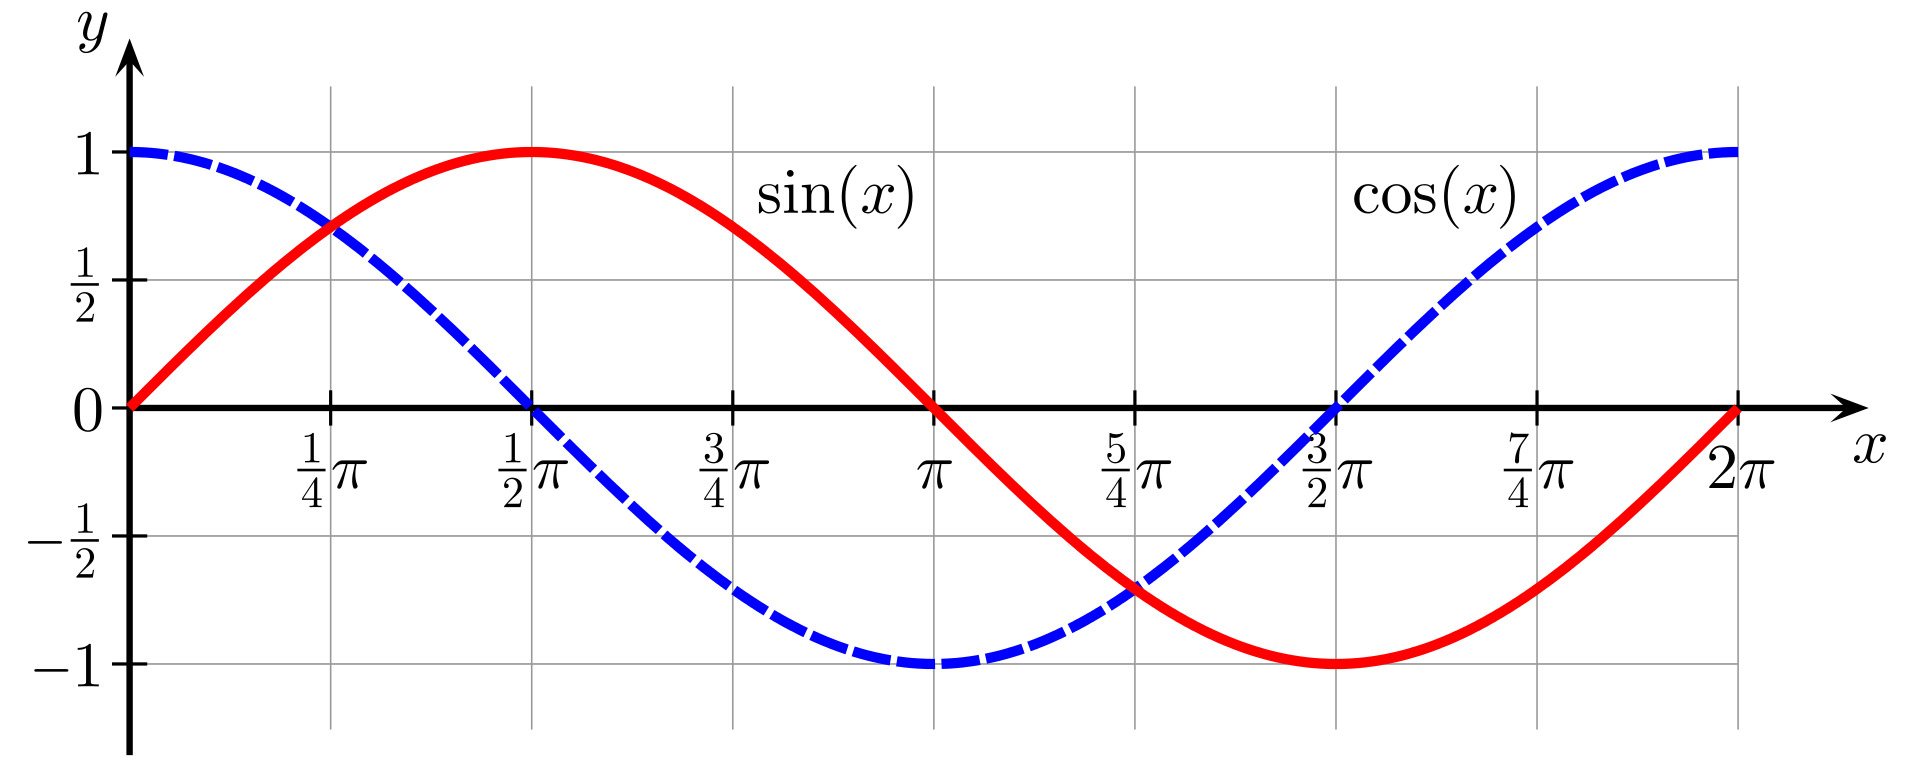
\includegraphics[scale=0.15]{sections/pics/Sine_cosine_one_period}
\end{center}

\subsubsection*{Anwendungsbeispiel B}
$\int \limits_1^e \frac{1}{x} \td{x}
= \ln(x) \bigg|_1^e = \ln(e) - \ln(1) = 1$. 

\subsubsection*{Anwendungsbeispiel C}
Nun interessieren wir uns für die die Integration von abschnittsweise definierten Funktionen, dass heißt:
\begin{align*}
f:[x_0,x_k] \to \mathbb{R}, \quad
f(x)
= 
\begin{cases}
g_1(x) &, \text{ für } x_0 \leq x < x_1 \\
g_2(x) &, \text{ für } x_1 \leq x < x_2\\
\vdots  &\ \\
g_k(x) &,  \text{ für } x_{k-1} \leq x < x_k
\end{cases}
\end{align*}
Funktionen dieser Art integrieren wir mit Eigenschaft 1 abschnittsweise:
\begin{align*}
\int \limits_{x_0}^{x_k} f(x) \td{x}
= \sum \limits_{i=1}^k \int \limits_{x_{i-1}}^{x_i} g_i(x) \td{x}
\end{align*}
Dieses Beispiel ist zunächst abstrakt.
Wir betrachten die Betragsfunktion
\begin{align*}
| \cdot | : \mathbb{R} \to [0,\infty) 
, \quad
x \mapsto 
\begin{cases}
x, &\ \text{falls } x \geq 0\\
-x, &\ \text{falls }  x < 0
\end{cases}.
\end{align*}
Hierbei symbolisiert $|\cdot |$ das Einsetzen von $x$-Werten für den Punkt.
Dann gilt:
\begin{align*}
\int \limits_{-1}^1 |x| \td{x}
&= \int \limits_{-1}^0 |x| \td{x}
+ \int \limits_{0}^1 |x| \td{x}
=\int \limits_{-1}^0 -x \td{x}
+ \int \limits_{0}^1 x \td{x}\\
&=
- \frac{1}{2} x^2 \bigg|_{-1}^0 + \frac{1}{2} x^2 \bigg|_{0}^1
=
-\left(\frac{1}{2} \cdot 0^2 - \frac{1}{2} \cdot  (-1)^2 \right)
+
\frac{1}{2} \cdot 1^2 - \frac{1}{2} \cdot 0^2
= \frac{1}{2} + \frac{1}{2} = 1
\end{align*}


\newpage

\subsection{Partielle Integration}
Die partielle Integration findet Anwendung, wenn
wir die zu integrierende Funktion als Produkt schreiben können.
Hierzu betrachten wir die Produktregel der Differenzialrechnung
\begin{align*}
(u(x) \cdot v(x))^\prime = u^\prime(x) v(x) + u(x) v^\prime(x)
\end{align*}
und wenden auf beiden Seiten das unbestimmte Integral an.
Dadurch erhalten wir mit
\begin{align*}
\textcolor{blue}{\int (u(x) \cdot v(x))^\prime \td{x}}
&=
\textcolor{green}{\int u^\prime(x) v(x) \td{x}} 
 + 
 \textcolor{red}{\int u(x) v^\prime(x)\td{x}}
 \\
\Leftrightarrow
\textcolor{green}{\int u^\prime(x) v(x) \td{x}}  &= \textcolor{blue}{\int (u(x) \cdot v(x))^\prime \td{x}} - \textcolor{red}{\int u(x) v^\prime(x)\td{x}}
= u(x) \cdot v(x) - \int u(x) v^\prime(x)\td{x}
\end{align*}
eine Rechenvorschrift zum Berechnen von Funktionen der Form $f(x) = u^\prime(x) v(x)$.
Die gleichen Rechnungen lassen sich auch mit bestimmten Integralen wiederholen.\\
\index{Integral!partielle Integration}
\begin{mybox}{Partielle Integration}
Seien $u, v$ Funktionen.
Dann gilt:
\begin{enumerate}
\item
$\int u^\prime(x) \cdot v(x) \td{x} = u(x) \cdot v(x) - \int u(x) v^\prime(x)\td{x} $
\item
$\int \limits_a^b u^\prime(x) \cdot v(x) \td{x} = u(x) \cdot v(x) \bigg|_a^b - \int \limits_a^b u(x) v^\prime(x)\td{x} $
\end{enumerate}
\end{mybox}
\ \\
Wir erkennen, dass diese Regel gleichermaßen für unbestimmte und bestimmte Integrale gilt.
Jedoch ist es häufig übersichtlicher zunächst die Stammfunktion mit partieller Integration zu bestimmen und dann den Hauptsatz anzuwenden.\\
\\
Durch partielle Integration lassen sich nun auch geschickt neue Stammfunktionen finden.
Wir betrachten 
\begin{align*}
\int \ln(x) \td{x} = 
\int\underbrace{ 1 \cdot \ln(x)v}_{u^\prime(x) \cdot v(x)}\td{x} 
= \underbrace{x \cdot \ln(x)}_{u(x) \cdot v(x)} - \int \underbrace{ x  \cdot \frac{1}{x}}_{u(x) \cdot v^\prime(x)} \td{x}= x \ln(x) -x + C
\end{align*}
mit $u^\prime(x) = 1 $ und $v(x) = \ln(x) $.
Nützlich ist die partielle Integration, wenn wir ein Produkt aus einer leicht integrierbaren Funktion und einer Funktion deren Ableitung nach endlichen vielen Ableitungen Null ergibt, haben.
Dies kann man sich an folgenden Integralen veranschaulichen:
\begin{align*}
&\int \limits_a^b x \cdot e^x \td{x}\\
&\int \limits_a^b x^{20} \sin(x) \td{x}\\
&\int \limits_a^b x^{1000} \cos(x) \td{x}
\end{align*}
Die erste Funktion ergibt Null nach endlich vielen Ableitungen.
Wir müssen nur lange genug Ableiten, damit die Funktion konstant wird.
Von den zweiten Funktionen kennen wir immer die Stammfunktion.
Die obigen Integrale lassen sich aus diesem Grund geschickt mit partieller Integration bestimmen, auch wenn wir die letzten beiden nicht von Hand ausrechnen wollen.

\subsubsection*{Anwendungsbeispiel}
Ein Investment Fonds generiert innerhalb der Zeitspanne von $t=0$ zu $T=12$ einen
stetigen Cashflow von $B(t) = 10 t + 5$.
Die Verzinsung erfolgt kontinuierlich zum Zinssatz $i = 5 \%$.
\\
\\
Bestimmen Sie den Nettobarwert $PV(0)$ zum Zeitpunkt $t = 0$ \textit{aller} Zahlungsströme,
die der Investment Fonds zwischen den Zeitpunkten $t = 0$ und $T = 12$ generiert.\\
\\
\textbf{Lösung:}
\begin{mdframed}
\underline{\textbf{Vorgehensweise:}}
\begin{enumerate}
\item Formuliere das Problem mathematisch.
\item Bestimme die nötige Stammfunktion mithilfe partieller Integration.
\item Berechne den Wert des Integrals.
\end{enumerate}
\end{mdframed}

\underline{1. Formuliere das Problem mathematisch}\\
Um den Nettobarwert $PV(0)$ zu bestimmen, müssen wir das Integral
\begin{equation*}
PV(0)
=
\int \limits_0^T B(t) e^{-i t} \ dt
=
\int \limits_0^{12} (10 t + 5) e^{-0.05 t} \ dt
\end{equation*}
berechnen.\\
\\
\underline{2. Bestimme die nötige Stammfunktion mithilfe partieller Integration}\\
%Zunächst betrachten wir die Produktregel und formen diese durch
%\begin{equation*}
%(u(t) v(t))^\prime = u^\prime(t) \cdot v(t) + u(t) \cdot v^\prime(t)
%\Leftrightarrow
%u(t) v^\prime(t) = (u(t)  v(t))^\prime - u^\prime(t) v(t)
%\end{equation*}
%um. Nun erhalten wir mit
%\begin{equation*}
%\int u(t) v^\prime(t) \ dt 
%= 
%\int (u(t)  v(t))^\prime \ dt - \int u^\prime(t) v(t) \ dt
%=
%u(t) v(t) - \int u^\prime(t) v(t) \ dt
%\end{equation*}
%die Regel für partielle Integration für unbestimmte Integrale.
%Für bestimmte Integrale geht die Umformung genauso.
%Dies war eine kurze Herleitung der partiellen Integration.
%Nun wenden wir diese Regel an.
Wir nutzen die Regel der partiellen Integration
\begin{align*}
\int u^\prime(t) \cdot v(t) \td{t} = u(t) \cdot v(t) - \int u(t) v^\prime(t)\td{t}
\end{align*}
und wählen hierfür
\begin{equation*}
\begin{split}
u^\prime(t)  =  e^{-0.05 t},  \quad
v(t)  = 10 t +5.
\end{split}
\end{equation*}
%für die partielle Integration.
Dies macht Sinn, denn $v$ wird nach einmal Ableiten konstant.
Es gilt 
\begin{equation*}
\begin{split}
u(t) = \frac{1}{-0.05} e^{-0.05t} 
=- \frac{100}{5} e^{-0.05t} = -20 e^{-0.05t}, \quad
v^\prime(t) = 10.
\end{split}
\end{equation*}
Mithilfe der Regel für partielle Integration erhalten wir
\begin{equation*}
\begin{split}
\int e^{-0.05 t} (10 t + 5)  \ dt
&= 
  -20  e^{-0.05 t} (10t +5)  - \int   -20 e^{-0.05t} \cdot 10  \ dt\\
&= -( 200 t + 100) e^{-0.05 t} + 200 \int e^{-0.05 t} \ dt\\
&=-(200 t + 100)  e^{-0.05t } + 200 (-20) e^{-0.05 t}  + C\\
&= -(200 t + 100) e^{-0.05 t } -4000 e^{-0.05t} + C \\
&= -(200 t +4100) e^{-0.05 t} + C
\end{split}
\end{equation*}
als Stammfunktion.\\

\newpage
\underline{3. Berechne den Wert des Integrals}\\
Da wir nun die Stammfunktion kennen, können wir das Integral direkt durch
\begin{align*}
\int \limits_0^{12} (10t + 5) e^{-0.05 t} \ dt
&=  \left[ -(200 t +4100) e^{-0.05 t} \right]_0^{12}\\
&= -(200 \cdot 12 +4100) e^{-0.05 \cdot 12} - (-(200 \cdot 0 +4100) e^{-0.05 \cdot 0} ) 
= -6500 e^{-0.6 }+4100 
\approx 532.70
\end{align*}
berechnen.\\
\\
Der Nettobarwert beträgt ungefähr $532.70$.

\newpage
\subsection{Integration durch Substitution}
\index{Integral!Substitution}
\begin{mybox}{Substitutionsregel}
Sei $f$ stetig und $g$ stetig differenzierbar.
Dann gilt:
\begin{align*}
\int \limits_a^b f( g(x)) \cdot g^\prime(x) \td{x} = 
\int \limits_{g(a)}^{g(b)} f(t) \td{t}
\end{align*}
Die Formel gilt analog für uneigentliche Integrale, nur eben ohne Grenzen.
\end{mybox}
Wir sehen bereits, dass $t = g(x) $ gelten muss.
Aber es ist noch nicht klar, wie $g^\prime(x)$ auf der rechten Seite verschwindet.
Hierfür schauen wir uns Folgendes an:
\begin{align*}
t = g(x) 
\Rightarrow
\frac{\mathrm{d} t}{\mathrm{d} x} = g^\prime(x) 
&\Leftrightarrow
\mathrm{d} t = g^\prime(x) \cdot \mathrm{d} x\\
&\Leftrightarrow
\mathrm{d} x = \frac{1}{g^\prime(x) } \cdot \mathrm{d} t
\end{align*}
Diese Umformungen geben uns zwei gleichwertige Möglichkeiten, die Substitution durchzuführen.
Die Erste ist $g^\prime(x)  \td{x} $ durch $\mathrm{d} t$ zu ersetzen.
Die Zweite ist, $\mathrm{d} x$ durch $\frac{1}{g^\prime(x) } \ \mathrm{d} t$ zu ersetzen.
Dadurch kürzt sich der $g^\prime(x)$ Term raus.\\ \\
Am einfachsten ist es die Substitution an Anwendungsaufgaben zu verstehen.
\newpage
\subsubsection*{Anwendungsbeispiel A}
Wir betrachten das Integral
\begin{align*}
\int \frac{2 x}{x^2} \td{x}
= 
\int \frac{1}{x^2} \cdot  2x \td{x}.
\end{align*}
Dann ist $f(x) = \frac{1}{x}$ und $g(x)=x^2$.
Wir können also 
\begin{align*}
\int \frac{1}{x^2} \cdot  2x \td{x} 
= 
\int f(g(x)) \cdot g^\prime(x)  \td{x}
\end{align*}
schreiben.
Wegen
\begin{align*}
t = g(x) = x^2 
\Rightarrow
\frac{\mathrm{d} t }{\mathrm{d} x}
= 
2 x 
\Leftrightarrow
\mathrm{d} t = 2x \ \mathrm{d} x
\end{align*}
können wir durch
\begin{align*}
\int \frac{1}{x^2} \cdot  2x \td{x}  = \int \frac{1}{t}  \td{t}  = \ln(t) +C =\ln(x^2) + C
\end{align*}
die Stammfunktion angeben.\\ \\
\textit{Wichtig:} Im letzten Schritt wurde rücksubstituiert.
Dies ist beim Berechnen von unbestimmten Integralen notwendig.
Bei bestimmten Integralen müssen wir dies nicht mehr machen.\\
Wir betrachten noch das ähnliche Integral
\begin{align*}
\int \frac{x}{x^2} \td{x} = \int \frac{1}{x^2} \cdot x \td{x}.
\end{align*}
Uns fällt auf, dass dieses Integral nicht die Form
\begin{align*}
\int f(g(x)) \cdot g^\prime(x)  \td{x}
\end{align*}
besitzt.
Zum Glück ist dies kein Problem.
Wir substituieren $t = x^2$.
Dann gilt wieder:
\begin{align*}
\frac{\mathrm{d} t }{\mathrm{d} x} = 2x 
\Leftrightarrow
\mathrm{d } x = \frac{1}{2 x} \td{t } = \frac{1}{2} \cdot \frac{1}{x} \td{t}
\end{align*}
Die weitere Rechnung werden wir nun so ausführlich wie möglich durchführen:
\begin{align*}
\int \frac{1}{x^2} \cdot x \td{x}
\stackrel{t = x^2}{=}
\int \frac{1}{t} \cdot x \td{x}
\stackrel{\mathrm{d } x = \frac{1}{2 x} \td{t }}{=}
\int \frac{1}{t} \cdot x \cdot \frac{1}{2x} \td{t}
= 
\frac{ 1}{2 } \cdot \int   \frac{1}{t} \td{t}
= 
\frac{1}{2} \cdot \ln(t) + C 
= 
\frac{1}{2} \cdot \ln(x^2) + C
\end{align*}
Was fällt uns auf?
Nach unserer Substitution hatten wir noch ein störendes $x$ im Integral.
Dieses kürzt sich jedoch mit $\mathrm{d} x = \frac{1}{2x} \mathrm{d}t$ heraus.
Der konstante Faktor interessiert uns beim Integrieren nicht. 
\newpage
\subsubsection*{Anwendungsbeispiel B}
Wir betrachten das bestimmte Integral
\begin{align*}
\int \limits_0^\pi \sin(\cos(x)) \cdot \sin(x) \td{x}.
\end{align*}

Wir substituieren $t = \cos(x)$.
Wegen
\begin{align*}
\frac{\mathrm{d} t}{\mathrm{d} x} = - \sin(x) 
\Leftrightarrow
\mathrm{d} x = -\frac{1}{\sin(x)} \td{t}
\end{align*}
erhalten wir 
\begin{align*}
\int \limits_0^\pi \sin(\cos(x)) \cdot \sin(x) \td{x}
= 
\int \limits_{\cos(0)}^{\cos(\pi)} \sin(t) \cdot \sin(x) \cdot \frac{-1}{\sin(x)} \td{t}
=
- \int \limits_{\cos(0)}^{\cos(\pi)} \sin(t)\td{t}
\end{align*}
als Integral. Bei bestimmten Integralen ist es notwendig, die Grenzen auch zu substituieren.
Mit 
\begin{align*}
\int \limits_0^\pi \sin(\cos(x)) \cdot \sin(x) \td{x}
&\stackrel{t = \cos(x)}{=}
- \int \limits_{\cos(0)}^{\cos(\pi)} \sin(t)\td{t}
=
- \int \limits_{1}^{-1} \sin(t)\td{t}
=
\int \limits_{-1}^{1} \sin(t)\td{t} \\ 
=
- \cos(t) \bigg|_{-1}^1 &= -\cos(1) + \cos(-1)
\stackrel{\text{a-symm.}}{=} -\cos(1) + \cos(1) = 0 
\end{align*}
erhalten wir den Wert des Integrals.
Hierbei haben wir die Achsensymmetrie der Kosinusfunktion verwendet.

\subsubsection*{Anwendungsbeispiel C}
Wir betrachten das Integral
\begin{align*}
\int \frac{f^\prime(x)}{f(x)} \td{x}.
\end{align*}
Mit $t = f(x) $ gilt
\begin{align*}
\frac{\mathrm{d} t}{\mathrm{d} x} = f^\prime(x)
\Leftrightarrow
\mathrm{d} t = f^\prime(x) \td{x}.
\end{align*}
Damit erhalten wir durch
\begin{align*}
 \int \frac{f^\prime(x)}{f(x)} \td{x}
 = 
 \int \frac{1}{t} \td{t} 
 =
 \ln(t) + C 
 =
 \ln(f(x)) + C
\end{align*}
eine allgemeine Stammfunktion für Funktionen der Form $\frac{f^\prime(x) }{f(x)}$.
Dies kann man direkt anwenden:
\begin{align*}
\int \frac{\cos(x)}{\sin(x)} \td{x} &= \ln(\sin(x)) +C \\
\int \frac{x}{ x^2} \td{x} &= \frac{1}{2} \int \frac{2x}{ x^2} \td{x} = \frac{1}{2} \ln(x^2) + C
\end{align*}

\newpage

\subsubsection*{Anwendungsbeispiel D}
Berechnen Sie das unbestimmte Integral
\begin{equation*}
\int \frac{\sin(\ln(x)) \ \cos(\ln(x))}{x} dx.
\end{equation*}
\textbf{Lösung:}
\begin{mdframed}
\underline{\textbf{Vorgehensweise:}}
\begin{enumerate}
\item Finde eine geeignete Substitution und bestimme die Stammfunktion.
\end{enumerate}
\end{mdframed}

\underline{1. Finde eine geeignete Substitution und bestimme die Stammfunktion}\\
Es gilt
\begin{equation*}
\frac{\text{d}}{\text{d} x}
\sin(\ln(x))
= \frac{\cos(\ln(x))}{x}
\end{equation*}
mit der Kettenregel.
Demnach haben wir durch
\begin{equation*}
\int \frac{\sin(\ln(x)) \ \cos(\ln(x))}{x} dx
=
\int \sin(\ln(x)) \cdot \frac{ \ \cos(\ln(x))}{x} dx
=
\int \sin(\ln(x)) \ \frac{\text{d}}{\text{d} x} \sin(\ln(x)) dx
\end{equation*}
die geeignete Substitution 
\begin{equation*}
u = \sin(\ln(x))
\end{equation*}
gefunden.
Durch 
\begin{equation*}
\frac{\text{d} u }{\text{d} x} = \frac{\cos(\ln(x))}{x}
\Rightarrow
\text{d}  u =  \frac{\cos(\ln(x))}{x} \ \text{d} x  
\end{equation*}
erhalten wir mit
\begin{equation*}
\int \frac{\sin(\ln(x)) \ \cos(\ln(x))}{x} dx 
=
\int u \ du
= \frac{1}{2} u^2 + C
= \frac{1}{2} (\sin(\ln(x)))^2 + C
\end{equation*}
die gesuchte Stammfunktion.\\ \\
Eine andere Möglichkeit ist, zweimal zu substituieren.
Zuerst substituieren wir $v = \ln(x)$.
Mit 
\begin{equation*}
\frac{\text{d} v}{\text{d} x}
= \frac{1}{x}
\Rightarrow
\text{d} v = \frac{1}{x} \ \text{d} x
\end{equation*}
erhalten wir
\begin{equation*}
\int \frac{\sin(\ln(x)) \ \cos(\ln(x))}{x} \ dx
= \int \sin(v) \cos(v) \ dv.
\end{equation*}
Die zweite Substitution ist $w = \sin(v)$.
Für diese gilt
\begin{equation*}
\frac{\text{d} w}{\text{d} v} = \cos(v)
\Rightarrow
\text{d} w = \cos(v) \ \text{d} v
\end{equation*}
und es folgt
\begin{equation*}
\begin{split}
\int \frac{\sin(\ln(x)) \ \cos(\ln(x))}{x} \ dx
&= \int \sin(v) \cos(v) \ dv
= \int w \ dw\\
&= \frac{1}{2} w^2 + C
= \frac{1}{2} (\sin(v))^2
= \frac{1}{2} (\sin(\ln(x)))^2 +C
\end{split}
\end{equation*}
durch zweimaliges Zurücksubstituieren.\\
\\
Die gesuchte Stammfunktion ist
\begin{align*}
\frac{1}{2} (\sin(\ln(x)))^2 +C.
\end{align*}

\subsection{Uneigentliches Integral}
Bisher haben wir nur Integrale von Funktionen betrachtet, welche auf beschränkten Intervallen definiert sind.
Doch wie sieht es aus, wenn Definitionslücken innerhalb der Integrationsgrenzen liegen oder die Grenzen $\pm \infty$ sind?
Wir können dies durch Grenzwerte auf bestimmte Integrale zurückführen.\\
\index{Integral!uneigentlich}
\begin{mybox}{Definition}
\begin{enumerate}
\item
Sei $f$ eine Funktion mit Definitionsbereich $D_f = [a,\infty)$, $D_f = (-\infty,b]$ oder $D_f = (-\infty, \infty)$.
Dann nennen wir 
\begin{align*}
\int\limits_a^\infty f(x) \td{x} &:= \lim  \limits_{\beta \to \infty} \int\limits_a^\beta f(x) \td{x}\\
\int\limits_{-\infty}^b f(x) \td{x} &:= \lim \limits_{\alpha \to \infty} \int\limits_{-\alpha}^b f(x) \td{x}\\
\int\limits_{-\infty}^{\infty} f(x) \td{x} &:=\lim \limits_{\alpha,\beta \to \infty} \int\limits_{-\alpha}^\beta f(x) \td{x}
\end{align*}
\textit{uneigentliche Integrale}, falls diese Grenzwerte existieren. 
\item
Sei $f$ eine Funktion mit Definitionslücke an der Stelle $b$.
Dann nennen wir
\begin{align*}
\int \limits_a^b f(x) \td{x} := \lim \limits_{\beta \to b} \int \limits_a^\beta f(x) \td{x} 
\end{align*}
\textit{uneigentliches Integral}, falls der Grenzwert existiert.
\end{enumerate}
\end{mybox}
Im Endeffekt läuft es darauf hinaus, dass wir wie gewohnt Stammfunktionen finden.
Wir müssen nur $\pm \infty$ Grenzen und Definitionslücken als Grenzwerte betrachten und überprüfen, ob diese Grenzwerte existieren.
\subsubsection*{Anwendungsbeispiel A}
Wir betrachten das Integral
\begin{align*}
\int \limits_0^1 \frac{1}{x^2} \td{x}.
\end{align*}
Warum ist dies uneigentlich? Die $0$ ist eine Definitionslücke von $\frac{1}{x^2}$.
Zunächst integrieren wir 
\begin{align*}
\int \limits_\alpha^1 \frac{1}{x^2} \td{x} = - \frac{1}{x} \bigg|_\alpha^1 =  -1 - \frac{-1}{\alpha}= -1 + \frac{1}{\alpha}
\end{align*}
mit $\alpha > 0$.
Wichtig ist hier, dass man nicht über die Definitionslücke laufen darf.
Nun gilt
\begin{align*}
\lim \limits_{\alpha \to 0}  \int \limits_\alpha^1 \frac{1}{x^2} \td{x}  = \lim \limits_{\alpha \to 0}  -1 + \frac{1}{\alpha} = \infty,
\end{align*}
womit der Grenzwert nicht existiert.
Damit ist 
\begin{align*}
\int \limits_0^1 \frac{1}{x^2} \td{x}.
\end{align*}
kein uneigentliches Integral.

\subsubsection*{Anwendungsbeispiel B}
Wir betrachten
\begin{align*}
\int \limits_1^\infty \frac{1}{x^2} \td{x}.
\end{align*}

Zunächst gilt
\begin{align*}
\int \limits_1^\beta \frac{1}{x^2} \td{x} = \frac{-1}{x} \bigg|_1^\beta = - \frac{1}{\beta} - (-1)
=
-\frac{1}{\beta } + 1
\end{align*}
womit wir durch
\begin{align*}
\lim \limits_{\beta \to \infty}  \int \limits_1^\beta \frac{1}{x^2} \td{x} 
= 
\lim \limits_{\beta \to \infty} - \frac{1}{\beta} + 1 = 1
\end{align*}
ein uneigentliches Integral gefunden haben.

\newpage
\subsection{Dichtefunktion}
\index{Dichtefunktion}
\begin{mybox}{Definition}
\index{Dichtefunktion}
Wir nennen eine Funktion $f$ \textit{Dichtefunktion} auf $I = [a,b] \subseteq \mathbb{R}$, falls
\renewcommand{\labelenumi}{(\roman{enumi})}
\begin{enumerate}
\item $f(x) \geq 0 $ für $x \in I$ 
\item $\int_I f(x) \td{x} =\int \limits_a^b f(x) \td{x}= 1$.
\end{enumerate}
erfüllt ist.
\end{mybox}

\subsubsection*{Anwendungsbeispiel A}
Die Funktion $f$ hat folgende Eigenschaften:
\renewcommand{\labelenumi}{(\roman{enumi})}
\begin{enumerate}
\item $f(x) \geq -3 $ für $x \in [0,1],$ und
\item $\int_0^1 f(x) dx = 3$.
\end{enumerate}
Dann gilt:
\renewcommand{\labelenumi}{(\alph{enumi})}
\begin{enumerate}
\item $g_1  =  \frac{1}{3} f $ ist eine Dichtefunktion auf $[0,1]$.
\item $g_2  =   f +3 $ ist eine Dichtefunktion auf $[0,1]$.
\item
$g_3  =  \frac{1}{6} f +3 $ ist eine Dichtefunktion auf $[0,1]$.
\item
$g_4  =  \frac{1}{6} f + \frac{1}{2} $ ist eine Dichtefunktion auf $[0,1]$.
\end{enumerate}
\ \\
Wir wissen, dass
\begin{align*}
g_1(x) = \frac{1}{3} f(x) \geq \frac{1}{3} (-3) = -1
\end{align*}
gilt.
Damit ist Antwort (a) falsch.\\
Für $g_2$ ist
\begin{align*}
g_2(x) = f(x) + 3 \geq -3 +3 = 0
\end{align*}
erfüllt. Jedoch ist die zweite Bedingung wegen
\begin{align*}
\int \limits_0^1 g_2(x) \ dx 
= 
\int \limits_0^1 f(x) + 3 \ dx
=
\int \limits_0^1 f(x) \ dx + \int \limits_0^1 3 \ dx
=
3 + 3 = 6
\end{align*}
nicht erfüllt.\\
Für $g_3$ ist wegen 
\begin{align*}
g_3(x) = \frac{1}{6} f + 3 \geq \frac{1}{6} \cdot (-3) +3
= -\frac{1}{2} +3 = \frac{5}{2}
\end{align*}
die erste Bedingung erfüllt.
Jedoch gilt
\begin{align*}
\int \limits_0^1 g_3(x) \ dx
= 
\frac{1}{6} \int \limits_0^1 f(x) \ dx + \int \limits_0^1 3 \ dx
= 
\frac{1}{6} \cdot 3 +  3 = \frac{1}{2} + 3 = \frac{7}{2}
\end{align*}
für die zweite Bedingung.
Also wissen wir schon durch das Ausschlußprinzip, dass Antwort (d) korrekt ist.
Die Funktion $g_4$ erfüllt beide Bedingungen:
\begin{align*}
g_4(x) &= \frac{1}{6} f(x) + \frac{1}{2}
= - \frac{1}{2} + \frac{1}{2} = 0\\
\int \limits_0^1 g_4(x) \ dx &=
\frac{1}{6} \int \limits_0^1 f(x) \ dx + \int \limits_0^1 \frac{1}{2} \ dx
= \frac{1}{2} + \frac{1}{2} = 1
\end{align*}
\ \\
Die Antwort (d) ist korrekt.

\newpage
\section{Differenzialrechnung}
Im Kapitel Differenzialrechnung werden wir die Themengebiete Extremwerte mit zwei Variablen, Extremwerte unter Nebenbedingungen betrachten und das Thema Homogenität wiederholen.
\subsection{Extremwertprobleme mit zwei Variablen}
Aus der eindimensionalen Differenzialrechnung wissen wir bereits,
dass
\begin{align*}
f^\prime(x) = 0
\end{align*}
als notwendige Bedingung für eine Extremstelle oder einen Sattelpunkt erfüllt sein muss.
Eine entsprechende Bedingung gibt es auch in der zweidimensionalen Differentialrechnung.\\
\index{stationäre Punkte!notwendiges Bed.}
\begin{mybox}{Notwendige Bedingung für stationäre Punkte}
Sei $f : \mathbb{R}^2 \to \mathbb{R}$ gegeben. 
Die \textit{notwendige Bedingung} für eine stationäre/kritische Stelle ist durch
\begin{align*}
f_x(x,y) &= 0\\
f_y(x,y) &= 0
\end{align*}
gegeben.
Alternativ können wir diese Bedingung auch als
\begin{align*}
\mathrm{grad} f (x,y) 
= 
\begin{pmatrix}
f_x(x,y)\\
f_y(x,y) 
\end{pmatrix}
= 
\textbf{0}
\end{align*}
schreiben.
\end{mybox}
Wir nennen dies einen stationären Punkt, da die Steigung Null beträgt.
Die Tangentialebene liegt also horizontal.
Hiermit können wir jedoch noch nicht mit Sicherheit sagen, ob es sich um ein Minimum,Maximum oder einen Sattelpunkt handelt.\\
\index{stationäre Punkte!hinreichende Bed.}
\begin{mybox}{Hinreichende Bedingungen}
Sei $f : \mathbb{R}^2 \to \mathbb{R}$ gegeben und $(x_0,y_0) $ ein kritischer Punkt.
Dann ist
\renewcommand{\labelenumi}{\theenumi.}
\begin{enumerate}
\item
\index{Minimum}
$f(x_0,y_0)$ ein \textit{Minimum}, falls
\begin{align*}
f_{xx}(x_0,y_0) > 0, \ f_{yy}(x_0,y_0) > 0, \ \text{und} \ f_{xx}(x_0,y_0)f_{yy}(x_0,y_0) - (f_{xy}(x_0,y_0))^2  > 0.
\end{align*}

\item
\index{Maximum}
$f(x_0,y_0)$ ein \textit{Maximum}, falls
\begin{align*}
f_{xx}(x_0,y_0) < 0, \ f_{yy}(x_0,y_0) < 0, \ \text{und} \ f_{xx}(x_0,y_0)f_{yy}(x_0,y_0) - (f_{xy}(x_0,y_0))^2  > 0.
\end{align*}

\item
\index{Sattelpunkt}
$f(x_0,y_0)$ ein \textit{Sattelpunkt}, falls
\begin{align*}
f_{xx}(x_0,y_0)f_{yy}(x_0,y_0) - (f_{xy}(x_0,y_0))^2  < 0.
\end{align*}

\end{enumerate}
\end{mybox}
\newpage




\pgfplotsset{width=7cm,compat=1.5.1}
\begin{tikzpicture}
\begin{axis}[view/h=10,view/v=20,axis lines = none]
\addplot3[
surf,
% shader=interp,
shader=flat,
samples=30,
domain=-3:3,y domain=-2:2]
{x^2 + y^2};
\end{axis}
\end{tikzpicture}
\begin{tikzpicture}
\begin{axis}[view/h=10,view/v=20,axis lines = none]
\addplot3[
surf,
% shader=interp,
shader=flat,
samples=30,
domain=-3:3,y domain=-2:2]
{-(x^2 + y^2)};
\end{axis}
\end{tikzpicture}
\begin{tikzpicture}
\begin{axis}[view/h=30,view/v=20,axis lines = none]
\addplot3[
surf,
% shader=interp,
shader=flat,
samples=30,
domain=-3:3,y domain=-2:2]
{x^2 -y^2};
\end{axis}
\end{tikzpicture}\\
Die Bilder veranschaulichen von links nach rechts:
Minimum, Maximum, Sattelpunkt.

\subsubsection*{Anwendungsbeispiel A}

Wir betrachten die Funktion $f(x,y) = x^2+ y^2 + 2y$.
Dann gilt
\begin{align*}
f_x(x,y) &= 2x\\
f_y(x,y) &= 2y+ 2
\end{align*}
für die partiellen Ableitungen.
Für stationäre Punkte muss die notwendige Bedingung 
\begin{align*}
f_x(x,y) &= 2x = 0 \ \Leftrightarrow \ x = 0\\
f_y(x,y) &= 2y +2 = 0 \ \Leftrightarrow \ 2y = -2 
\ \Leftrightarrow \ y = -1
\end{align*}
erfüllt sein.
Durch schnelles Nachrechnen sehen wir, dass $(0,-1)$ ein kritischer Punkt ist.
Für die Art des stationären Punktes benötigen wir noch die zweiten partiellen Ableitungen, welche durch
\begin{align*}
f_{xx}(x,y) &= 2\\
f_{yy}(x,y) &= 2\\
f_{xy}(x,y) &= 0
\end{align*}
gegeben sind.
Wir sehen, dass
\begin{align*}
f_{xx}(0,-1) > 0, \ f_{yy}(0,-1) > 0 , \ f_{xx}(0,-1) \cdot f_{yy}(0,-1) - (f_{xy}(0,-1))^2 > 0
\end{align*}
erfüllt ist.
Damit is unser stationärer Punkt $(0,-1)$ ein Minimum.
\newpage
\subsubsection*{Anwendungsbeispiel B}
Sei $f \ : \ \mathbb{R} \times (-5, \infty) \to \mathbb{R}$ eine Funktion zweier reeller Variablen definiert durch:
\begin{equation*}
f(x,y)\ = \ x^2 + 3 x y + 16 \ln(y+5).
\end{equation*}
Sei $g \ : \ R_f \to \mathbb{R}$ eine stetig differenzierbare Funktion einer reellen Variablen mit $g^\prime(x) > 0$
für alle $x \in R_f$, wobei $R_f$ der Wertebereich von $f$ ist.
Schließlich sei die Komposition $h$ gegeben als
\begin{equation*}
h \ : \ D_f \to \mathbb{R}, \quad (x,y) \mapsto h(x,y) = g(f(x,y)),
\end{equation*}
$D_f$ ist dabei das Definitionsgebiet von $f$.
\\
\\
Untersuchen Sie die Funktion $h$ auf stationäre Punkte, d.h., Maxima, Minima und Sattelpunkte.
\\
\\
\textbf{Hinweis:} \\
Dank der Eigenschaft von $g$ ist es möglich, das Problem in handhabbare Form zu bringen.\\

\textbf{Lösung:}
\begin{mdframed}
\underline{\textbf{Vorgehensweise:}}
\renewcommand{\labelenumi}{\theenumi.}
\begin{enumerate}
\item Verwende die gegebenen Eigenschaften, um das Problem zu strukturieren.
\item Finde die stationären Punkte von $h$.
\item Bestimme die Art des stationären Punkts.
\end{enumerate}
\end{mdframed}

\underline{1. Verwende die gegebenen Eigenschaften, um das Problem zu strukturieren}\\
Nach Voraussetzung ist $g^\prime(x) > 0$ für alle $x \in R_f$.
Die \textit{notwendige} Bedingung für stationäre Punkte ist, dass die partiellen Ableitungen von $h$ gleichzeitig Null sind.
Mathematisch können wir dies durch
\begin{align*}
h_x(x, y) = 0 \qquad 
h_y(x, y) = 0
\end{align*}
ausdrücken.
Die Punkte $(x, y)$, welche diese Bedingung erfüllen, nennen wir stationäre Punkte.
Wegen $g^\prime(x) > 0 $ gilt
\begin{align*}
h_x(x, y) &=  g^\prime(f(x,y)) \cdot f_x(x,y) = 0
\Leftrightarrow
f_x(x,y) = 0\\
h_y(x,y) &= g^\prime(f(x,y)) \cdot f_y(x,y) = 0 
\Leftrightarrow
f_y(x,y) = 0.
\end{align*}
Dies kann man sich mithilfe der Kettenregel überlegen.
Die Kettenregel findet Anwendung bei verketteten Funktionen sprich, wenn eine Funktion eine äußere und eine innere Funktion hat.
Dies ist bei 
\begin{align*}
h(x,y) = g(f(x,y)) 
\end{align*}
gegeben. Hierbei ist $g$ die äußere und $f$ die innere Funktion.
Die Kettenregel funktioniert hier wie im eindimensionalen Fall.
Wenn wir partiell nach $x$ ableiten, behandeln wir $y$ als eine Konstante.
Damit genügt es die stationären Punkte von $f$ zu bestimmen, da diese mit denen von $h$ übereinstimmen.
Wegen $g^\prime(x) > 0 $ können $h_x$ und $h_y$ nur Null ergeben, wenn $f_x$ bzw. $f_y$ Null ergeben.\\
\newpage
\underline{2. Finde die stationären Punkte von $h$}\\
Zunächst bestimmen wir durch
\begin{equation*}
\begin{split}
f_x(x,y) &= 2x + 3y \\
f_y(x,y) &= 3x + 16 (y+5)^{-1} = 3x + \frac{16}{y+5}
\end{split}
\end{equation*}
die ersten partiellen Ableitungen von $f$.
Diese müssen nun die \textit{notwendigen} Bedingungen
\begin{equation*}
f_x(x,y) = 0 \ \text{und} \ f_y(x,y) = 0
\end{equation*}
erfüllen. Dies führt zu dem Gleichungssystem
\begin{equation*}
\begin{split}
f_x(x,y) &= 2x + 3y = 0\\
f_y(x,y) &=  3x + \frac{16}{y+5} = 0.
\end{split}
\end{equation*}
Durch Umformen der ersten Gleichung erhalten wir mit
\begin{equation*}
2x + 3y = 0 
\Leftrightarrow
3y = -2x
\Leftrightarrow
y = -\frac{2}{3} x 
\end{equation*}
eine Darstellung für $y$.
Wir lösen die Gleichung durch Einsetzen in die Mitternachtsformel:
\begin{equation*}
\begin{split}
&3x + \frac{16}{y+5} = 3x + \frac{16}{-\frac{2}{3}x+5} = 0\\
\Leftrightarrow
&3x \left( -\frac{2}{3}x+5 \right) + 16 = -2 x^2 + 15 x + 16 = 0\\
\Leftrightarrow
&x_{\nicefrac{1}{2}}= \frac{- 15 \pm \sqrt{15^2 - 4 \cdot (-2) \cdot 16}}{2 \cdot(- 2)} 
= \frac{15 \pm \sqrt{353}}{4}\\
\Rightarrow
&x_1 = \frac{15 - \sqrt{353}}{4}, \quad
x_2 = \frac{15 + \sqrt{353}}{4}
\end{split}
\end{equation*}
Wir setzen nun $x_1$ und $x_2$ in die Gleichung $y = -\frac{2}{3} x$ ein und bestimmen so die möglichen stationären Punkte:
\begin{equation*}
\begin{split}
x_1  = \frac{15 - \sqrt{353}}{4}
&\Rightarrow
y_1 = -\frac{2}{3} x_1 = \frac{-15 + \sqrt{353}}{6}
\Rightarrow
P_1 = \left( \frac{15 - \sqrt{353}}{4}, \frac{-15 + \sqrt{353}}{6} \right)
\\
x_2  = \frac{15 + \sqrt{353}}{4}
&\Rightarrow
y_2 = -\frac{2}{3} x_2 = \frac{-15 - \sqrt{353}}{6}
\Rightarrow
P_2 = \left( \frac{15 + \sqrt{353}}{4}, \frac{-15 - \sqrt{353}}{6} \right).
\end{split}
\end{equation*}
Wir können den Punkt $P_2$ direkt ausschließen, da dieser sich nicht in dem Definitionsgebiet von $f$ befindet.
Dies können wir an
\begin{align*}
\frac{-15 - \sqrt{353}}{6} < -5
\end{align*}
erkennen.
Unser stationärer Punkt ist also durch
\begin{align*}
P_1 = \left( \frac{15 - \sqrt{353}}{4}, \frac{-15 + \sqrt{353}}{6} \right)
\end{align*}
gegeben.\\

\newpage

\underline{3. Bestimme die Art des stationären Punkts}\\
Auch hier reicht es wieder $f$ zu untersuchen.
Zunächst betrachten wir die \textit{hinreichenden} Bedingungen für Maxima, Minima und Sattelpunkte.\\

\begin{mybox}{Hinreichende Bedingungen}
Sei $f : \mathbb{R}^2 \to \mathbb{R}$ gegeben und $(x_0,y_0) $ ein kritischer Punkt.
Dann ist
\renewcommand{\labelenumi}{\theenumi.}
\begin{enumerate}
\item
\index{Minimum}
$f(x_0,y_0)$ ein \textit{Minimum}, falls
\begin{align*}
f_{xx}(x_0,y_0) > 0, \ f_{yy}(x_0,y_0) > 0, \ \text{und} \ f_{xx}(x_0,y_0)f_{yy}(x_0,y_0) - (f_{xy}(x_0,y_0))^2  > 0.
\end{align*}

\item
\index{Maximum}
$f(x_0,y_0)$ ein \textit{Maximum}, falls
\begin{align*}
f_{xx}(x_0,y_0) < 0, \ f_{yy}(x_0,y_0) < 0, \ \text{und} \ f_{xx}(x_0,y_0)f_{yy}(x_0,y_0) - (f_{xy}(x_0,y_0))^2  > 0.
\end{align*}

\item
\index{Sattelpunkt}
$f(x_0,y_0)$ ein \textit{Sattelpunkt}, falls
\begin{align*}
f_{xx}(x_0,y_0)f_{yy}(x_0,y_0) - (f_{xy}(x_0,y_0))^2  < 0.
\end{align*}
\end{enumerate}
\end{mybox}
Wir bestimmen nun die zweiten partiellen Ableitungen von $f$.
Es gilt
\begin{equation*}
\begin{split}
f_{xx}(x,y)  &= 
\frac{\partial}{\partial \mathrm{x}} (2x + 3y) = 2
 \\
f_{xy}(x,y)  &=
= \frac{\partial}{\partial \mathrm{y}} (2x + 3y) 
= 3 \\
f_{yy}(x,y) &= 
\frac{\partial}{\partial \mathrm{y}} \left(3x + \frac{16}{y+5} \right)
=
\frac{\partial}{\partial \mathrm{y}} \left(3x + 16 \cdot (y+5)^{-1} \right)
= 16 \cdot (-1)\cdot(y+5)^{-2}
- \frac{16}{(y+5)^2}.
\end{split}
\end{equation*}
Wir sehen, dass $f_{xx}(x,y) > 0$ für alle $(x,y) \in D_f$ gilt. 
Es gilt auch $f_{yy}(x,y) < 0 $ für alle $(x,y) \in D_f$.
Damit ist 
\begin{equation*}
\underbrace{f_{xx}(x,y)}_{>0} \underbrace{f_{yy} (x,y)}_{< 0 } - \underbrace{(f_{xy}(x,y))^2}_{>0} < 0
\end{equation*}
für alle $(x,y) \in D_f$ gegeben.
Somit ist $P_1 $ ein Sattelpunkt.

\newpage


\subsection{Gradient}

\begin{mybox}{Definition}\index{Gradient}
Sei $f : \mathbb{R}^2 \to \mathbb{R}$ gegeben.
Dann ist der \textit{Gradient} durch
\begin{align*}
\mathrm{grad} f(\textbf{x}) = 
\mathrm{grad} f(x,y) :=
\begin{pmatrix}
f_x(x,y)\\
f_y(x,y)
\end{pmatrix}
\end{align*}
definiert.
Damit ist der Gradient der Vektor der partiellen Ableitungen.
\end{mybox}

\begin{figure}[H]
\centering
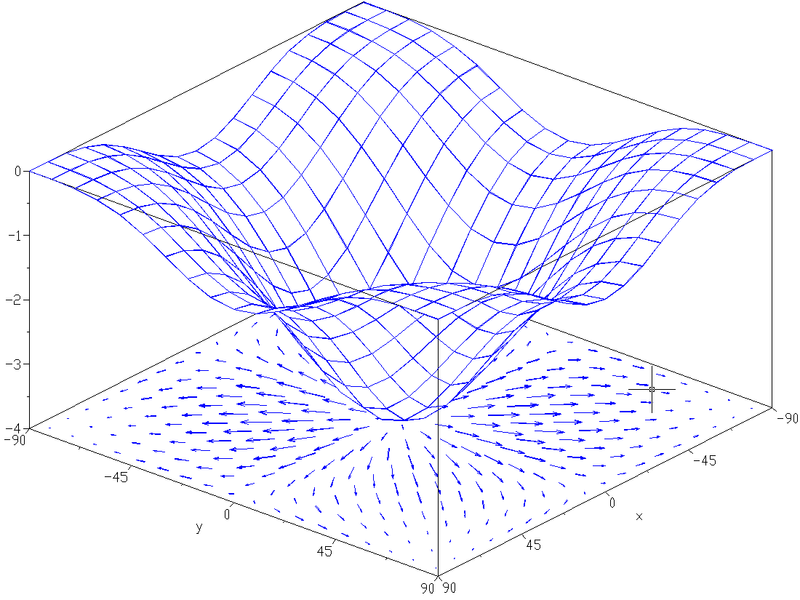
\includegraphics[scale=0.5]{sections/pics/gradient.png}
\end{figure}
Den Graph einer Funktion der Form $f : \mathbb{R}^2 \to \mathbb{R} $ können wir uns als ein Gebirge vorstellen. 
Der Gradient im Punkt $\textbf{x}$ liefert uns die Richtung des stärksten Anstiegs.
Die blauen Pfeile in der Ebene sind die Gradienten an den entsprechenden Punkten.
Wir wissen also mit dem Gradienten, in welche Richtung wir den \glqq Berg\grqq~am schnellsten besteigen können.
\\
\begin{mybox}{Wichtige Eigenschaft}
\begin{center}
$\mathrm{grad} f(x,y) = \ \text{\glqq Richtung des größten Anstiegs von $f$ in $(x,y)$\grqq}$
\end{center}
\end{mybox}
\subsubsection*{Anwendungsbeispiel A}
Sei $f(x,y) = -x^2 + 3 y^2 -5$. Dann gilt:
\begin{align*}
\mathrm{grad} f(x,y) = 
\begin{pmatrix}
f_x(x,y)\\
f_y(x,y)
\end{pmatrix}
= 
\begin{pmatrix}
-2x\\
6 y
\end{pmatrix}
\end{align*}
\newpage
\subsubsection*{Anwendungsbeispiel B}
Sei $f(x,y) = \sin(x) \cdot \cos(y)$.\\
Bestimmen Sie die Richtung des größten Anstiegs im Punkt $(0,\pi)$.\\
\\
Es gilt:
\begin{align*}
\mathrm{grad} f(x,y) = 
\begin{pmatrix}
f_x(x,y)\\
f_y(x,y)
\end{pmatrix}
=
\begin{pmatrix}
\cos(x) \cdot \cos(y)\\
-\sin(x) \cdot \sin(y)
\end{pmatrix}
\end{align*} 
Damit folgt:
\begin{align*}
\mathrm{grad} f(0,\pi)
=
\begin{pmatrix}
\cos(0) \cdot \cos(\pi)\\
-\sin(0) \cdot \sin(\pi)
\end{pmatrix}
=\begin{pmatrix}
1 \cdot (-1)\\
0 \cdot 0
\end{pmatrix}
=
\begin{pmatrix}
-1\\
0
\end{pmatrix}
\end{align*}
Damit ist $\begin{pmatrix} -1 & 0\end{pmatrix}^\top$ die Richtung des größten Anstiegs im Punkt $(0, \pi)$ von $f$.\\

\subsubsection*{Anwendungsbeispiel C}
Gegeben sei die Funktion zweier reeller Variablen 
$f \ : \ \mathbb{R}\times \mathbb{R} \to \mathbb{R}$ definiert durch:
\begin{equation*}
f(x,y) = e^{2x^2+y^3 +3x +3y}.
\end{equation*}
Bestimmen Sie die Gleichung (allgemeine Form) einer Ebene $\beta$ so,
dass der Vektor $\textbf{u} = (x_0,y_0,z_0)^\top$ orthogonal zu $\beta$ ist,
wobei $(x_0,y_0)^\top = \textbf{grad} f(0,0)$ und $z_0 = f(0,0)$ gilt.
\\
\\
\textbf{Lösung:}
\begin{mdframed}
\underline{\textbf{Vorgehensweise:}}
\renewcommand{\labelenumi}{\theenumi.}
\begin{enumerate}
\item Stelle eine passende Ebenengleichung auf und berechne die fehlenden Parameter.
\end{enumerate}
\end{mdframed}

\underline{1. Stelle eine passende Ebenengleichung auf und berechne die fehlenden Parameter}\\
Da der Vektor $\textbf{u} = (x_0,y_0,z_0)^\top$ orthogonal auf $\beta$ ist, ist $\textbf{u}$ ein Normalenvektor.
Damit können wir $\beta$ durch
\begin{align*}
\beta \ : \ x_0 x + y_0 y + z_0 z + d  = 0, \qquad d \in \mathbb{R}
\end{align*}
beschreiben.
Wir müssen also nur noch $\text{u}$ bestimmen.
Es gilt  
\begin{align*}
\textbf{grad} f(x,y) = e^{2x^2+y^3 +3x +3y} 
\begin{pmatrix}
4 x+ 3\\
3 y^2 + 3 
\end{pmatrix}
\end{align*}
für den Gradienten von $f$.
Durch
\begin{align*}
\textbf{grad} f(0 ,0)&=
e^0
\begin{pmatrix}
3\\
3
\end{pmatrix}
=
\begin{pmatrix}
3\\
3
\end{pmatrix} \\
f(0,0) &= e^0 = 1
\end{align*}
erhalten wir $(x_0,y_0,z_0)^\top = ( 3, 3,1)^\top$.
Damit haben wir durch
\begin{align*}
\beta \ : \ 3 x + 3 y + 1 z + d, \qquad d \in \mathbb{R}
\end{align*}
die allgemeine Form von $\beta$ gegeben.



\newpage
\subsection{Extremwerte unter Nebenbedingungen}
Wir haben eine Funktion mit $f : \mathbb{R}^2 \to \mathbb{R}$ gegeben.
Nun interessieren uns die Extrempunkte unter der Bedingung, dass 
\begin{align*}
\varphi(x,y) = 0
\end{align*}
erfüllt ist.
Dieses $\varphi$ nennen wir \textit{Nebenbedingung}.
Wichtig ist, dass die Nebenbedingung in der Aufgabenstellung beispielsweise durch
\begin{align*}
x = -y
\end{align*}
geben sein kann.
Durch die Umformung
\begin{align*}
x = -y 
\Leftrightarrow
\varphi(x,y) = x + y = 0
\end{align*}
erhalten wir dann die erforderliche Form.\\
\index{Substitutionsmethode}
\begin{mybox}{Substitutionsmethode}
Gegeben sei eine Funktion $f : \mathbb{R}^2 \to \mathbb{R}$ und
die Nebenbedingung $\varphi(x,y) = 0$.
Wenn es möglich ist, die Nebenbedingung durch
\begin{align*}
\varphi(x,y) = 0 \Leftrightarrow
y = g(x) 
\end{align*}
oder 
\begin{align*}
\varphi(x,y) = 0 \Leftrightarrow
x = g(y) 
\end{align*}
nach einer Variablen umzustellen, können wir das Extremwertproblem durch
Zurückführen auf die eindimensionale Differenzialrechnung lösen.
Durch Einsetzen von $y=g(x)$ erhalten wir mit
\begin{align*}
\tilde{f}(x) := f(x,y) = f(x,g(x))
\end{align*}
oder
\begin{align*}
\tilde{f}(y) := f(x,y) = f(g(y),y)
\end{align*}
das eindimensionale Extremwertproblem.
\end{mybox}
Dieses Verfahren nennen wir \textit{Substitutionsmethode}.
Da bei diesem Verfahren eine Variable verloren geht, wird ebenfalls der Name 
\textit{Variablenreduktion} oder \textit{Reduktionsmethode} verwendet.
Wann können wir dieses Verfahren anwenden?
Im Prinzip immer, wenn wir eindeutig nach einer Variablen auflösen können.\\ \\
Wir betrachten die Nebenbedingung
\begin{align*}
\varphi(x,y) = 2x -4y = 0.
\end{align*}
Diese lässt sich durch
\begin{align*}
2x - 4 y = 0 
\Leftrightarrow
x = 2y
\Leftrightarrow
y = \frac{1}{2} x
\end{align*}
eindeutig nach beiden Variablen umformen.
\newpage
Dies ist bei der Nebenbedingung
\begin{align*}
\varphi(x,y) = x^2 + y = 0
\end{align*}
nicht für beide Variablen möglich.
Durch 
\begin{align*}
y = -x^2 
\end{align*}
erhält man eine eindeutige Zuordnung für die $y $-Variable.
Jedoch ist wegen
\begin{align*}
x^2 + y = 0
\Leftrightarrow
x = \pm \sqrt{-y}
\end{align*}
keine eindeutige Zuordnung für die $x$-Variable möglich.\\

Da das Umformen nach einer Variablen nicht immer möglich ist, betrachten wir nun das \textit{Lagrange-Verfahren}.
\index{Lagrangeverfahren}
\begin{mybox}{Lagrangefunktion}
\index{Lagrangefunktion}
Geben sei eine Funktion $f : \mathbb{R}^2 \to \mathbb{R}$ und eine Nebenbedingung 
$\varphi(x,y) = 0$.
Dann bezeichnen wir 
\begin{align*}
F(x,y,\lambda) = f(x,y) + \lambda \varphi(x,y) 
\end{align*}
als \textit{Lagrangefunktion}.
\end{mybox}
\ \\
Doch wie finden wir nun mit dieser Funktion Extremwerte unter der Nebenbedingung?
Da dies eine mehrdimensionale Funktion ist, müssen auch alle partiellen Ableitungen gleichzeitig Null sein.\\

\begin{mybox}{Notwendige Bedingung für die Lagrangefunktion}
\index{Lagrangefunktion!notwendige Bed.}
Die notwendige Bedingung für Extremstellen unter der Nebenbedingung $\varphi(x,y) = 0$
ist durch
\begin{align*}
F_x(x,y,\lambda )&= 0\\
F_y(x,y,\lambda) &= 0\\
F_\lambda(x,y,\lambda) &= 0
\end{align*}
gegeben.
Die Punkte, welche diese Bedingung erfüllen, nennen wir wieder \textit{kritische/stationäre} Punkte.
\end{mybox}
\ \\
Wir können das Vorgehen hier in drei Schritte unterteilen:
\begin{mybox}{Vorgehensweise:}

Schritt 1: Aufstellen der Lagrangefunktion\\
Schritt 2: Bilden der ersten partiellen Ableitung nach $x$, $y$ und $\lambda$.\\
Schritt 3: Lösen des Gleichungssystem der notwendigen Bedingung für die Lagrangefunktion.

\end{mybox}
\newpage
\subsubsection*{Anwendungsbeispiel A}
Bestimmen Sie die Extrempunkte der Funktion
\begin{align*}
f(x,y) = x^2 +y^2
\end{align*}
unter der Nebenbedingung $\varphi(x,y) = x +4 y -2$.\\
\\
\underline{1. Aufstellen der Lagrangefunktion}\\
Die Lagrangefunktion ist durch
\begin{align*}
F(x,y,\lambda) = f(x,y) + \lambda \varphi(x,y) 
= x^2 +y^2 + \lambda(x +4 y -2).
\end{align*}
gegeben.\\
\\
\underline{2. Bilden der ersten partiellen Ableitung nach $x$, $y$ und $\lambda$}\\
Es gilt
\begin{align*}
F_x(x,y,\lambda) &= 2x + \lambda\\
F_y(x,y,\lambda) &= 2y + 4 \lambda\\
F_\lambda(x,y,\lambda) &= x+ 4y -2
\end{align*}
für die partiellen Ableitungen.\\
\\
\underline{3. Lösen des Gleichungssystem der notwendigen Bedingung für die Lagrangefunktion}\\
Nun gilt
\begin{align*}
F_x(x,y,\lambda) &= 2x + \lambda\ = 0 
\Leftrightarrow
\lambda = -2x\\
F_y(x,y,\lambda) &= 2y + 4 \lambda = 0
\Leftrightarrow 
\lambda = - \frac{1}{2}y\\
\Rightarrow
-2x &= - \frac{1}{2} y
\Leftrightarrow
y = 4 x,
\end{align*}
wodurch wir $\lambda$ eliminiert haben.
Setzen wir $y = 4x $ in die letzte Gleichung ein, erhalten wir durch
\begin{align*}
F_\lambda(x,y,\lambda) &= x +4y -2 = x + 16 x -2 = 0\\
\Leftrightarrow
x &= \frac{2}{17}
\Leftrightarrow
y = 4x = 4 \cdot \frac{2}{17} = \frac{8}{17} 
\end{align*}
den kritischen Punkt $\left( \frac{2}{17}, \frac{8}{17} \right)$.\\
\\
\begin{mybox}{Hinreichende Bedingung für Lagrangefuntion}
\index{Lagrangefunktion!hinreichende Bed.}
\renewcommand{\labelenumi}{\theenumi.}
\begin{enumerate}
\item
Falls
\begin{align*}
2 \varphi_x(x,y)\varphi_y(x,y) F_{xy}(x,y,\lambda)
-F_{xx}(x,y,\lambda) \varphi_y^2(x,y) 
- F_{yy}(x,y,\lambda)\varphi_x^2(x,y) < 0
\end{align*}
gilt, liegt ein \textit{Minimum} vor.
\item
Falls
\begin{align*}
2 \varphi_x(x,y)\varphi_y(x,y) F_{xy}(x,y,\lambda)
-F_{xx}(x,y,\lambda) \varphi_y^2(x,y) 
- F_{yy}(x,y,\lambda)\varphi_x^2(x,y) > 0
\end{align*}
gilt, liegt ein \textit{Maximum} vor.
\end{enumerate}
\end{mybox}

\subsubsection*{Fortsetzung des Anwendungsbeispiels A}
Zunächst bestimmen wir mit
\begin{align*}
\varphi_x(x,y) &= 1 \\
\varphi_y(x,y) &= 4\\
F_{xx}(x,y,\lambda) &= 2 \\
F_{yy}(x,y,\lambda) &= 2\\
F_{xy}(x,y,\lambda) &= 0
\end{align*}
die für die hinreichende Bedingung notwendigen Ableitungen.
Mit $(x,y) :=  \left( \frac{2}{17}, \frac{8}{17} \right)$ folgt dann durch
\begin{align*}
&2 \varphi_x(x,y)\varphi_y(x,y) F_{xy}(x,y,\lambda)
-F_{xx}(x,y,\lambda) \varphi_y^2(x,y) 
- F_{yy}(x,y,\lambda)\varphi_x^2(x,y)\\
=
&2 \cdot 1 \cdot 4 \cdot 0 - 2 \cdot 4^2 - 2 \cdot 1^2 
=
- 32 - 2 = -34 < 0,
\end{align*}
dass es sich bei dem Punkt $\left( \frac{2}{17}, \frac{8}{17} \right)$ um ein Minimum von $f$ unter der Nebenbedingung $\varphi$ handelt.\\
\\

\subsubsection*{Anwendungsbeispiel B}
Ein Konsument \textit{maximiert} seine Nutzenfunktion $u(c_1,c_2)$ in den Einheiten $c_1$ und $c_2$
der Güter 1 und 2 definiert durch:
\begin{equation*}
u \ : \ \mathbb{R}_+ \times \mathbb{R}_+ \to \mathbb{R},
\quad (c_1,c_2) \mapsto u(c_1,c_2) = c_1^{0.6} c_2^{0.4}
\end{equation*}
über die Wahl des Konsumbündels $(c_1^\star,c_2^\star)$.
Die Preise der Güter 1 und 2 sind $p_1 \ = \ 3$ beziehungsweise $p_2 \ = \ 4$,
und das Budget, welches \textit{vollständig} genutzt wird, beträgt $e = 15$.
\\
Bestimmen Sie die stationären Punkte des Maximierungsproblems des Konsumenten, 
d.h., Kandidaten für das optimale Konsumbündel $(c_1^\star,c_2^\star)$.
\\
\\
\textbf{Hinweis:}\\ 
Eine Abklärung, ob es sich bei den stationären Punkten tatsächlich um Maxima handelt, wird nicht verlangt.
\\
\\
\textbf{Lösung:}
\begin{mdframed}
\underline{\textbf{Vorgehensweise:}}
\renewcommand{\labelenumi}{\theenumi.}
\begin{enumerate}
\item Formuliere das Optimierungsproblem mathematisch.
\item Löse die Aufgabe mithilfe der Lagrange Methode.
\item Alternative Rechenmethode.
\end{enumerate}
\end{mdframed}
\underline{1. Formuliere das Optimierungsproblem mathematisch}\\
Unser Ziel ist es, die Funktion
\begin{equation*}
u(c_1,c_2) = c_1^{0.6}c_2^{0.4}
\end{equation*}
unter der Nebenbedingung
\begin{equation*}
p_1 c_1 + p_2 c_2 = e \Rightarrow
\varphi(c_1,c_2) = p_1 c_1 + p_2 c_2 - e = 3 c_1 + 4 c_2 - 15 = 0
\end{equation*}
zu maximieren.
\\
\\
\underline{2. Löse die Aufgabe mithilfe der Lagrange Methode}\\
Zunächst bietet es sich bei Extremwertaufgaben unter Nebenbedingungen an, die Lagrange Methode zu verwenden
Die Nebenbedingung
\begin{equation*}
\varphi(c_1,c_2) = 3 c_1 + 4 c_2 - 15 = 0
\end{equation*}
besitzt nur lineare Terme.
Das heißt, wir können diese explizit nach $c_1$ bzw. $c_2$ auflösen.
Durch diese Umformung erhalten wir aus $u$ eine Funktion, welche von einer Variablen abhängt.
Beide Methoden sind in etwa gleich schwer, jedoch funktioniert die zweite Methode nicht immer.
\\
\\ 
Wir definieren durch
\begin{equation*}
F(c_1,c_2,\lambda) = u(c_1,c_2) + \lambda \varphi(c_1,c_2)
= c_1^{0.6}c_2^{0.4} + \lambda \cdot( 3 c_1 + 4 c_2- 15)
\end{equation*}
die Lagrange-Funktion.
Die notwendige Bedingung für Extremstellen unter unserer Nebenbedingung ist,
dass die partiellen Ableitungen der Lagrange-Funktion gleichzeitig Null sind.
Durch
\begin{align*}
F_{c_1}(c_1,c_2,\lambda) &= 0.6 c_1^{-0.4} c_2^{0.4} + 3 \lambda\\
F_{c_2}(c_1,c_2, \lambda) &= 0.4 c_1^{0.6} c_2^{-0.6} + 4 \lambda \\
F_{\lambda}(c_1,c_2,\lambda) &=\varphi(c_1,c_2) = 3 c_1 + 4 c_2 -15 
\end{align*}
erhalten wir die partiellen Ableitungen.
Wir müssen nun das Gleichungssystem
\newcounter{eq}
\setcounter{eq}{0}
\begin{align}
0.6 c_1^{-0.4} c_2^{0.4} + 3 \lambda = 0  \tag{\text{\Roman{eq}}}\stepcounter{eq}\\
0.4 c_1^{0.6} c_2^{-0.6} + 4 \lambda = 0  \tag{\text{\Roman{eq}}}\stepcounter{eq}\\
3 c_1 + 4 c_2 -15 = 0 \tag{\text{\Roman{eq}}}\stepcounter{eq}
\end{align}
lösen. 
Die Gleichungen (I) und (II) liefern uns durch
\begin{align}
0.6 c_1^{-0.4} c_2^{0.4} + 3 \lambda &= 0 
\Leftrightarrow 
3 \lambda = -0.6 c_1^{-0.4} c_2^{0.4} 
\Leftrightarrow
3 \lambda= -0.6 \frac{c_2^ {0.4}}{c_1^{0.4}}
\Leftrightarrow
3 \lambda= -0.6 \left( \frac{c_2}{c_1} \right)^{0.4}
\tag{\text{\Roman{eq}}}\stepcounter{eq}\\
0.4 c_1^{0.6} c_2^{-0.6} + 4 \lambda &= 0 
\Leftrightarrow 
4 \lambda = - 0.4 c_1^{0.6} c_2^{-0.6} 
\Leftrightarrow
4 \lambda = -0.4  \frac{c_1^{0.6}}{c_2^{0.6}}
\Leftrightarrow
4 \lambda=- 0.4 \left( \frac{c_1}{c_2} \right)^{0.6}
\tag{\text{\Roman{eq}}}\stepcounter{eq}    
\end{align}
zwei neue Gleichungen.
Wegen $c_1, c_2 > 0 $ sehen wir, dass $\lambda \neq 0 $ gilt.
Also können wir (IV) durch (V) teilen.
Damit gilt
\begin{equation*}
\begin{split}
\frac{3 \lambda }{4 \lambda} 
&= \frac{-0.6 \left( \frac{c_2}{c_1} \right)^{0.4}}{- 0.4 \left( \frac{c_1}{c_2} \right)^{0.6}}
= \frac{3}{2} \cdot \frac{c_2^{0.4} c_2^{0.6}}{c_1^{0.6} c_1^{0.4}}
= \frac{3}{2} \frac{c_2}{c_1}\\
\Rightarrow
\frac{3 \lambda }{4 \lambda} &= \frac{3}{2} \frac{c_2}{c_1}
\Leftrightarrow
\frac{3  }{4 } = \frac{3}{2} \frac{c_2}{c_1}
\Leftrightarrow
6 c_1 = 12 c_2
\Leftrightarrow
c_1 = 2 c_2,
\end{split}
\end{equation*}
womit durch Gleichung (III)
\begin{equation*}
\begin{split}
3 c_1 + 4 c_2 - 15 &= 3 (2c_2) + 4 c_2 -15 = 10 c_2  -15 = 0 \\
\Leftrightarrow
10 c_2 &= 15 
\Leftrightarrow
c_2 = \frac{15}{10} = \frac{3}{2} = 1.5  
\end{split}
\end{equation*}
folgt.
Durch $c_1 = 2 c_2 $ wissen wir auch $c_1 = 3$.
Damit ist 
\begin{align*}
(c_1^\star, c_2^\star) = ( 3, 1.5)
\end{align*}
der einzige Kandidat für eine Extremstelle unter der Nebenbedingung $\varphi$.\\
\\
\underline{3. Alternative Rechenmethode}\\
Für die alternative Methode formen wir die Nebenbedingung $\varphi$ nach einer Variablen um
und substituieren diese in $u$.
Durch die Umformung 
\begin{equation*}
\begin{split}
\varphi(c_1,c_2) &= p_1 c_1 + p_2 c_2 -e = 3 c_1 + 4 c_2 - 15 = 0\\
\Leftrightarrow
3 c_1 &= 15 - 4 c_2 \\
\Leftrightarrow
c_1 &= 5 - \frac{4}{3} c_2
\end{split}
\end{equation*}
können wir $c_1 $ durch $c_2$ darstellen.
Damit erhalten wir mit 
\begin{equation}
U(c_2) = u( c_1 , c_2) 
= u\left( 5 - \frac{4}{3}c_2,c_2 \right) 
=\left( 5 - \frac{4}{3}c_2 \right)^{0.6} c_2^{0.4}
\end{equation}
eine Funktion, welche nur von der Variablen $c_2$ abhängt.
Wir müssen nun die Extrempunkte von $U$ finden. 
Hierfür lösen wir $U^\prime(c_2) = 0 $.
Zunächst gilt
\begin{equation*}
\begin{split}
U^\prime(c_2)
&= 0.6 \left( 5 - \frac{4}{3} c_2 \right)^{-0.4} \left( -\frac{4}{3} \right) c_2^{0.4}
+ 0.4 \left( 5 - \frac{4}{3} c_2 \right)^{0.6} c_2^{-0.6}\\
&= -\frac{4}{5} \left( 5 - \frac{4}{3} c_2 \right)^{-0.4}  c_2^{0.4}
+ \frac{2}{5} \left( 5 - \frac{4}{3} c_2 \right)^{0.6} c_2^{-0.6}\\
&= -\frac{4}{5} \left( \frac{1}{5 - \frac{4}{3} c_2 }\right)^{0.4}  c_2^{0.4}
+ \frac{2}{5} \left( 5 - \frac{4}{3} c_2 \right)^{0.6} \frac{1}{c_2}^{0.6}\\
&= - \frac{4}{5} \left( \frac{c_2}{5 - \frac{4}{3} c_2} \right)^{0.4}
+ \frac{2}{5} \left( \frac{5 - \frac{4}{3} c_2}{c_2}  \right)^{0.6}\\
&= - \frac{4}{5} \left( \frac{c_2}{5 - \frac{4}{3} c_2} \right)^{0.4}
+ \frac{2}{5} \left( \frac{c_2}{5 - \frac{4}{3} c_2} \right)^{0.4} \frac{5 - \frac{4}{3} c_2}{c_2}\\
&=
\left( \frac{c_2}{5 - \frac{4}{3} c_2} \right)^{0.4} \left( -\frac{4}{5} + \frac{2}{5} \frac{5 - \frac{4}{3} c_2}{c_2} \right)
\end{split}
\end{equation*}
mithilfe der Produkt und Kettenregel.
Die weiteren Umformungen helfen uns $U^\prime(c_2) = 0$ zu lösen.
Wegen $c_2 \neq 0 $ erhalten wir durch
\begin{equation*}
\begin{split}
U^\prime(c_2) = 0 
&\Leftrightarrow
\left( \frac{c_2}{5 - \frac{4}{3} c_2} \right)^{0.4} \left( -\frac{4}{5} + \frac{2}{5} \frac{5 - \frac{4}{3} c_2}{c_2} \right) = 0\\
&\Leftrightarrow
\left( -\frac{4}{5} + \frac{2}{5} \frac{5 - \frac{4}{3} c_2}{c_2} \right) = 0\\
&\Leftrightarrow
-\frac{4}{5} c_2 + \frac{2}{5}\left(5 -\frac{4}{3} c_2 \right) 
= 0 \\
& \Leftrightarrow 
-\frac{4}{5} c_2 + 2 - \frac{8}{15} c_2 = 0\\
&\Leftrightarrow
\left(- \frac{4}{5} - \frac{8}{15} \right) c_2 = -2\\
&\Leftrightarrow
-\frac{20}{15} c_2 = - 2 
\Leftrightarrow
c_2 = 1.5
\end{split}
\end{equation*}
das passende $c_2$.
Mit $c_1 = 5 - \frac{4}{3} c_2$ folgt auch $c_1 = 5 - \frac{4}{3 } \cdot \frac{3}{2} = 5 - 2 = 3$.
Damit ist auch bei dieser Methode
\begin{align*}
(c_1^\star , c_2^\star) = (3, 1.5)
\end{align*}
der einzige Kandidat für eine Extremstelle unter der Nebenbedingung $\varphi$.
\\
\\
Der Kandidat für das optimale Konsumbündel ist $(c_1^\star , c_2^\star) = (3, 1.5)$.

\newpage
\subsection{Homogene Funktionen}
\index{homogene Funktionen}
\begin{mybox}{Definition}
Eine Funktion $f : \mathbb{R}^2 \to \mathbb{R}$ heißt \textit{homogen} von Grad $k$,
falls
\begin{align*}
f(\lambda \cdot x, \lambda \cdot y) = \lambda^k f(x,y)
\end{align*}
für alle $\lambda \in \mathbb{R}$ erfüllt ist.
\end{mybox}

\subsubsection*{Anwendungsbeispiel A}
Gegeben sei die Funktion $f$ definiert durch
\begin{align*}
f(x,y) = \sqrt[5]{x^{3.4}y^{0.6}}+ \sqrt{x^{0.8}y^{0.8}} 
+ \sqrt[3]{x^{1.6}y^{1.6}}
\end{align*}
wobei $x >0$ und $y> 0$.
\renewcommand{\labelenumi}{(\alph{enumi})}
\begin{enumerate}
\item $f$ ist homogen vom Grad $0.6$.
\item $f$ ist homogen vom Grad $0.7$.
\item $f$ ist homogen vom Grad $0.8$.
\item $f$ ist nicht homogen.
	
\end{enumerate}
\ \\
\textbf{Lösung:}
\begin{mdframed}
\underline{\textbf{Vorgehensweise:}}
\renewcommand{\labelenumi}{\theenumi.}
\begin{enumerate}
\item Beweise, ob die Funktion homogen oder nicht homogen ist.
\end{enumerate}
\end{mdframed}

\underline{1. Beweise, ob die Funktion homogen oder nicht homogen ist}\\
%Wir wählen ein beliebiges $\lambda >0 $. 
%Für $\lambda = 0 $ erhalten wir die Gleichung $0 = 0$, wodurch wir diesen Fall direkt auschließen können.
Durch Einsetzen erhalten wir:
\begin{align*}
f( \lambda x, \lambda y ) 
&= \sqrt[5]{(\lambda x)^{3.4} (\lambda y)^{0.6}}
  + \sqrt{(\lambda x)^{0.8} (\lambda y)^{0.8}}
  + \sqrt[3]{(\lambda x)^{1.6} (\lambda y)^{1.6}}\\
&=  \sqrt[5]{\lambda^{3.4} x^{3.4} \lambda^{0.6} y^{0.6}}
  + \sqrt{\lambda^{0.8} x^{0.8} \lambda^{0.8} y^{0.8}}
  + \sqrt[3]{\lambda^{1.6} x^{1.6} \lambda^{1.6} y^{1.6}}\\
&=  \sqrt[5]{\lambda^{4} x^{3.4} y^{0.6}}
  + \sqrt{\lambda^{1.6} x^{0.8}  y^{0.8}}
  + \sqrt[3]{\lambda^{3.2} x^{1.6} y^{1.6}}\\
&=  \lambda^{0.8} \sqrt[5]{ x^{3.4} y^{0.6}}
  + \lambda^{0.8} \sqrt{ x^{0.8}  y^{0.8}}
  + \lambda^{\frac{3.2}{3}} \sqrt[3]{ x^{1.6} y^{1.6}}\\
&=  \lambda^{0.8} \left( \sqrt[5]{ x^{3.4} y^{0.6}}
  + \sqrt{ x^{0.8}  y^{0.8}}
  + \lambda^{\frac{3.2}{3} -0.8} \sqrt[3]{ x^{1.6} y^{1.6}} \right)
\end{align*}
$f$ ist damit nicht homogen.\\
\\
Somit ist Antwort (d) richtig.

\newpage
\subsubsection*{Anwendungsbeispiel B}
Gegeben sei die Funktion $f$ definiert durch
\begin{align*}
f(x,y) = x^{3.1} \sqrt{y} + 6 y^{3.5} \sqrt{ 5 x^{0.2}}
		+ x^a y^{2a}
\end{align*}
wobei $x > 0 $, $ y >0 $ und $a \in \mathbb{R}$.\\ \\
Für welchen Wert von $a$ ist $f$ homogen?
\renewcommand{\labelenumi}{(\alph{enumi})}
\begin{enumerate}
\item $a = 1$.
\item $a = 1.2$.
\item $a = 1.4$.
\item $f$ ist für kein $a \in \mathbb{R}$ homogen.
	
\end{enumerate}
\ \\
\textbf{Lösung:}
\begin{mdframed}
\underline{\textbf{Vorgehensweise:}}
\renewcommand{\labelenumi}{\theenumi.}
\begin{enumerate}
\item Rechne die Definition der Homogenität nach.
\end{enumerate}
\end{mdframed}

\underline{1. Rechne die Definition der Homogenität nach}\\
Durch Einsetzen erhalten wir:
\begin{align*}
f(\lambda x , \lambda y) 
&= (\lambda x )^{3.1} \sqrt{\lambda y}
	+ 6 (\lambda y)^{3.5} \sqrt{5 (\lambda x)^{0.2}}
	+(\lambda x)^a (\lambda y)^{2a}\\
&= \lambda^{3.1} x^{3.1}  \lambda^{0.5} \sqrt{ y}
	+ 6 \lambda^{3.5} y^{3.5} \sqrt{5 \lambda^{0.2} x^{0.2}}
	+\lambda^a x^a \lambda^{2a} y^{2a}\\
&= \lambda^{3.6} x^{3.1}  \sqrt{ y}
	+ 6 \lambda^{3.5} y^{3.5} \lambda^{0.1} \sqrt{5  x^{0.2}}
	+\lambda^{3a} x^a  y^{2a}\\
&= \lambda^{3.6} x^{3.1}  \sqrt{ y}
	+ 6 \lambda^{3.6} y^{3.5}  \sqrt{5  x^{0.2}}
	+\lambda^{3a} x^a  y^{2a}\\
&= \lambda^{3.6} \left( x^{3.1}  \sqrt{ y}
	+ 6 y^{3.5}  \sqrt{5  x^{0.2}}
	+\lambda^{3a - 3.6} x^a  y^{2a} \right)\\		
\end{align*}
Diese Funktion ist homogen, wenn $3a - 3.6 = 0$ gilt.
Mit 
\begin{align*}
&\ \ \ \ \ 3 a - 3.6 = 0\\
&\Leftrightarrow
3a = 3.6\\
&\Leftrightarrow
a = 1.2
\end{align*}
erhalten wir noch das dazu passende $a$.\\
\\
Somit ist Antwort (b) richtig.




\newpage
\section{Differenzengleichungen}
\subsection{Allgemeine Definitionen}
\begin{mybox}{Definition}
\index{Differenzengleichung}
Ein \textit{lineare Differenzengleichung} erster Ordnung
ist durch
\begin{align*}
a_1 y_{n+1} + a_0 y_n = b 
\end{align*}
mit $a_0,a_1,b \in \mathbb{R}$ gegeben.\\
\\
Wir bezeichnen eine Folge $y_n$ als \textit{Lösung} der Differenzengleichung,
falls diese die Gleichung für alle $n \in \mathbb{N}$ erfüllt.\\
Mit $y_0 = c$ bezeichnen wir die \textit{Anfangsbedingung} für die Differenzengleichung,
d.h. den ersten Wert den die Lösungsfolge annimmt.
\end{mybox}
\ \\
Mithilfe der Differenzengleichung können wir zu einer gegebenen Anfangsbedingung $y_0 = c$ beliebig viele Folgenglieder berechnen. Wir haben durch
\begin{align*}
a_1 y_{n+1} + a_0 y_n = b \
\Leftrightarrow \
a_1 y_{n+1} = -a_0 y_n +b
 \ \Leftrightarrow \
y_{n+1} = \frac{1}{a_{1}} \cdot ( -a_0 y_n +b ) 
\end{align*}
eine rekursive Vorschrift, d.h. wir können das $n+1$-te Folgenglied durch das vorherige berechnen.
Für $y_{100}$ müssen aber schon hundert Rechenoperationen durchgeführt werden. Dies ist sehr zeitaufwendig.
Aus diesem Grund benötigen wir eine explizite Darstellung für jedes Folgenglied.\\
Der erste Schritt hierzu ist die Normalform einer Differenzengleichung.\\
\begin{mybox}{Normalform}
\index{Differenzengleichung!Normalform}
Zu einer Differenzengleichung von der Gestalt
\begin{align*}
y_{n+1} = A y_n +B, \quad A,B \in \mathbb{R} 
\end{align*}
sagen wir, dass sie in \textit{Normalform} vorliegt.
\end{mybox}
\ \\
Jede lineare Differenzengleichung erster Ordnung lässt sich in die Normalform bringen.
Wir betrachten
\begin{align*}
a_1 y_{n+1} + a_0 y_n = b
\ \Leftrightarrow \
a_1 y_{n+1} = -a_0 y_n + b
 \ \Leftrightarrow \
y_{n+1} = -\frac{a_0}{a_1} y_n + \frac{b}{a_1} 
\end{align*}
und erhalten mit $A = -\frac{a_0}{a_1}$ und $B =\frac{b}{a_1}$ die gesuchte Normalform.
Beachte, wir dürfen die Umformungen nur durchführen, wenn $a_1 \neq 0$ ist.
Dies ist aber kein unlösbares Problem.
Angenommen es gilt $a_1 = 0$, dann folgt
\begin{align*}
a_0 y_n = b
\end{align*}
für die Differenzengleichung.\\
Wenn eine Lösung existiert, muss diese zwingend eine konstante Folge sein.
Es existiert keine Folge, welche die Differenzengleichung für $a_0 = 0 $ und $b \neq 0$ erfüllt.\\
Um zurück auf das Wesentliche zu kommen:
Wir interessieren uns für Differenzengleichungen, bei denen $a_1 \neq 0$ erfüllt ist.
Nun betrachten wir, warum die Normalform so nützlich ist.
\begin{mybox}{Allgemeine Lösung}
\index{Differenzengleichung!allgemeine Lösung}
Gegeben sei
\begin{align*}
y_{n+1} = A y_n + B
\end{align*}
in Normalform mit Anfangsbedingung $y_0$.\\
Dann ist die allgemeine Lösung der Differenzengleichung durch
\begin{align*}
y_k = 
\begin{cases}
A^k(y_0 - y^\star) 	+y^\star&, \ \text{falls} \ A \neq 1\\
y_0 + k \cdot B      &, \ \text{falls} \ A = 1 
\end{cases}
\quad
\ \text{mit} \
y^\star = \frac{B}{1-A}
\end{align*}
gegeben.
\end{mybox}
\subsection{Lösungsverhalten}
Wir wissen bereits, dass wir jede Differenzengleichung in eine Normalform überführen können.\\
Sei also zunächst $A \neq 1$.
Die allgemeine Lösung lautet
\begin{align*}
y_k = A^k(y_0 - y^\star) 	+y^\star.
\end{align*}
Hierbei sind $y_0$ und $y^\star$ konstant, weswegen nur $A^k$ für das Lösungsverhalten interessant ist.\\
\index{Differenzengleichung!Lösungsverhalten}
\begin{mybox}{Lösungsverhalten für $A \neq 1$}
\begin{align*}
A > 0 &\rightarrow \ \text{Lösung monoton}\\
A < 0 &\rightarrow \ \text{Lösung oszillierend}\\
|A| < 1  &\rightarrow \ \text{Lösung konvergent}\\
|A| > 1  &\rightarrow \ \text{Lösung divergent}
\end{align*}
\end{mybox}


Wir betrachten zunächst die zwei Fälle $ A > 0$ und $A < 0$.\\
Wenn $A > 0 $ ist, gilt
\begin{itemize}
\item
$A^n$ ist monoton fallend, wenn $A< 1$.
\begin{figure}[H]
\centering
\begin{tikzpicture} 
\begin{axis}[
axis x line=center,
axis y line=center,
ticks = none,
xtick={0,1,2},
xmin = 0,
xmax = 11,
ymin = 0] 
\addplot[only marks,mark=*,mark options={scale=1, fill=black},text mark as node=true] coordinates { 
(1,1)   
(2,0.5)
(3,0.33333)
(4,0.25)
(5,1/5)
(6,1/6)
(7,1/7)
(8,1/8)
(9,1/9)
(10,0.1 )};
\end{axis} 
\end{tikzpicture}
\caption*{monoton fallend}
\end{figure}

\newpage
\item
$A^n$ ist monoton wachsend, wenn $A> 1$.
\begin{figure}[H]
\centering
\begin{tikzpicture} 
\begin{axis}[
axis x line=center,
axis y line=center,
xtick={0,1,2},
ticks = none,
xmin = 0,
xmax = 11,
ymin = 0] 
\addplot[only marks,mark=*,mark options={scale=1, fill=black},text mark as node=true] coordinates { 
(1,1)   
(2,2)
(3,3)
(4,4)
(5,5)
(6,6)
(7,7)
(8,8)};
\end{axis} 
\end{tikzpicture}
\caption*{monoton wachsend}
\end{figure}

\end{itemize}
Insgesamt können wir sagen, dass $A^n$ \textit{monoton} ist für $A > 0$.
Anders sieht es bei $A < 0$ aus. 
Wir nutzen
\begin{align*}
A = -|A| 
\Rightarrow
A^k = (-1)^k |A|^k
\end{align*}
und sehen, dass ein Vorzeichenwechsel bei jedem Folgenglied vorliegt.
Deswegen sagen wir in diesem Fall: Die Lösung ist \textit{oszillierend}.

\begin{figure}[H]
\minipage{0.5\textwidth}
\centering
\begin{tikzpicture} 
\begin{axis}[
axis x line=center,
axis y line=center,
xtick={0,1,2},
ytick={-1,1},
xmin = 0,
xmax = 11] 
\addplot[only marks,mark=*,mark options={scale=1, fill=black},text mark as node=true] coordinates { 
(1,-1)   
(2,0.5)
(3,-0.3)
(4,0.25)
(5,-1/5)
(6,1/6)
(7,-1/7)
(8,1/8)
(9,-1/9)
(10,0.1 )};
\end{axis} 
\end{tikzpicture}
\caption*{oszillierend $|A| < 1$}
\endminipage\hfill
\minipage{0.5\textwidth}
\centering
\begin{tikzpicture} 
\begin{axis}[
axis x line=center,
axis y line=center,
xmin = 0,
xmax = 11] 
\addplot[only marks,mark=*,mark options={scale=1, fill=black},text mark as node=true] coordinates { 
(1,-1)   
(2,2)
(3,-3)
(4,4)
(5,-5)
(6,6)
(7,-7)
(8,8)
(9,-9)
(10,10 )};
\end{axis} 
\end{tikzpicture}
\caption*{oszillierend $|A| > 1$}
\endminipage
\end{figure}
Nun unterscheiden wir $|A| < 1$ und $|A| > 1$.
Hierfür können wir direkt
\begin{align*}
\lim \limits_{n\to \infty} |A|^n
= 
\begin{cases}
&0 , \quad \text{ falls} \ |A|< 1\\
&\infty, \quad \text{falls} \ | A | > 1
\end{cases}
\end{align*}
ausnutzen.
Wir sagen eine Lösung ist \textit{dämpfend/konvergent} wenn $|A|<1 $ gilt.  Analog sagen wir \textit{explosiv/divergent} falls $|A| > 1$ gilt.
Es fehlt also noch die Betrachtung von $|A| = 1$.
Hier haben wir die allgemeine Lösung
\begin{align*}
y_n = y_0 + k \cdot B.
\end{align*}
Diese ist monoton und divergent für $B \neq 0$.
Für $B= 0$ ist die Lösung konstant.
\\
\\
Wir interessieren uns aber hauptsächlich für den Fall, dass $A \neq 1$ ist.



\newpage
\subsubsection*{Anwendungsbeispiel A}
Die Folge $\lbrace y_k \rbrace_{k \in \mathbb{N}_0}$ definiert durch
\begin{align*}
y_k =  4 - \left( \frac{1}{a}\right)^k
\end{align*}
mit $a \neq 0$ löst das Anfangswertproblem
\begin{align*}
4 y_{k+1} -y_k = 12 \ \text{und} \ y_0 = 3
\end{align*}
für
\renewcommand{\labelenumi}{(\alph{enumi})}
\begin{enumerate}
\item 
$a= 1$.
\item
$a= 2$.
\item
$a= 4$.
\item
Keine der vorangehenden Antworten ist richtig.
\end{enumerate}
\ \\
\textbf{Lösung:}
\begin{mdframed}
\underline{\textbf{Vorgehensweise:}}
\renewcommand{\labelenumi}{\theenumi.}
\begin{enumerate}
\item Gebe die Normalform der Differenzengleichung an.
\item Finde die allgemeine Lösung der Differenzengleichung und löse die Aufgabe.
\end{enumerate}
\end{mdframed}

\underline{1. Gebe die Normalform der Differenzengleichung an}\\
In unserem Fall erhalten wir diese durch
\begin{align*}
4 y_{k+1} -y_k = 12 \ 
\Leftrightarrow \
4 y_{k+1} = y_k + 12
\ \Leftrightarrow \
y_{k+1} = \frac{1}{4} y_k + 3
\end{align*}
mit $A = \frac{1}{4} $ und $B = 3$.\\
\\
\underline{2. Finde die allgemeine Lösung der Differenzengleichung und löse die Aufgabe}\\
Die allgemeine Lösung einer Differenzengleichung erster Ordnung ist durch
\begin{align*}
y_k = A^k (y_0 - y^\star)  + y^\star
\end{align*}
mit
\begin{align*}
y^\star 
= \frac{B}{1 -A }, \quad A \neq 1 
\end{align*}
gegeben.
Es gilt:
\begin{align*}
y^\star 
= \frac{B}{1 -A }
= \frac{3}{1 - \frac{1}{4} }
= \frac{3}{\frac{3}{4}}
= \frac{3}{1} \cdot \frac{4}{3} = 4.
\end{align*}
Die allgemeine Lösung ist dann
\begin{align*}
y_k = A^k (y_0 - y^\star)  + y^\star
=
\left( \frac{1}{4} \right)^k(y_0 -4) +4.
\end{align*}
Mit $y_0 = 3$ erhalten wir durch
\begin{align*}
y_k = \left( \frac{1}{4} \right)^k ( 3 - 4 ) +4
=  4 - \left( \frac{1}{4} \right)^k
\end{align*}
das passende $a = 4$.
Dies können wir durch Vergleichen mit der Aufgabenstellung erkennen.\\
\\
Damit ist Antwort (c) korrekt.

\newpage
\subsubsection*{Anwendungsbeispiel B}
Die allgemeine Lösung der Differenzengleichung
\begin{align*}
5 y_{k+1} + 6 y_k = 1 , \quad k = 0,1,2,...
\end{align*}
ist
\renewcommand{\labelenumi}{(\alph{enumi})}
\begin{enumerate}
\item 
monoton und konvergent.
\item
monoton und divergent.
\item
oszillierend und konvergent.
\item
oszillierend und divergent.
\end{enumerate}
\ \\
\textbf{Lösung:}
\begin{mdframed}
\underline{\textbf{Vorgehensweise:}}
\renewcommand{\labelenumi}{\theenumi.}
\begin{enumerate}
\item Gebe die Normalform und allgemeine Lösung der Differenzengleichung an.
\item 
Bestimme die relevanten Eigenschaften.
\end{enumerate}
\end{mdframed}

\underline{1. Gebe die Normalform und allgemeine Lösung der Differenzengleichung an}\\
Wie in der vorigen Aufgabe erhalten wir durch
\begin{align*}
5 y_{k+1} + 6 y_k = 1
\ \Leftrightarrow \
5 y_{k+1} = - 6 y_k + 1
\ \Leftrightarrow \
y_{k+1} = - \frac{6}{5} y_k  + \frac{1}{5}
\end{align*}
die Normalform mit $A =  - \frac{6}{5} $ und $B = \frac{1}{5}$.
Mit 
\begin{align*}
y^\star = 
\frac{B}{1-A} 
= 
\frac{\frac{1}{5}}{1 - \left( -\frac{6}{5} \right)} 
=
\frac{\frac{1}{5}}{\frac{11}{5}}
= \frac{1}{5} \cdot \frac{5}{11} = \frac{1}{11}
\end{align*}
erhalten wir die allgemeine Lösung
\begin{align*}
y_k = A^k (y_0 - y^\star)  + y^\star
= \left( - \frac{6}{5} \right)^k \left ( y_0 - \frac{1}{11}\right) + \frac{1}{11}.
\end{align*}
\newpage
\underline{2. Bestimme die relevanten Eigenschaften}\\
Wir wissen, dass $A\neq 1$ ist.
Damit können die Fälle
\begin{align*}
A > 0 &\rightarrow \ \text{Lösung monoton}\\
A < 0 &\rightarrow \ \text{Lösung oszillierend}\\
|A| < 1  &\rightarrow \ \text{Lösung konvergent}\\
|A| > 1  &\rightarrow \ \text{Lösung divergent}
\end{align*}
eintreten.
Wegen $A = -\frac{6}{5} < 0$ wissen wir, dass die allgemeine Lösung oszillierend ist.
Zudem gilt
$
|A| = \frac{6}{5} > 1,
$
womit die allgemeine Lösung divergent ist.
Durch
\begin{align*}
\lim \limits_{k \to \infty} |A^k | 
=\lim \limits_{k \to \infty} \left| \left( - \frac{6}{5} \right)^k \right| = \infty
\end{align*}
können wir die Divergenz veranschaulichen und an
\begin{align*}
A^k = \left( - \frac{6}{5} \right)^k
= (-1)^k \cdot\left(  \frac{6}{5} \right)^k
\end{align*}
sehen wir, dass die Lösung oszilliert.
\\
\\
Somit ist Antwort (d) korrekt.

\newpage
\subsubsection*{Anwendungsbeispiel C}
Die allgemeine Lösung der Differenzengleichung
\begin{align*}
m \ y_{k+1} + y_k  \ = \ m^2, \quad k=0,1,2,...,
\end{align*}
wobei $m \in \mathbb{R} \setminus \lbrace 0 \rbrace$, ist monoton und konvergent genau dann, wenn
\renewcommand{\labelenumi}{(\alph{enumi})}
\begin{enumerate}
\item 
$m \in [-1,0)$.
\item
$m \in (0,1]$.
\item
$m < -1$.
\item
$m> 1$.
\end{enumerate}
\ \\
\textbf{Lösung:}
\begin{mdframed}
\underline{\textbf{Vorgehensweise:}}
\renewcommand{\labelenumi}{\theenumi.}
\begin{enumerate}
\item Gebe die Normalform und allgemeine Lösung der Differenzengleichung an.
\item 
Argumentiere mithilfe den bekannten Eigenschaften.
\end{enumerate}
\end{mdframed}

\underline{1. Gebe die Normalform an }\\
Wie in den vorigen Aufgaben erhalten wir mit
\begin{align*}
m  y_{k+1} + y_k   =  m^2
 \ \Leftrightarrow \
m y_{k+1} = - y_k + m^2
\ \Leftrightarrow \
y_{k+1} = - \frac{1}{m} y_k + m 
\end{align*}
die Normalform mit $A = - \frac{1}{m}$ und $B = m$.
\\
\\
\underline{2. Argumentiere mithilfe den bekannten Eigenschaften}\\
Wir wissen, dass die allgemeine Lösung genau dann monoton und konvergent ist, wenn
\begin{align*}
A > 0  \ \text{und} \ |A| < 1
\end{align*}
erfüllt ist.
Wegen $m \in \mathbb{R} \setminus \lbrace 0 \rbrace$ ist $B=0$ unmöglich.
Daraus folgt
\begin{align*}
0 < - \frac{1}{m} \ \textrm{und} \ \left| -\frac{1}{m} \right| < 1. 
\end{align*}
Wegen 
\begin{align*}
-\frac{1}{m} > 0 
\end{align*}
wissen wir direkt, dass $m < 0 $ ist.
Weiter gilt:
\begin{align*}
- \frac{1}{m} < 1 
\ \Leftrightarrow \
\frac{1}{m} >-1
 \ \overset{ m  < 0}{\Leftrightarrow }\
 1 < -m 
  \ \Leftrightarrow \
-1 > m
\end{align*}
\\

Somit ist Antwort (c) korrekt.

\newpage
\section{Matrizen und Vektoren}

\subsection{Matrizen}
\begin{mybox}{Definition}\index{Matrix}
\index{Matrix}
Eine $m \times n$ \textit{Matrix} $A$ ist eine Anordnung von $m$ Zeilen mit jeweils $n$ Spalten.
Dies wird durch folgendes Schema dargestellt:
\begin{align*}
A = (a_{ij})_{1 \leq i \leq m,1 \leq j \leq n} 
\begin{pmatrix}
a_{11} & a_{12} & \dots & a_{1n}\\
a_{21} & a_{22} & \dots & a_{2n}\\
\vdots & \vdots & \vdots & \vdots\\
a_{m1} & a_{m2} & \hdots & a_{mn}
\end{pmatrix}
\end{align*}
Mit
\begin{align*}
a_{ij}, \ 1 \leq i \leq m, \ 1 \leq j \leq n
\end{align*}
bezeichen wir den $ij$-ten Eintrag der Matrix.\\
Wir nennen eine Matrix \textit{quadratisch}, wenn $m = n$ gilt.
\end{mybox}
Mit Matrizen können wir rechnen und diese auf Gleichheit überprüfen. 
Bis auf die Matrixmultiplikation sind alle Operationen relativ intuitiv.
Deswegen werden wir diese zuerst anschauen.\\
\\
\textbf{Elementare Matrixoperationen}
\index{Matrix!Elementare Operationen}
\renewcommand{\labelenumi}{\theenumi.}
\begin{enumerate}

\item \textbf{Gleichheit von Matrizen}
\vspace{0.2cm}\\
Seien die Matrizen $A $ und $B$ jeweils $m \times n $-Matrizen.
$A$ und $B$ sind gleich, wenn alle Einträge übereinstimmen.
Formal lässt sich das durch
\begin{align*}
a_{ij} = b_{ij}
\end{align*}
für $1 \leq i \leq m$ und $1 \leq j \leq n$ formulieren.\\ \\
Wir können dies durch
\begin{align*}
\begin{pmatrix}
a & b \\
c & d
\end{pmatrix}
=
\begin{pmatrix}
1 & 2 \\
3 & 4
\end{pmatrix}
\
\Leftrightarrow
\ 
a = 1, \ b = 2, \ c = 3, \ d = 4
\end{align*}
veranschaulichen.
\item \textbf{Addition von Matrizen}\vspace{0.2cm}\\
\index{Matrix!Addition}
Seien die Matrizen $A $ und $B$ jeweils $m \times n $-Matrizen.
Dann addieren wir die einzelnen Einträge:
\begin{align*}
A+B &:=(a_{ij} + b_{ij})_{1 \leq i \leq m,1 \leq j \leq n}\\
&=
\begin{pmatrix}
a_{11} & a_{12} & \dots & a_{1n}\\
a_{21} & a_{22} & \dots & a_{2n}\\
\vdots & \vdots & \vdots & \vdots\\
a_{m1} & a_{m2} & \hdots & a_{mn}
\end{pmatrix}
+
\begin{pmatrix}
b_{11} & b_{12} & \dots & b_{1n}\\
b_{21} & b_{22} & \dots & b_{2n}\\
\vdots & \vdots & \vdots & \vdots\\
b_{m1} & b_{m2} & \hdots & b_{mn}
\end{pmatrix}\\
&=
\begin{pmatrix}
a_{11} +b_{11} & a_{12} + b_{12} & \dots & a_{1n}+b_{1n}\\
a_{21} + b_{21} & a_{22} + b_{22} & \dots & a_{2n}+b_{2n}\\
\vdots & \vdots & \vdots & \vdots\\
a_{m1} + b_{m1} & a_{m2} + b_{m2} & \hdots & a_{mn} + b_{mn}
\end{pmatrix}
\end{align*}
\textbf{Wichtig:} Die Matrizen müssen die gleiche Anzahl an Zeilen und Spalten haben.

Dies sieht zunächst ziemlich abstrakt aus, weswegen wir ein Beispiel zur Verdeutlichung betrachten.
\begin{align*}
A = 
\begin{pmatrix}
1 & 2\\
1 & 1
\end{pmatrix}, \
B =
\begin{pmatrix}
3 & 1 \\
2 & -1
\end{pmatrix}
\end{align*} 
Die Addition beider Matrizen ergibt
\begin{align*}
A+B 
=
\begin{pmatrix}
1+3 & 2 +1\\
1 +2 & 1+(-1)
\end{pmatrix}
=
\begin{pmatrix}
4 & 3\\
3 & 0
\end{pmatrix}.
\end{align*}

\item \textbf{Skalare Multiplikation}\vspace{0.2cm}\\
Sei $A$ eine $m \times n$ Matrix.
Dann gilt
\begin{align*}
\lambda \cdot A
&=
\lambda
\begin{pmatrix}
a_{11} & a_{12} & \dots & a_{1n}\\
a_{21} & a_{22} & \dots & a_{2n}\\
\vdots & \vdots & \vdots & \vdots\\
a_{m1} & a_{m2} & \hdots & a_{mn}
\end{pmatrix}
=
\begin{pmatrix}
\lambda a_{11} & \lambda a_{12} & \dots &\lambda a_{1n}\\
\lambda a_{21} &\lambda a_{22} & \dots &\lambda a_{2n}\\
\vdots & \vdots & \vdots & \vdots\\
\lambda a_{m1} &\lambda a_{m2} & \hdots &\lambda a_{mn}
\end{pmatrix}\\
&=(\lambda a_{ij})_{1 \leq i \leq m,1 \leq j \leq n}
\end{align*}
für $\lambda \in \mathbb{R}$.
Wir multiplizieren also die einzelnen Einträge mit dem skalaren Faktor.

\item \textbf{Transponierte Matrix}\vspace{0.2cm}\\
Sei $A$ eine $m \times n$ Matrix von der Form
\begin{align*}
\begin{pmatrix}
a_{11} & a_{12} & \dots & a_{1n}\\
a_{21} & a_{22} & \dots & a_{2n}\\
\vdots & \vdots & \vdots & \vdots\\
a_{m1} & a_{m2} & \hdots & a_{mn}
\end{pmatrix}.
\end{align*}
\index{Matrix!transponiert}
Dann ist die \textit{transponierte} $m \times n$ Matrix durch
\begin{align*}
A^\top
:=
\begin{pmatrix}
a_{11} & a_{21} & \dots & a_{m1}\\
a_{12} & a_{22} & \dots & a_{m2} \\
\vdots & \vdots & \vdots & \vdots\\
a_{1n} & a_{2n} & \dots & a_{nm}
\end{pmatrix}
\end{align*}
definiert.
Wir tauschen einfach Zeilen mit Spalten.
Am besten verdeutlichen wir dies anhand von Beispielen.\\
\\
\textbf{Beispiele:}
\begin{align*}
A = 
\begin{pmatrix}
1 & 2 & 3
\end{pmatrix}
&\Rightarrow
A^\top
= \begin{pmatrix}
1 \\ 2 \\ 3
\end{pmatrix}\\
A = 
\begin{pmatrix}
2 & 4 & 3\\
1 & 6 & 5\\
\end{pmatrix}
&\Rightarrow
A^\top
= 
\begin{pmatrix}
2 & 1 \\
4 & 6  \\
3 & 5
\end{pmatrix}\\
I := 
\begin{pmatrix}
1 & 0 & 0\\
0 & 1 & 0\\
0 & 0 & 1
\end{pmatrix}
&\Rightarrow
I^\top = I
\end{align*}
\newpage
Für das Transponieren gelten folgende Rechenregeln:
\begin{itemize}
\item
$(A^\top)^\top =A$
\item
$(A + B)^\top = A^\top + B^\top$
\item
$(A^{-1})^\top = (A^\top)^{-1}$
\item
$(A \cdot B)^\top = B^\top \cdot A^\top$
\end{itemize}
Hierbei bezeichnet $A^{-1}$ die inverse Matrix.
Zu dieser kommen wir später.\\ \\
Wir nennen eine quadratische Matrix $A$ \textit{symmetrisch}, falls gilt:
\index{Matrix!symmetrisch}
\begin{align*}
A = A^\top
\end{align*}
\end{enumerate} 
\newpage
\subsection{Matrixmultiplikation}
\index{Matrixmultiplikation}
\begin{mybox}{Matrixmultiplikation}
Sei $A$ eine $ m \times n$ Matrix und $B$ eine $n \times k$ Matrix.
Dann ist $C := A \cdot B$ eine $m \times k$ Matrix und für deren Einträge gilt
\begin{align*}
c_{ij} := \sum \limits_{l = 1}^n a_{il} \cdot b_{lj}
= a_{i1} \cdot b_{1j} + a_{i2} \cdot b_{2j} + \cdots + a_{in} \cdot b_{nj}.
\end{align*}
Schematisch können wir dies durch
\begin{align*}
C = 
A \cdot B
&=
\underbrace{\begin{pmatrix}
\dots & \dots & \dots & \dots\\
\vdots & \vdots & \vdots & \vdots\\
a_{i1}& a_{i2} & \dots & a_{in}\\
\vdots & \vdots & \vdots & \vdots\\
\dots & \dots & \dots & \dots
\end{pmatrix}}_{n \ \text{Spalten}}
\cdot
\left. 
\begin{pmatrix}
\dots & \dots & b_{1j} & \dots \\
\vdots & \vdots & b_{2j} & \vdots\\
\vdots & \vdots & \vdots & \vdots\\
\dots & \dots & b_{nj} &  \dots
\end{pmatrix}
\right\rbrace \ n \ \text{\small Zeilen}
&=
\begin{pmatrix}
\dots &\dots &\dots &\dots\\
\vdots & \vdots & \vdots & \vdots\\
\ast & \ast & c_{ij} & \ast\\ 
\vdots & \vdots & \vdots & \vdots\\
\dots &\dots &\dots &\dots
\end{pmatrix}
\end{align*}
darstellen.

\end{mybox}
\begin{figure}[H]
\centering
\begin{tikzpicture}[scale = 1,>=latex]
% les matrices
\matrix (A) [matrix of math nodes,%
             nodes = {node style ge},%
             left delimiter  = (,%
             right delimiter = )] at (0,0)
{%
  a_{11} & a_{12} & \ldots & a_{1n}  \\
  \node[node style sp](A-2-1) {a_{21}};%
         & \node[node style sp] (A-2-2) {a_{22}};%
                  & \ldots%
                           & \node[node style sp] (A-2-4){a_{2n}}; \\
  \vdots & \vdots & \ddots & \vdots  \\
  a_{m1} & a_{m2} & \ldots & a_{mn}  \\
};
\node [draw,below=10pt] at (A.south) 
    { $A$ : \textcolor{red}{$m$ Zeilen} $n$ Spalten};

\matrix (B) [matrix of math nodes,%
             nodes = {node style ge},%
             left delimiter  = (,%
             right delimiter =)] at (6*\myunit,6*\myunit)
{%
  b_{11} & \node[node style sp](B-1-2) {b_{12}};%
                  & \ldots & b_{1k}  \\
  b_{21} & \node[node style sp](B-2-2) {b_{22}};%
                  & \ldots & b_{2k}  \\
  \vdots & \vdots & \ddots & \vdots  \\
  b_{n1} & \node[node style sp](B-4-2) {b_{n2}};%
                  & \ldots & b_{nk}  \\
};
\node [draw,above=10pt] at (B.north) 
    { $B$ : $n$ Zeilen \textcolor{red}{$k$ Spalten}};
% matrice résultat
\matrix (C) [matrix of math nodes,%
             nodes = {node style ge},%
             left delimiter  = (,%
             right delimiter = )] at (6*\myunit,0)
{%
  c_{11} & c_{12} & \ldots & c_{1k} \\
  c_{21} & \node[node style sp,red](C-2-2) {c_{22}};%
                  & \ldots & c_{2k} \\
  \vdots & \vdots & \ddots & \vdots \\
  c_{m1} & c_{m2} & \ldots & c_{mk} \\
};
% les fleches
\draw[blue] (A-2-1.north) -- (C-2-2.north);
\draw[blue] (A-2-1.south) -- (C-2-2.south);
\draw[blue] (B-1-2.west)  -- (C-2-2.west);
\draw[blue] (B-1-2.east)  -- (C-2-2.east);
\draw[<->,red](A-2-1) to[in=180,out=90]
	node[arrow style mul] (x) {$a_{21}\cdot b_{12}$} (B-1-2);
\draw[<->,red](A-2-2) to[in=180,out=90]
	node[arrow style mul] (y) {$a_{22}\cdot b_{22}$} (B-2-2);
\draw[<->,red](A-2-4) to[in=180,out=90]
	node[arrow style mul] (z) {$a_{2n}\cdot b_{n2}$} (B-4-2);
\draw[red,->] (x) to node[arrow style plus] {$+$} (y)%
                  to node[arrow style plus] {$+\raisebox{.5ex}{\ldots}+$} (z)%
                  to (C-2-2.north west);


\node [draw,below=10pt] at (C.south) 
    {$ C=A\cdot B$ : \textcolor{red}{$m$ Zeilen}  \textcolor{red}{$k$ Spalten}};

\end{tikzpicture}
\end{figure}
\newpage
Zur Verdeutlichung werden wir uns gemeinsam ein paar Beispiele anschauen.
\subsubsection*{Anwendungsbeispiel A}

Wir betrachten die $1 \times 3$ Matrix
\begin{align*}
A=
\begin{pmatrix}
1 &  2  & 1
\end{pmatrix}
\end{align*}
und die $3 \times 1$ Matrix
\begin{align*}
B=
\begin{pmatrix}
-1\\ 1\\  1
\end{pmatrix}.
\end{align*}
Berechnen Sie die Matrix $A \cdot B$.
Dann erhalten wir durch 
\begin{align*}
A \cdot B =
\begin{pmatrix}
1 & 2 &  1
\end{pmatrix}
\cdot
\begin{pmatrix}
-1\\ 1\\  1
\end{pmatrix}
=
\begin{pmatrix}
1 \cdot (-1) + 2 \cdot 1 + 1 \cdot 1
\end{pmatrix}
=
\begin{pmatrix}
2
\end{pmatrix}
= 2
\end{align*}
eine $1 \times 1$ Matrix.
Eine $1 \times 1$ Matrix ist ein Skalar, weswegen wir diese Form von Matrixmultiplikation auch 
\textit{Skalarprodukt} nennen.\index{Skalarprodukt}\\
\\
Was fällt auf?
$A$ besitzt eine Zeile mit drei Einträgen und $B$ besitzt eine Spalte mit drei Einträgen.
Wir verrechnen also Zeilen mit Spalten.
Umgangssprachlich sagt man auch \glqq Zeile mal Spalte\grqq.

\subsubsection*{Anwendungsbeispiel B}
Berechnen Sie die Matrix $A \cdot B$ mit
\begin{align*}
A 
=
\begin{pmatrix}
1 &  2  & 1\\
4 & 1 & 3
\end{pmatrix},
\quad
B=
\begin{pmatrix}
-1\\ 1\\  1
\end{pmatrix}.
\end{align*}
Wir erhalten:
\begin{align*}
A \cdot B
=
\begin{pmatrix}
1 &  2  & 1\\
4 & 1 & 3
\end{pmatrix}
\cdot
\begin{pmatrix}
-1\\ 1\\  1
\end{pmatrix}
= 
\begin{pmatrix}
1 \cdot (-1) + 2 \cdot 1 + 1 \cdot 1\\
4 \cdot (-1) + 1 \cdot 1 + 3 \cdot 1
\end{pmatrix}
=
\begin{pmatrix}
2\\
0
\end{pmatrix}
\end{align*}

\subsubsection*{Anwendungsbeispiel C}
Berechnen Sie die Matrix $A \cdot B$ mit 
\begin{align*}
A 
=
\begin{pmatrix}
1 &  2  & 1\\
4 & 1 & 3
\end{pmatrix},
\quad
B = 
\begin{pmatrix}
-1 & 2\\ 
 1 & -1\\
   1 & 2
\end{pmatrix}.
\end{align*}
Wir erhalten: 
\begin{align*}
A \cdot B
= 
\begin{pmatrix}
1 &  2  & 1\\
4 & 1 & 3
\end{pmatrix}
\cdot
\begin{pmatrix}
-1 & 2\\ 
 1 & -1\\
   1 & 2
\end{pmatrix}
= 
\begin{pmatrix}
1 \cdot (-1) + 2 \cdot 1  + 1 \cdot 1 & 1 \cdot 2 + 2 \cdot (-1) +1 \cdot 2\\
4 \cdot (-1) + 1 \cdot 1 + 3 \cdot 1 & 4 \cdot 2 + 1 \cdot (-1) + 3 \cdot 2
\end{pmatrix}
= 
\begin{pmatrix}
2 & 2\\
0 & 13
\end{pmatrix}
\end{align*}

\newpage
Wichtig ist noch, dass im Allgemeinen \textbf{nicht}
\begin{align*}
A \cdot B = B \cdot A
\end{align*}
gilt. 
Oft ist diese Operation nicht definiert.\\
%Für
%\begin{align*}
%A 
%=
%\begin{pmatrix}
%1 &  2  & 1\\
%4 & 1 & 3
%\end{pmatrix},
%\quad
%B=
%\begin{pmatrix}
%-1\\ 1\\  1
%\end{pmatrix}
%\end{align*}
%ist $B \cdot A$ nicht definiert.
%Wir rechnen \glqq Zeile mal Spalte\grqq.
%Nun haben die Zeilen von $B$ nur einen Eintrag und die Spalten von $A$ von zwei. 
%Wir betrachten
Wir schauen uns hierzu folgendes Beispiel an:
\begin{align*}
A =
\begin{pmatrix}
1 & 0 \\
0 & 0
\end{pmatrix},
\quad
B = 
\begin{pmatrix}
0 & 1 \\
0 & 0
\end{pmatrix}
\end{align*}
Wir rechnen \glqq Zeile mal Spalte\grqq und erhalten folgendes Resultat:
\begin{align*}
A \cdot B 
&= 
\begin{pmatrix}
1 & 0 \\
0 & 0
\end{pmatrix}
\cdot
\begin{pmatrix}
0 & 1 \\
0 & 0
\end{pmatrix}
=
\begin{pmatrix}
1\cdot 0 + 0 \cdot 0 & 1 \cdot 1 + 0 \cdot 0 \\
0\cdot 0+ 0 \cdot 0 & 0\cdot 1+ 0 \cdot 0 
\end{pmatrix}
=
\begin{pmatrix}
0 & 1 \\
0 & 0
\end{pmatrix}
\\
B \cdot A
&=
\begin{pmatrix}
0 & 1 \\
0 & 0
\end{pmatrix}
\cdot 
\begin{pmatrix}
1 & 0 \\
0 & 0
\end{pmatrix}
=
\begin{pmatrix}
0\cdot 1 + 1 \cdot 0 & 0 \cdot 0 + 1 \cdot 0 \\
0\cdot 1+ 0 \cdot 0 & 0\cdot 0+ 0 \cdot 0 
\end{pmatrix}
=
\begin{pmatrix}
0 & 0 \\
0 & 0
\end{pmatrix}
\end{align*}
Somit sehen wir, dass $A \cdot B \neq B \cdot A $ gilt.\\
\\
Eine Matrix, welche null in allen Einträgen ist, bezeichnen wir als \textit{Nullmatrix}.\index{Nullmatrix}
Diese kürzen wir mit $0$ ab, um uns Schreibarbeit zu ersparen.
An
\begin{align*}
B \cdot A
&= 
\begin{pmatrix}
0 & 0 \\
0 & 0
\end{pmatrix}
=0
\end{align*}
sehen wir, dass $B \cdot A = 0$ gelten kann, obwohl $A, B \neq 0$ sind.\\

\begin{mybox}{Einheitsmatrix}\index{Einheitsmatrix}
Wir bezeichnen mit
\begin{align*}
I := 
\begin{pmatrix}
1 & 0 & 0 & \dots & 0 \\
0 & 1 & 0 & \dots & 0 \\
0 & 0 & 1 & \dots & 0\\
\vdots &  &  & \ddots & \\
0 & 0 & 0 & \dots & 1 
\end{pmatrix}
\end{align*}
die $n \times n$ \textit{Einheitsmatrix}.
Sei $A$ eine $n \times n$ Matrix.
Dann gilt
\begin{align*}
I \cdot A = A \cdot I = A
\end{align*}
\end{mybox}\ \\
Die Einheitsmatrix hat also dieselbe Funktion wie die $1$ in den rellen Zahlen.
Hier gilt auch
\begin{align*}
a \cdot 1 = 1 \cdot a = a
\end{align*}
für alle $a \in \mathbb{R}$.

\newpage
\subsection{Vektoren}
In den letzten beiden Abschnitten wurden Matrizen und die dafür notwendigen Rechenoperationen eingeführt.
Diese lassen sich nun analog auf Vektoren anwenden.\\
\begin{mybox}{Definition}\index{Vektor}
Wir nennen eine $n \times 1$ Matrix
\begin{align*}
\textbf{v}
=
\begin{pmatrix}
x_1 \\
\vdots\\
x_n
\end{pmatrix}
\end{align*}
einen $n$-dimensionalen \textit{Spaltenvektor}.\\ \\
Analog nennen wir einen $1 \times n$ Matrix
\begin{align*}
\textbf{w}
=
\begin{pmatrix}
x_1 & \dots & x_n 
\end{pmatrix}
\end{align*}
einen $n$-dimensionalen \textit{Zeilenvektor}.
\end{mybox}\ \\
Uns fällt auf, dass
\begin{align*}
\textbf{v} = \textbf{w}^\top
\end{align*}
gilt.
Der transponierte Vektor von $\textbf{w}$ entspricht dem Vektor $\textbf{v}$.
Die Unterscheidung zwischen Zeilen -und Spaltenvektoren ist meist nicht notwendig.
Diese spielt eine Rolle bei der Multiplikation von einer Matrix mit einem Vektor.\\
Wenn $A$ eine $n \times m$ Matrix ist, muss $\textbf{v}$ für 
\begin{align*}
A \cdot \textbf{v}
\end{align*}
ein Spaltenvektor mit $m$ Einträgen sein.
Dies wird die häufigste Operation sein, bei welcher wir mit Matrizen und Vektoren arbeiten.
Für
\begin{align*}
\textbf{v} \cdot A
\end{align*}
ist ein Zeilenvektor $\textbf{v}$ mit $n$ Einträgen notwendig. 
Ansonsten sprechen wir meist einfach von \textit{Vektoren} mit der entsprechenden Dimension.\\

\begin{mybox}{Skalarprodukt}
Seien $\textbf{v}$ und $\textbf{w}$ zwei $n$-dimensionale Vektoren.
Dann ist durch
\begin{align*}
\textbf{v} \cdot \textbf{w}
:=
\textbf{v}^\top \cdot \textbf{w} = \textbf{v} \cdot \textbf{w}^\top
=
\begin{pmatrix}
v_1 & \dots & v_n
\end{pmatrix}
\cdot 
\begin{pmatrix}
w_1\\
\vdots\\
w_n
\end{pmatrix}
= 
v_1 \cdot w_1 + \dots + v_n \cdot w_n
\end{align*}\index{Skalarprodukt}
das \textit{Skalarprodukt} zwischen $\textbf{v}$ und $\textbf{w}$ definiert.
Wir nennen $\textbf{v}$ und $\textbf{w}$ zueinander \textit{orthogonal}, falls
\begin{align*}
\textbf{v} \cdot \textbf{w} = 0 
\end{align*}
gilt. \index{Vektor!orthogonal}
\end{mybox}
Wir sehen, dass sich hier jegliche Rechnung mit Vektoren auf die Multiplikation von Matrizen zurückführen lässt.
\subsubsection*{Anwendungsbeispiel A}
Wir betrachten:
\begin{align*}
\textbf{v}
= 
\begin{pmatrix}
1\\ 2 \\ 3
\end{pmatrix},
\
\textbf{w} 
=
\begin{pmatrix}
1\\ 1 \\ 1
\end{pmatrix}
\ 
&\Rightarrow
\textbf{v} \cdot \textbf{w} = 1 \cdot 1 + 2 \cdot 1 + 3 \cdot 1 = 6\\
\textbf{v}
= 
\begin{pmatrix}
1\\ 2 \\ 3
\end{pmatrix},
\
\textbf{w} 
=
\begin{pmatrix}
-2\\ -2 \\ 2
\end{pmatrix}
\ 
&\Rightarrow
\textbf{v} \cdot \textbf{w} = 1 \cdot (-2) + 2 \cdot (-2) + 3 \cdot 2 = -2 -4 + 6 = 0
\end{align*}

\newpage

\subsection{Gaußverfahren für Matrizen}
In diesem Abschnitt werden wir uns von technischer Seite dem Gaußverfahren nähern.
Dies machen wir, um Aussagen über Matrixeigenschaften zu treffen.
Unser Ziel ist es eine $n \times m$ Matrix $A$ durch elementare Matrixumformungen 
\begin{align*}
A \leadsto
\left(\mkern3mu
    % \hskip-\arraycolsep
    \begin{array}{*{13}c}
      \multicolumn{1}{|c}{a_{11}} & (*) & (*) & (*) & (*) & (*) & (*) & \ldots & \ldots & \ldots & \ldots & \ldots & (*) \\
      \cline{1-1}
      0 & \multicolumn{1}{|c}{a_{22}} & (*) & (*) & (*) & (*) & (*)  & \ldots & \ldots & \ldots & \ldots & \ldots & (*) \\
      \cline{2-3}
      0 & 0 & 0 & \multicolumn{1}{|c}{a_{34}} & (*) & (*) & (*) & \ldots & \ldots & \ldots & \ldots & \ldots & (*)\\
      \cline{4-6}
      0 & 0 & 0 & 0 & 0 & 0 & \multicolumn{1}{|c}{a_{47}} & (*) & \ldots & \ldots & \ldots & \ldots & (*) \\
      \cline{7-7}\cdashline{8-9}
      \vdots & & & & \vdots & & & & \vdots & \multicolumn{1}{:c}{} & & & \vdots \\
      0 & 0 & 0 & \ldots & \ldots & \ldots & \ldots & \ldots & 0 & \multicolumn{1}{|c}{a_{rl}} & (*) & \ldots & (*) \\
      \cline{10-13}
      0 & 0 & 0 & \ldots  & \ldots & \ldots & \ldots & \ldots & \ldots & \ldots & 0 & 0 & 0 \\
      0 & 0 & 0 & \ldots  & \ldots & \ldots & \ldots & \ldots & \ldots & \ldots & 0 & 0 & 0 \\
      \vdots & & & & \vdots & & & & \vdots & & & & \vdots \\
      0 & 0 & 0 & \ldots  & \ldots & \ldots & \ldots & \ldots & \ldots & \ldots & 0 & 0 & 0
    \end{array}
   \hskip-\arraycolsep\right)
\end{align*}
auf \textit{Zeilenstufenform} zu bringen.\index{Zeilenstufenform}\\ \\
\textbf{Anschauliche Bedeutung}: In jeder neuen Zeile stehen am Anfang der Zeile mehr Nullen als in der vorherigen Zeile.
Außer die Anzahl der Nullen entsprechen bereits der Spaltenanzahl.\\
Wir werden diese elementaren Matrixumformungen später zum Lösen von linearen Gleichungssystemen benötigen. Hierbei steht $\ast$ für eine beliebige Zahl.
\\
\index{Zeilenstufenform}

\begin{mybox}{Elementare Matrixumformungen}
Durch
\renewcommand\labelenumi{\arabic{enumi}.} 
\begin{enumerate}
\item Addition des $c$-fachen Werts einer Zeile zu einer anderen Zeile. 
\item Multiplikation einer Zeile mit Wert ungleich Null.
\item Vertauschen zweier Zeilen.
\end{enumerate}
lässt sich eine Matrix $A$ auf Zeilenstufenform bringen.
\end{mybox}
Wir schauen uns hierzu folgende Anwendungsbeispiele an:
\renewcommand\labelenumi{\arabic{enumi}.}
\begin{enumerate}
\item
\begin{align*}
A 
=
\begin{gmatrix}[p]
1 & 2 & -1 &3\\
-1 & 3 & 1 & 2\\
2 & 3 & 2 & 4
\rowops
\add[ \cdot 1]{0}{1}
\add[\cdot(-2)]{0}{2}	
\end{gmatrix}
\leadsto
\begin{gmatrix}[p]
1 & 2 & -1 &3\\
0 & 5 & 0 & 5\\
0 & -1 & 4 & -2
\rowops	
\end{gmatrix}
\end{align*}
Hierbei ist durch die Pfeile visualisiert:\\
Die Addition des $1$-fachen der ersten Zeile auf die zweite Zeile.\\
Die Addition des $(-2)$-fachen der ersten Zeile auf die dritte Zeile.
\item
\begin{align*}
A =
\begin{gmatrix}[p]
2 & 4 & 6\\
1 & 2 & 3
\rowops
\mult{0}{ \cdot \frac{1}{2}}
\end{gmatrix}
\leadsto
\begin{pmatrix}
1 & 2 & 3\\
1 & 2 & 3
\end{pmatrix}
\end{align*}
Hier multiplizieren wir die erste Zeile mit dem Faktor $\frac{1}{2}$.

\item
\begin{align*}
A
=
\begin{gmatrix}[p]
1 & 2\\
3 & 4
\rowops
\swap{0}{1}
\end{gmatrix}
\leadsto
\begin{pmatrix}
3 & 4 \\
1 & 2
\end{pmatrix}
\end{align*}
Hier vertauschen wir die erste mit der zweiten Zeile.
\end{enumerate}
Diese Operationen werden wir nun verwenden, um Matrizen auf Zeilenstufenform zu bringen.
Die folgenden Matrizen befinden sich bereits in Zeilenstufenform:
\begin{align*}
A &= \begin{pmatrix}
1 & \ast & \ast\\
0 & 0 & 0
\end{pmatrix}\\
B &= 
\begin{pmatrix}
1 & 2 & 3 & 2\\
0 & 1 & 0 & 1\\
0 & 0 & 1 & 2\\
0 & 0 & 0 & 0
\end{pmatrix}\\
C &=
\begin{pmatrix}
1 & \ast & \ast & \ast\\
0 & 1 & \ast & \ast\\
0 & 0 & 1 & \ast\\
0 & 0 & 0 & 1
\end{pmatrix}\\
D&=
\begin{pmatrix}
1 & \ast & \ast\\
0 & 0 & 0\\
0 & 0 & 0
\end{pmatrix}\\
I &= 
\begin{pmatrix}
1 & 0 & 0\\
0 & 1 & 0\\
0 & 0 & 1
\end{pmatrix}
\end{align*}
Zur Übung rechnen wir weitere Beispiele.
\subsubsection*{Anwendungsbeispiel A}
\begin{align*}
A 
=
\begin{gmatrix}[p]
1 & 2 & -1 &3\\
-1 & 3 & 1 & 2\\
2 & 3 & 2 & 4
\rowops
\add[ \cdot 1]{0}{1}
\add[\cdot(-2)]{0}{2}	
\end{gmatrix}
&\leadsto
\begin{gmatrix}[p]
1 & 2 & -1 &3\\
0 & 5 & 0 & 5\\
0 & -1 & 4 & -2
\rowops
\mult{1}{\cdot \frac{1}{5}}	
\end{gmatrix}
\leadsto
\begin{gmatrix}[p]
1 & 2 & -1 &3\\
0 & 1 & 0 & 1\\
0 & -1 & 4 & -2
\rowops
\add[ \cdot (-2)]{1}{0}
\add[\cdot 1] {1}{2}	
\end{gmatrix}\\
&\leadsto
\begin{gmatrix}[p]
1 & 0 & -1 &1\\
0 & 1 & 0 & 1\\
0 & 0 & 4 & -1
\rowops
\end{gmatrix}
\end{align*}
\subsubsection*{Anwendungsbeispiel B}
\begin{align*}
A =
\begin{gmatrix}[p]
2 & 4 & 6\\
1 & 2 & 3
\rowops
\mult{0}{ \cdot \frac{1}{2}}
\end{gmatrix}
\leadsto
\begin{gmatrix}[p]
1 & 2 & 3\\
1 & 2 & 3
\rowops
\add[\cdot (-1)]{0}{1}
\end{gmatrix}
\leadsto
\begin{gmatrix}[p]
1 & 2 & 3\\
0 & 0 & 0
\rowops
\add[\cdot (-1)]{0}{1}
\end{gmatrix}
\end{align*}
\subsubsection*{Anwendungsbeispiel C}
\begin{align*}
A = 
\begin{gmatrix}[p]
1 & 2  & 3 & 6 & \BAR & 5\\
1 & 3 & 4 & 8 &\BAR & 7 \\
2 & 1 & 3 & 4 &\BAR & -1
\rowops
\add[-1]{0}{1}
\add[-2]{0}{2}
\end{gmatrix}
&\leadsto
\begin{gmatrix}[p]
1 & 2  & 3 & 6 & \BAR & 5\\
0 & 1 & 1 & 2 &\BAR & 2 \\
0 & -3 & -3 & -8 &\BAR & -11
\rowops
\add[3]{1}{2}
\end{gmatrix}\\
&\leadsto
\begin{gmatrix}[p]
1 & 2  & 3 & 6 & \BAR & 5\\
0 & 1 & 1 & 2 &\BAR & 2 \\
0 & 0 & 0 & -2 &\BAR & -5
\rowops
\add[1]{2}{1}
\add[3]{2}{0}
\end{gmatrix}\\
&\leadsto
\begin{gmatrix}[p]
1 & 2  & 3 & 0 & \BAR & -10\\
0 & 1 & 1 & 0 &\BAR & -3 \\
0 & 0 & 0 & -2 &\BAR & -5
\rowops
\mult{2}{\cdot ( -1 )}
\end{gmatrix}\\
&\leadsto
\begin{gmatrix}[p]
1 & 2  & 3 & 0 & \BAR & -10\\
0 & 1 & 1 & 0 &\BAR & -3 \\
0 & 0 & 0 & 2 &\BAR & 5
\end{gmatrix}
\end{align*}
Hier hat man bereits nach dem zweiten Schritt eine Zeilenstufenform.
Hieran sehen wir auch, dass es keine eindeutige Zeilenstufenform geben muss.
Warum es sich oft trotzdem lohnt, weiter umzuformen, sehen wir bei linearen Gleichungssystemen.
\subsubsection*{Anwendungsbeispiel D}
\begin{align*}
A=
\begin{gmatrix}[p]
2 & 0 &0 & 0 \\
1 & 5 & 1  & -1\\
1 & 3 & -3 & 0 \\
0 & 1 & -1 & 0
\rowops
\add[-\frac{1}{2}]{0}{1}
\add[-\frac{1}{2}]{0}{2}
\end{gmatrix}
&\leadsto
\begin{gmatrix}[p]
2 & 0 &0 & 0 \\
0 & 5 & 1  & -1\\
0 & 3 & -3 & 0 \\
0 & 1 & -1 & 0
\rowops
\swap{1}{3}
\end{gmatrix}\\
&\leadsto
\begin{gmatrix}[p]
2 & 0 &0 & 0 \\
0 & 1& -1  & 0 \\
0 & 3 & -3 & 0 \\
0 & 5 & 1  & -1
\rowops
\add[-3]{1}{2}
\add[-5]{1}{3}
\end{gmatrix}\\
&\leadsto
\begin{gmatrix}[p]
2 & 0 &0 & 0 \\
0 & 1& -1  & 0 \\
0 & 0 & 0 & 0 \\
0 & 0 & 6  & -1
\rowops
\swap{2}{3}
\end{gmatrix}\\
&\leadsto
\begin{gmatrix}[p]
2 & 0 &0 & 0 \\
0 & 1& -1  & 0 \\
0 & 5 & 6  & -1 \\
0 & 0 & 0 & 0 
\rowops
\add[-5]{1}{2}
\end{gmatrix}
\\
&\leadsto
\begin{gmatrix}[p]
2 & 0 &0 & 0 \\
0 & 1& -1  &  0\\
0 & 0 & 11  & -1 \\
0 & 0 & 0 & 0 
\end{gmatrix}
\end{align*}

Wir haben in diesem Abschnitt nur elementare Matrixumformungen auf Zeilen betrachtet.
Theoretisch lassen sich diese analog auf Spalten anwenden.
\newpage
\subsection{Lineare Unabhängigkeit von Vektoren}

\begin{mybox}{Definition}
Das System $\textbf{v}_1, \dots, \textbf{v}_n$ von Vektoren heißt \textit{linear unabhängig}, falls
\begin{align*}
\lambda_1 \cdot  \textbf{v}_1 + \lambda_2 \cdot \textbf{v}_2 + \dots + \lambda_n \cdot \textbf{v}_n = \textbf{0}
\ \Rightarrow \
\lambda_1 = \dots = \lambda_n = 0
\end{align*}
gilt.
Ansonsten heißt das System \textit{linear abhängig}.
\index{Lineare!Abhängigkeit}\index{Lineare!Unabhängigkeit}
\end{mybox}
Diese Definition wirkt zunächst sehr abstrakt.
Deswegen betrachten wir das System
\begin{align*}
\textbf{e}_1 =
\begin{pmatrix}
1\\ 0 \\0
\end{pmatrix},
\textbf{e}_2 =
\begin{pmatrix}
0  \\ 1 \\ 0
\end{pmatrix},
\textbf{e}_3 = 
\begin{pmatrix}
0 \\ 0 \\ 1
\end{pmatrix}
\end{align*}
und überlegen, welche Möglichkeit wir haben, den Nullvektor $\textbf{0}$ darzustellen.
Für
\begin{align*}
\lambda_1 \textbf{e}_1 + \lambda_2 \textbf{e}_2 + \lambda_3 \textbf{e}_3 = \textbf{0}
\end{align*}
folgt direkt $\lambda_1 = \lambda_2 = \lambda_3 = 0$.
Mit diesen drei Vektoren lässt sich der dreidimensionale Raum darstellen, weswegen man das System
\begin{align*}
\textbf{e}_1, \textbf{e}_2, \textbf{e}_3
\end{align*}
auch \textit{Basis} von $\mathbb{R}^3$ nennt.\index{Basis}
Nun betrachten wir die zwei Vektoren
\begin{align*}
\begin{pmatrix}
1 \\2
\end{pmatrix},
\begin{pmatrix}
2 \\ 4
\end{pmatrix}.
\end{align*}
Für diese gilt
\begin{align*}
2 \cdot 
\begin{pmatrix}
1 \\2
\end{pmatrix}
= \begin{pmatrix}
2 \\4
\end{pmatrix}
\Leftrightarrow
2 \cdot 
\begin{pmatrix}
1 \\2
\end{pmatrix} 
+ (-1) \cdot
\begin{pmatrix}
2 \\4
\end{pmatrix}
= \textbf{0},
\end{align*}
wodurch \textbf{nicht} folgt, dass alle Vorfaktoren gleich Null sind.
Damit sind diese Vektoren linear abhängig.
\newpage
\begin{mybox}{Entscheidungsverfahren}
\index{Lineare!Entscheidungsverfahren}
Sei $\textbf{v}_1, \dots, \textbf{v}_n$ ein System von Vektoren und $A = \begin{pmatrix} \textbf{v}_1 & \dots & \textbf{v}_n \end{pmatrix} $ die Matrix mit den Vektoren $\textbf{v}_1, \dots, \textbf{v}_n$ als Spalten.
Nun wenden wir auf $A$ mit
\begin{align*}
A \leadsto \tilde{A}
\end{align*}
elementare Matrixumforungen an und erhalten eine Zeilenstufenform $\tilde{A}$.\\ \\
Nun gilt:
\begin{itemize}
\item
$\tilde{A}$ enthält keine Nullzeile:\\ 
Das System $\textbf{v}_1, \dots, \textbf{v}_n$ ist linear unabhängig.

\item
$\tilde{A}$ enthält mindestens eine Nullzeile:\\
Das System $\textbf{v}_1, \dots, \textbf{v}_n$ ist linear abhängig.
\end{itemize}
Wir können sogar etwas über die Anzahl der linear unabhängigen Vektoren aussagen.
Es gilt:
\begin{align*}
\text{Anzahl l. u. Vektoren} \ = \ \text{Anzahl Zeilen von } \tilde{A} - \text{Anzahl Nullzeilen von } \tilde{A}
\end{align*}
\end{mybox}
Wir testen dies für unser linear abhängiges System
\begin{align*}
\begin{pmatrix}
1 \\2
\end{pmatrix},
\begin{pmatrix}
2 \\ 4
\end{pmatrix}
\Rightarrow
A = \begin{pmatrix}
1 & 2 \\
2 & 4
\end{pmatrix}.
\end{align*}
Wir sehen an
\begin{align*}
\begin{gmatrix}[p]
1 & 2 \\
2 & 4
\rowops
\add[\cdot (-2)]{0}{1}
\end{gmatrix}
\leadsto
\begin{pmatrix}
1 & 2 \\
0 & 0
\end{pmatrix},
\end{align*}
dass das System linear abhängig ist, da wir eine Nullzeile haben und die Anzahl linear unabhängiger Vektoren ist eins.

\newpage
\subsection{Rang einer Matrix}
\begin{mybox}{Definition}
Sei $A = \begin{pmatrix}
\textbf{v}_1 & \dots & \textbf{v}_n
\end{pmatrix}$ eine Matrix, wobei $\textbf{v}_1, \dots, \textbf{v}_n$ die einzelnen Spalten(-vektoren) von $A$ sind.
Durch
\begin{align*}
\mathrm{rg}(A) := \ \text{Anzahl der linear unabhängigen Spalten von } A
\end{align*}
definieren wir den \textit{Rang} der Matrix $A$.\index{Matrix!Rang}
\end{mybox}
Wir greifen auf vorherige Beispiele zurück, um uns das Vorgehen zu veranschaulichen.\\

\textbf{Beispiele:}
\begin{align*}
A &= \begin{pmatrix}
1 & \ast & \ast\\
0 & 0 & 0
\end{pmatrix}
\Rightarrow
\mathrm{rg}(A) = 1\\
A &= 
\begin{pmatrix}
1 & 2 & 3 & 2\\
0 & 1 & 0 & 1\\
0 & 0 & 1 & 2\\
0 & 0 & 0 & 0
\end{pmatrix}
\Rightarrow
\mathrm{rg}(A) = 3\\
A&=
\begin{pmatrix}
1 & \ast & \ast & \ast\\
0 & 1 & \ast & \ast\\
0 & 0 & 1 & \ast\\
0 & 0 & 0 & 1
\end{pmatrix}
\Rightarrow
\mathrm{rg}(A) = 4\\
A &= \begin{pmatrix}
1 & \ast & \ast\\
0 & 0 & 0\\
0 & 0 & 0
\end{pmatrix}
\Rightarrow
\mathrm{rg}(A) = 1\\
I &= 
\begin{pmatrix}
1 & 0 & 0\\
0 & 1 & 0\\
0 & 0 & 1
\end{pmatrix}
\Rightarrow
\mathrm{rg}(A) = 3\\
A 
&=
\begin{gmatrix}[p]
1 & 2 & -1 &3\\
-1 & 3 & 1 & 2\\
2 & 3 & 2 & 4
\end{gmatrix}
\leadsto
\dots
\leadsto
\begin{gmatrix}[p]
1 & 0 & -1 &1\\
0 & 1 & 0 & 1\\
0 & 0 & 4 & -1
\rowops
\end{gmatrix}
\Rightarrow
\mathrm{rg}(A) = 3\\
A &=
\begin{gmatrix}[p]
2 & 4 & 6\\
1 & 2 & 3
\end{gmatrix}
\leadsto
\dots
\leadsto
\begin{gmatrix}[p]
1 & 2 & 3\\
0 & 0 & 0
\rowops
\end{gmatrix}
\Rightarrow 
\mathrm{rg}(A) = 1\\
A &= \begin{gmatrix}[p]
1 & 2  & 3 & 6 & \BAR & 5\\
1 & 3 & 4 & 8 &\BAR & 7 \\
2 & 1 & 3 & 4 &\BAR & -1
\end{gmatrix}
\leadsto
\dots
\leadsto
\begin{gmatrix}[p]
1 & 2  & 3 & 0 & \BAR & -10\\
0 & 1 & 1 & 0 &\BAR & -3 \\
0 & 0 & 0 & 2 &\BAR & 5
\end{gmatrix}
\Rightarrow
\mathrm{rg}(A) = 3\\
A &= 
\begin{gmatrix}[p]
2 & 0 &0 & 0 \\
1 & 5 & 1  & -1\\
1 & 3 & -3 & 0 \\
0 & 1 & -1 & 0
\rowops
\end{gmatrix}
\leadsto
\dots
\leadsto
\begin{gmatrix}[p]
2 & 0 &0 & 0 \\
0 & 1& -1  &  0\\
0 & 0 & 6  & -1 \\
0 & 0 & 0 & 0 
\rowops
\end{gmatrix}
\Rightarrow
\mathrm{rg}(A) = 3
\end{align*}

\newpage
\subsection{Inverse Matrix}\index{Matrix!invers}\index{Matrix!regulär}
\index{Matrix!invers}
\begin{mybox}{Definition:}
Sei $A$ eine quadratische $n \times n$ Matrix.
Falls eine quadratische $n \times n $ Matrix $B$ mit
\begin{align*}
A \cdot B = B \cdot A = I
\end{align*}
existiert, nennen wir diese die \textit{inverse} Matrix zu $A$.
Für gewöhnlich verwendet man $A^{-1} := B$ um dies zu kennzeichnen.\\
Wenn die inverse Matrix existiert, sagen wir auch $A$ ist \textit{regulär}.
Ansonsten sagen wir, $A$ ist \textit{singulär}.
\end{mybox}
Wir kennen dies schon von den reellen Zahlen.
Diese sind $1 \times 1$ Matrizen.
Für eine Zahl $a \in \mathbb{R} \setminus \lbrace 0 \rbrace$ gilt immer
\begin{align*}
a \cdot a^{-1} = a \cdot \frac{1}{a} = \frac{1}{a} \cdot a = 1.
\end{align*}
Falls $A$ invertierbar ist, gilt 
\begin{align*}
A \textbf{x} = \textbf{b}
\Leftrightarrow
\textbf{x} = A^{-1} \textbf{b}.
\end{align*}
Wir finden also ein eindeutiges $\textbf{x}$, welches diese Gleichung löst.
Dies wird uns später beim Lösen von linearen Gleichungssystemen helfen.\\

\textbf{Rechenregeln:}
\begin{itemize}
\item $(A^{-1})^{-1} = A$
\item $I^{-1} = I$
\item $(A\cdot B )^{-1} = B^{-1} \cdot A^{-1}$
\end{itemize}

Eine berechtigte Frage ist nun, wie wir inverse Matrizen berechnen können.
Hierfür benötigen wir die elementaren Matrixumformungen.
Wir werden dieses Verfahren nun für die Matrix
\begin{align*}
A = 
\begin{gmatrix}[p]
1 & 1\\
0 & 1
\end{gmatrix} 
\end{align*}
betrachten und es danach allgemein beschreiben.
Wir erhalten durch 
\begin{align*}
\begin{gmatrix}[p]
A & \BAR & I
\end{gmatrix}
=
\begin{gmatrix}[p]
1 & 1 & \BAR & 1 & 0 \\
0 & 1 & \BAR & 0 & 1 
\rowops
\add[\cdot (-1)]{1}{0}
\end{gmatrix}
\leadsto
\begin{gmatrix}[p]
1 & 0 & \BAR & 1 & -1 \\
0 & 1 & \BAR & 0 & 1 
\rowops
\end{gmatrix}
\end{align*}
die inverse Matrix
\begin{align*}
A^{-1} = 
\begin{pmatrix}
1 & -1\\
0 & 1
\end{pmatrix}
\end{align*}
zu $A$.
Durch Nachrechnen sieht man schnell, dass dies die korrekte inverse Matrix ist.
Wir sehen also, dass uns elementare Matrixumformungen helfen, die inverse Matrix zu bestimmen, falls diese existiert.\vspace{0.1cm}
\begin{mybox}{Verfahren zum Bestimmen der inversen Matrix}\index{Verfahren inv. Matrix}
Sei $A$ eine $n \times n$ Matrix. Falls die inverse Matrix $A^{-1}$ existiert, bestimmen wir diese durch elementare Matrixumformungen nach dem Schema
\begin{align*}
\begin{gmatrix}[p]
A & \BAR & I 
\end{gmatrix}
\leadsto
\dots 
\leadsto
\begin{gmatrix}[p]
I & \BAR & A^{-1}
\end{gmatrix}.
\end{align*}
Das bedeutet, dass wir auf der linken Seite die Matrix $A$ und auf der rechten Seite die Einheitsmatrix $I$ eintragen.
Dann bringen wir die linke Seite mit elementaren Matrixumformungen auf die Einheitsmatrix $I$.
\end{mybox}

Eine berechtigte Frage ist nun, wann die inverse Matrix existiert. 
Dies können wir bereits durch den Rang der Matrix beantworten, denn es gilt
\begin{align*}
A \ \text{invertierbar/regulär} \Leftrightarrow \mathrm{rg}(A) = n = \text{ Anzahl linear unabhängiger Zeilen/Spalten}.
\end{align*}
Aus dem Verfahren können wir herauslesen, dass invertierbare Matrizen durch elementare Zeilenumformungen auf die Einheitsmatrix gebracht werden können.
D.h. $A \leadsto \dots \leadsto I$.\\
Insbesondere gibt es dann den Zwischenschritt:
\begin{align*}
A \leadsto \dots \leadsto
\begin{pmatrix}	[cccc]
1 &  \ast  & \ldots & \ast \\
0  &  1 & \ldots & \ast \\
\vdots & \vdots & \ddots & \vdots \\
0  &   0       &\ldots & 1
\end{pmatrix}.
\end{align*}
Es gibt also keine Nullzeile. 
Damit sind die Spaltenvektoren linear unabhängig und es gilt $\mathrm{rg}(A) = n$.\\
Im Abschnitt über Determinanten werden wir noch das effektivere Kriterium
\begin{align*}
A \ \text{invertierbar/regulär} \Leftrightarrow \det(A) \neq 0
\end{align*}
kennenlernen.\\

\begin{mybox}{Kriterium für Invertierbatkeit/Regularität}\index{Krit. für Invert.}
Es gilt
\begin{align*}
A \ \text{invertierbar/regulär} 
\Leftrightarrow
\mathrm{rg}(A) = n
\Leftrightarrow
\det(A) \neq 0
\end{align*}
\end{mybox}

Bevor man die inverse Matrix berechnet, sollte man immer erst überprüfen, ob diese überhaupt existiert.

\newpage
\subsection{Formales Rechnen mit Matrizen}
\index{Matrix!formales Rechnen}
Wir haben in den letzten Abschnitten folgende Rechnengesetze für Matrizen kennengelernt:
\begin{itemize}
\item
$(A^\top)^\top =A$
\item
$(A + B)^\top = A^\top + B^\top$
\item
$(A^{-1})^\top = (A^\top)^{-1}$
\item
$(A \cdot B)^\top = B^\top \cdot A^\top$
\item $(A^{-1})^{-1} = A$
\item $I^{-1} = I$
\item $(A\cdot B )^{-1} = B^{-1} \cdot A^{-1}$
\end{itemize}
Dabei nennen wir eine Matrix $A$ symmetrisch, falls $A = A^\top$ gilt.
\ \\
\ \\
\subsubsection*{Anwendungsbeispiel A}
Die quadratischen Matrizen $A$, $B$ seien regulär. $B$ ist auch symmetrisch.
Zeigen Sie , dass gilt
\begin{align*}
B^{-1} ( A^\top B)^\top (BA)^\top B^{-1} = A A^\top
\end{align*}
Da $ B $ symmetrisch ist, gilt $ B = B^\top $.\\
Diese Aufgabe lösen wir durch Umformen der linken Seite:
\begin{align*}
B^{-1} ( A^\top B)^\top (BA)^\top B^{-1}
=
B^{-1}  B^\top A A^\top B^\top B^{-1}
=
B^{-1}  B A A^\top B B^{-1}
=
I \cdot A A^\top \cdot I
=
A A^\top
\end{align*}
\ \\
\subsubsection*{Anwendungsbeispiel B}
Die quadratischen Matrizen $A$, $B$ seien regulär. $A$ ist auch symmetrisch.
Zeigen Sie , dass gilt
\begin{align*}
(BB^\top)(AB^{-1})^\top(BA)^{-1}(BA^\top )= BA
\end{align*}
Diese Aufgabe lösen wir durch Umformen der linken Seite:
\begin{align*}
(BB^\top)(AB^{-1})^\top(BA)^{-1}(BA^\top )
=
(BB^\top)(B^{-1})^\top A^\top A^{-1} B^{-1} (BA^\top )
=
BB^\top(B^ \top)^{-1} A A^{-1} B^{-1} BA^\top 
=
B I I I A^\top =
B A^\top = B A
\end{align*}
\newpage
\subsection{Determinanten}
Mit Determinanten ist es möglich, quadratischen Matrizen eine Zahl zuzuordnen.
Damit erhalten wir die Möglichkeit, Aussagen über bestimmte Matrixeigenschaften zu treffen.
\begin{mybox}{Untermatrix}
\index{Untermatrix}
Sei $A$ eine $n \times n$ Matrix.\\
Dann bezeichnen wir mit $A_{ij}$ die $(n-1) \times (n-1)$ Untermatrix von $A$, bei 
der die $i$-te Zeile und $j$-te Spalte gestrichen werden.
\end{mybox}
Dies lässt sich am besten an einem Beispiel veranschaulichen.\\ \\
\textbf{Beispiel:}
\begin{align*}
A=
\begin{pmatrix}
1 & 2& 4 &7 \\
3 & 5 & 1 & 3\\
4 & 6 & 7 & 2\\
7 & 1 & 2 & 6
\end{pmatrix}
\Rightarrow
A_{11}
&=
\begin{pmatrix}
5 & 1 & 3\\
6 & 7 & 2 \\
1 & 2 & 6
\end{pmatrix}, \quad
A_{21}
=
\begin{pmatrix}
2 & 4 & 7 \\
6 & 7 & 2 \\
1 & 2 & 6
\end{pmatrix}\\
A_{34}
&=
\begin{pmatrix}
1 & 2 & 4 \\
3 & 5 & 1 \\
7 & 1 & 2
\end{pmatrix}, \quad
A_{44}
=
\begin{pmatrix}
1 & 2 & 4 \\
3 & 5 & 1 \\
4 & 6 & 7
\end{pmatrix}
\end{align*}
$A_{11}$ bedeutet, dass die erste Zeile und erste Spalte gestrichen wird.\\
$A_{21}$ bedeutet, dass die zweite Zeile und erste Spalte gestrichen wird.\\
$A_{34}$ bedeutet, dass die dritte Zeile und vierte Spalte gestrichen wird.\\
$A_{44}$ bedeutet, dass die vierte Zeile und vierte Spalte gestrichen wird.\\
\begin{mybox}{Elementare Formeln}
\index{Determinante!elementar}
\begin{itemize}
\item
Sei $A$ eine $2 \times 2$ Matrix.
Dann ist die Determinante von $A$ durch
\begin{align*}
\det(A)= \det 
\begin{pmatrix}
a_{11} & a_{12}\\
a_{21} & a_{22}
\end{pmatrix} 
= 
\begin{vmatrix}
a_{11} & a_{12}\\
a_{21} & a_{22}
\end{vmatrix}
=
a_{11} \cdot a_{22} - a_{21} \cdot a_{12}
\end{align*}
definiert.
\item
Sei $A$ eine $3 \times 3$ Matrix.\index{Regel von Sarrus}
Dann ist die \textit{Regel von Sarrus} durch
\begin{align*}
\det A
&=
\det
\begin{pmatrix}
a_{11} & a_{12} & a_{13}\\
a_{21} & a_{22} & a_{23}\\
a_{31} & a_{32} & a_{33}
\end{pmatrix}
= 
\begin{vmatrix}
a_{11} & a_{12} & a_{13}\\
a_{21} & a_{22} & a_{23}\\
a_{31} & a_{32} & a_{33}
\end{vmatrix}\\
&=
a_{11}a_{22}a_{33}
+
a_{12}a_{23}a_{31}
+
a_{13}a_{21}a_{32}
-
a_{31}a_{22}a_{13}
-
a_{32}a_{23}a_{11}
-
a_{33}a_{21}a_{12}
\end{align*}
gegeben.
Mit dem Schema
\begin{center}
\begin{tikzpicture}
     \matrix [%
       matrix of math nodes,
       column sep=1em,
       row sep=1em
     ] (sarrus) {%
       a_{11} & a_{12} & a_{13} & a_{11} & a_{12} \\
       a_{21} & a_{22} & a_{23} & a_{21} & a_{22} \\
       a_{31} & a_{32} & a_{33} & a_{31} & a_{32} \\
     }; 
 
     \path ($(sarrus-1-3.north east)+(0.5em,0)$) edge[dotted] ($(sarrus-3-3.south east)+(0.5em,0)$)
           (sarrus-1-1)                          edge         (sarrus-2-2)
           (sarrus-2-2)                          edge         (sarrus-3-3)
           (sarrus-1-2)                          edge         (sarrus-2-3)
           (sarrus-2-3)                          edge         (sarrus-3-4)
           (sarrus-1-3)                          edge         (sarrus-2-4)
           (sarrus-2-4)                          edge         (sarrus-3-5)
           (sarrus-3-1)                          edge[dashed] (sarrus-2-2)
           (sarrus-2-2)                          edge[dashed] (sarrus-1-3)
           (sarrus-3-2)                          edge[dashed] (sarrus-2-3)
           (sarrus-2-3)                          edge[dashed] (sarrus-1-4)
           (sarrus-3-3)                          edge[dashed] (sarrus-2-4)
           (sarrus-2-4)                          edge[dashed] (sarrus-1-5);
 
     \foreach \c in {1,2,3} {\node[anchor=south] at (sarrus-1-\c.north) {$+$};};
     \foreach \c in {1,2,3} {\node[anchor=north] at (sarrus-3-\c.south) {$-$};};
\end{tikzpicture}
\end{center}
müssen wir diese Regel nicht auswendig wissen.   
\end{itemize}
\end{mybox}

Da wir auch Determinaten für $4 \times 4$ Matrizen berechnen wollen, benötigen wir noch einen allgemeineren Zugang.
Wir führen diesen zurück auf die elementaren Formeln.\\

\begin{mybox}{Allgemeine Definition}\index{Determinante}
Sei $A$ eine quadratische $n \times n$ Matrix.
Dann ist die \textit{Determinante} durch
\begin{align*}
\det(A) = |A| 
&:= 
\sum \limits_{i=1}^n (-1)^{i+j} \cdot a_{ij} \cdot \det(A_{ij}) \ \text{(Entwicklung nach $j$-ter Spalte)}\\
&=
\sum \limits_{j=1}^n (-1)^{i+j} \cdot a_{ij} \cdot \det(A_{ij}) \ \text{(Entwicklung nach $i$-ter Spalte)}
\end{align*}
definiert. 
\end{mybox}
Wir wollen dies nun auf $4 \times 4$ Matrizen anwenden.
Das Schema 
\begin{align*}
\begin{pmatrix}
+ & - & + & -\\
- & + & - & +\\
+ & - & + & -\\
- & + & - & +
\end{pmatrix}
\end{align*}
hilft uns bei der Entwicklung nach Spalten oder Zeilen.
Gegeben sei
\begin{align*}
A = \begin{pmatrix}
a_{11} & a_{12} & a_{13} & a_{14}\\
a_{21} & a_{22} & a_{23} & a_{24}\\
a_{31} & a_{32} & a_{33} & a_{34}\\
a_{41} & a_{42} & a_{43} & a_{44}
\end{pmatrix}.
\end{align*}
Wir berechnen die Determinante von $A$, indem wir nach der ersten Spalte entwickeln.
Durch 
\begin{align*}
\det(A) = a_{11} \cdot \det (A_{11}) - a_{21} \cdot \det(A_{21}) + a_{31} \cdot \det(A_{31}) - a_{41} \cdot \det(A_{41})
\end{align*}
erhalten wir eine Formel für $4 \times 4$ Matrizen. Die Vorzeichenverteilung in unserer Formel stimmt mit dem obigen Vorzeichenschema überein.
Wir wiederholen den Vorgang, indem wir nach der zweiten Spalte entwickeln:
\begin{align*}
\det(A) =
-a_{12} \cdot \det(A_{12}) + a_{22} \cdot \det(A_{22}) - a_{32} \cdot \det(A_{32}) + a_{42} \cdot \det(A_{42})
\end{align*}
Die Untermatrizen sind alles $3 \times 3$ Matrizen.
Darauf können wir die Regel von Sarrus anwenden. Dies ist jedoch sehr aufwendig.
Deswegen werden wir nach einer Möglichkeit suchen, die Regel von Sarrus nur einmal anzuwenden.\\

\textbf{Rechenregeln für Determinanten:}\index{Determinante!Rechenregeln}
\begin{itemize}
\item $\det(A \cdot B) = \det(A) \cdot \det(B)$.
\item $\det(A) = \det(A^\top)$.\\
Aus diesem Grund ist irrelevant, ob wir nach Zeilen oder Spalten entwickeln.
\item $\det(A^{-1}) = \frac{1}{\det(A)}$.
\item Die Addition eines Vielfaches($\neq 0$) einer Zeile auf eine andere Zeile ändert den Wert der Determinante nicht.
Wir betrachten
\begin{align*}
A =
\begin{pmatrix}
1 & 1 & 3\\
1 & 2 & 4\\
1 & 3 & 2
\end{pmatrix}.
\end{align*}
Auf diese Matrix können wir die Regel von Sarrus anwenden 
oder das $(-1)$-fache der ersten Zeile auf die zweite und dritte Zeile addieren.
Dann gilt:
\begin{align*}
\det A
=
\begin{vmatrix}
1 & 1 & 3 \\
1 & 2 & 4\\
1 & 3 & 2
\end{vmatrix}
=
\begin{vmatrix}
1 & 1 & 3 \\
0 & 1 & 1\\
0 & 2 & -1
\end{vmatrix}
=
1 \cdot \det(A_{11}) - 0 \cdot \det(A_{21}) + 0 \cdot \det(A_{31})
=
\begin{vmatrix}
1 & 1 \\
2 & -1
\end{vmatrix}
= 1 \cdot (-1) - 2 = 3
\end{align*}
Wir haben das Problem auf das Berechnen einer Determinante einer $2 \times 2$ Matrix reduziert.
Nun betrachten wir
\begin{align*}
B =
\begin{pmatrix}
1 & \ast  & \ast & \ast\\
\ast &\ast &  \ast  & \ast\\
\ast &\ast &  \ast  & \ast\\
\ast &\ast &  \ast  & \ast
\end{pmatrix}.
\end{align*} 
Hierfür gilt
\begin{align*}
\det(B) 
=
\begin{vmatrix}
1 & \ast  & \ast & \ast\\
\ast &\ast &  \ast  & \ast\\
\ast &\ast &  \ast  & \ast\\
\ast &\ast &  \ast  & \ast
\end{vmatrix}
= \begin{vmatrix}
1 & \ast  & \ast & \ast\\
0&\ast &  \ast  & \ast\\
0 &\ast &  \ast  & \ast\\
0 &\ast &  \ast  & \ast
\end{vmatrix},
\end{align*}
wodurch wir die Regel von Sarrus nur einmal anwenden müssen.
Es kann auch sein, dass wir Glück haben und wir $\det(B_{11})$ ähnlich wie $\det(A)$ berechnen können.
\end{itemize}

\begin{mybox}{Zusammenhang Determinante-Invertierbarkeit-Rang}
Sei $A$ eine $n\times n$ Matrix.
Dann gilt:
\begin{align*}
\det(A) \neq 0 
&\Leftrightarrow
\mathrm{rg}(A) = n
\Leftrightarrow
\ \text{$A$ ist invertierbar bzw. regulär}\\
\det(A) = 0 
&\Leftrightarrow
\mathrm{rg}(A) < n
\Leftrightarrow
\ \text{$A$ ist nicht invertierbar bzw. singulär}
\end{align*}
\end{mybox}
\newpage
\subsubsection*{Anwendungsbeispiel A}

Das System von $3$-dimensionalen Vektoren
$\lbrace \textbf{u}_1, \textbf{u}_2, \textbf{u}_3 \rbrace$
ist linear abhängig.
Sei $A = [\textbf{u}_1, \textbf{u}_2, \textbf{u}_3]$ die Matrix mit Spaltenvektoren $\textbf{u}_1$, $\textbf{u}_2$ und $\textbf{u}_3$. 
\renewcommand{\labelenumi}{(\alph{enumi})}
\begin{enumerate}
\item 
$A^n$ ist regulär für alle $n \in \mathbb{N}$.
\item
$A^n$ ist singulär für alle $n \in \mathbb{N}$.
\item
$A^n$ ist regulär für $n$ ungerade und singulär für $n$ gerade.
\item
$A^n$ ist singulär für $n$ ungerade und regulär für $n$ gerade.
\end{enumerate}
\ \\
\textbf{Lösung:}
\begin{mdframed}
\underline{\textbf{Vorgehensweise:}}
\renewcommand{\labelenumi}{\theenumi.}
\begin{enumerate}
\item Überlege dir, ob $A$ regulär oder singulär ist und löse damit die Aufgabe.
\end{enumerate}
\end{mdframed}

\underline{1. Überlege dir, ob $A$ regulär oder singulär ist und löse damit die Aufgabe}\\
Eine quadratische Matrix ist genau dann regulär, wenn die Spalten linear unabhängig sind.
Da die Spalten von $A$ linear abhängig sind, ist $A$ singulär.
Damit gilt auch $\det(A) = 0$.
Aus dem Zusammenhang
\begin{align*}
\det\left(A^n\right) = \det(A)^n = 0^n = 0
\end{align*}
erhalten wir die Singularität von $A^n$ für alle $n \in \mathbb{N}$.
\\
\ \\
Damit ist Antwort (b) richtig.
\newpage
\subsubsection*{Anwendungsbeispiel B}
Gegeben sei die $3 \times 3 $ Matrix
\begin{align*}
A
= 
\begin{pmatrix}
1 & 1 & 0\\
1 & 0 & 1 \\
1 & 1 & 1
\end{pmatrix}.
\end{align*}
Dann gilt:
\renewcommand{\labelenumi}{(\alph{enumi})}
\begin{enumerate}
\item 
$A^{-1}
= 
\begin{pmatrix}
1 & 1 & -1 \\
0 & -1 & 1\\
-1 & 0 & 1
\end{pmatrix}$.
\item
$A^{-1}
= 
\begin{pmatrix}
1 & 1 & -1 \\
1 & -1 & 1\\
-1 & 0 & 1
\end{pmatrix}$.
\item
$A^{-1}
= 
\begin{pmatrix}
1 & 1 & -1 \\
0 & -1 & 1\\
-1 & 1 & 1
\end{pmatrix}$.
\item
$A$ ist singulär.
\end{enumerate}
\ \\
\textbf{Lösung:}
\begin{mdframed}
\underline{\textbf{Vorgehensweise:}}
\renewcommand{\labelenumi}{\theenumi.}
\begin{enumerate}
\item Überlege dir, welche Antworten falsch sind und gebe die richtige Antwort an.

\end{enumerate}
\end{mdframed}

\underline{1. Überlege dir, welche Antworten falsch sind und gebe die richtige Antwort an}\\
Zunächst gilt 
\begin{align*}
\det(A) 
&= 
\begin{gmatrix}[v]
1 & 1 & 0\\
1 & 0 & 1 \\
1 & 1 & 1
\rowops
\add[\cdot (-1)]{0}{1}
\add[\cdot (-1)]{0}{2}
\end{gmatrix}
=
\begin{gmatrix}[v]
1 & 1 & 0\\
0 & -1 & 1 \\
0 & 0 & 1
\end{gmatrix}\\
&=
1 \cdot
\begin{gmatrix}[v]
 -1 & 1 \\
 0 & 1
\end{gmatrix} 
- 0\cdot
\begin{gmatrix}[v]
 1 & 0 \\
 0 & 1
\end{gmatrix}
+
0 \cdot
\begin{gmatrix}[v]
 1 & 0 \\
 -1 & 1
\end{gmatrix}
= 1 \cdot (-1) \cdot 1
= -1 \neq 0,
\end{align*}
womit $A$ regulär ist.
Damit ist Antwort (d) falsch.
Wir untersuchen nun nacheinander die Antworten (b) und (c). Uns ist bekannt, dass der Zusammenhang
\begin{align*}
A \cdot A^{-1} = 
\begin{pmatrix}
1 & 0 & 0 \\
0 & 1 & 0 \\
0 & 0 & 1
\end{pmatrix}
\end{align*}
gelten muss. Wir überprüfen bei den Matrizen von (b) und (c), ob unpassende Einträge vorliegen.
Für Antwort (b) betrachten wir die erste Zeile von $A$ mal die erste Spalte von $A^{-1}$.
Wir erhalten
\begin{align*}
( 1 , 1 , 0 ) \cdot 
\begin{pmatrix}
1\\
1\\
-1
\end{pmatrix}
= 
1 \cdot 1 + 1 \cdot 1 + 0 \cdot -1 
= 2
\end{align*}
für den ersten Diagonaleintrag.
Somit ist Antwort (b) falsch.\\ \\
Für Antwort (c) wählen wir  die dritte Zeile von $A$ mal die zweite Spalte $A^{-1}$.
Dies ergibt den zweiten Eintrag der dritten Zeile von $A \cdot A^{-1}$. Dieser sollte gleich $0$ sein.
Wegen
\begin{align*}
(1,1,1) \cdot
\begin{pmatrix}
1\\
-1 \\
1
\end{pmatrix}
= 1 \cdot 1 + 1 \cdot (-1) + 1 \cdot 1
= 1 \neq 0
\end{align*}
ist auch Antwort (c) falsch.\\
\\
Es gibt noch zwei weitere Lösungsmöglichkeiten.
Die Erste wäre (a)-(c) nachzurechnen. 
Dies ist aber zeitaufwendig und fehleranfällig.
Die Zweite wäre das Gauß-Verfahren durchzurechnen.
Die angegebene Methode lässt sich jedoch bis auf die Determinante ohne schriftliche Rechnungen lösen, was zeitsparend ist.
\\
\ \\
Damit ist Antwort (a) richtig.
\newpage
\subsubsection*{Anwendungsbeispiel C}
Gegeben sei die Matrix
\begin{equation*}
A = 
\begin{pmatrix}
1 & t & 1 \\
2 & t & 0 \\
-1 & t & 2t
\end{pmatrix},
\end{equation*}
wobei $t \in \mathbb{R}$.
\\
\\
Für welche Werte von $t$ ist der Rang von $A$ gleich $3$?
\\
\\
\textbf{Lösung:}
\begin{mdframed}
\renewcommand{\labelenumi}{\theenumi.}
\underline{\textbf{Vorgehensweise:}}
\begin{enumerate}
\item Gebe eine Bedingung an, sodass eine quadratische Matrix den Rang $3$ besitzt.
\item Bestimme die Werte von $t$.
\end{enumerate}
\end{mdframed}
\underline{1. Gebe eine Bedingung an, sodass eine quadratische Matrix den Rang $3$ besitzt}\\
Für eine quadratische Matrix kennen wir den Zusammenhang:
\begin{align*}
\text{rg}(A) = 3 
\Leftrightarrow
A \ \text{ist regulär}
\Leftrightarrow
\det(A) \neq 0
\end{align*}
Wir müssen also nur die Determinate auf Nullstellen überprüfen.\\
\\
\underline{2. Bestimme die Werte von $t$}\\
Zunächst berechnen wir die Determinate von $A$.
Wir erhalten 
\begin{equation*}
\begin{split}
\det(A)
&= 
\left| 
\begin{pmatrix}
1 & t & 1 \\
2 & t & 0 \\
-1 & t & 2t
\end{pmatrix}
\right|\\
&=
1 \cdot t \cdot 2t +t \cdot 0 \cdot (-1) + 1 \cdot 2 \cdot t 
- (-1) \cdot t \cdot 1 - t \cdot 0  \cdot 1 - 2t \cdot 2 \cdot t\\
&=
2 t^2 + 2t + t - 4 t^2 
= -2 t^2 +3 t = -t ( 2 t - 3)
\end{split}
\end{equation*}
durch die Regel von Sarrus (Sauron).
Weiter gilt
\begin{equation*}
\det(A) = 0 
\Leftrightarrow
-t ( 2 t - 3) = 0 
\Leftrightarrow
t_1 = 0, \quad t_2 = \frac{3}{2}
\end{equation*}
für die Nullstellen der Determinante.
Wir wissen nun, dass 
\begin{align*}
\det(A) \neq 0 
\Leftrightarrow
\text{rg}(A) = 3 
\Leftrightarrow
t \in \mathbb{R} \setminus \left\lbrace 0, \frac{3}{2} \right\rbrace
\end{align*}
gilt.\\
\\
Die Matrix $A$ besitzt den Rang $3$ für alle $t \in \mathbb{R} \setminus \left\lbrace 0, \frac{3}{2} \right\rbrace$.
\newpage
\subsubsection*{Anwendungsbeispiel D}
Die folgende Tabelle beschreibt die jährlichen Payoffs zweier Wertpapiere zu identischem Ausgangspreis,
abhängig von der jeweiligen konjunkturellen Lage:
\begin{table}[H]
\centering
\begin{tabular}{lcc}
\hline 
Konjunktur & Aktie 1 & Aktie 2 \\ 
\hline 
Expansion & 1.5 & 3 \\ 
wirtschaftliche Stabilität & 1.5 & 2 \\ 
Rezession & 1.5 & 0.5 \\ 
\hline 
\end{tabular} 
\end{table}
Ermitteln Sie, ob das folgende Auszahlungsschema für den Investor möglich ist,
wenn er nur in die Aktien 1 und 2 investiert:
\begin{table}[H]
\centering
\begin{tabular}{lc}
\hline 
Konjunktur & Payoff des Investors \\ 
\hline 
Expansion & 1'500 \\ 
wirtschaftliche Stabilität & 2'000 \\ 
Rezession & 1'000 \\ 
\hline 
\end{tabular} 
\end{table}
\ \\
\textbf{Lösung:}
\begin{mdframed}
\underline{\textbf{Vorgehensweise:}}
\begin{enumerate}
\renewcommand{\labelenumi}{\theenumi.}
\item Gebe eine Bedingung an, sodass der Payoff des Investors realisiert werden kann.
\item Überprüfe diese Bedingung.
\end{enumerate}
\end{mdframed}
\underline{1. Gebe eine Bedingung an, sodass der Payoff des Investors realisiert werden kann}\\
Wir können den Payoff des Investors realisieren, falls wir $\lambda_1, \lambda_2$ finden, so dass
\begin{align*}
\begin{pmatrix}
1500\\
2000\\
1000\\
\end{pmatrix}
= \lambda_1 
\begin{pmatrix}
1.5\\
1.5\\
1.5
\end{pmatrix}
+ \lambda_2
\begin{pmatrix}
3\\
2\\ 
0.5
\end{pmatrix}
\end{align*}
gilt.
Die Payoff-Vektoren der Wertpapiere sind linear unabhängig.
Damit finden wir unsere $\lambda_1, \lambda_2$ nur, falls
\begin{align*}
\left\lbrace 
\begin{pmatrix}
1500\\
2000\\
1000\\
\end{pmatrix},
\begin{pmatrix}
1.5\\
1.5\\
1.5
\end{pmatrix},
\begin{pmatrix}
3\\
2\\ 
0.5
\end{pmatrix}
\right\rbrace
\end{align*}
linear abhängig ist.
Um uns die Rechnung zu vereinfachen, können wir die Vektoren mit geschickten Vielfachen austauschen.
Durch
\begin{align*}
\left\lbrace 
\begin{pmatrix}
3\\
4\\
2\\
\end{pmatrix},
\begin{pmatrix}
1\\
1\\
1
\end{pmatrix},
\begin{pmatrix}
6\\
4\\ 
1
\end{pmatrix}
\right\rbrace
\end{align*}
erhalten wir ein einfacheres System.
Wir wollen noch exemplarisch die Rechnung für den ersten Vektor durchführen:
\begin{align*}
\frac{1}{500}
\begin{pmatrix}
1500\\
2000\\
1000\\
\end{pmatrix}
=
\begin{pmatrix}
3\\
4\\
2\\
\end{pmatrix}
\end{align*}
Wenn die lineare Abhängigkeit nachgewiesen werden kann, wissen wir, dass
\begin{align*}
A
= 
\begin{pmatrix}
3 & 1 & 6 \\
4 & 1 & 4 \\
2 & 1 & 1
\end{pmatrix}
\end{align*}
singulär ist.\\
\\
\underline{2. Überprüfe diese Bedingung}\\
Die Matrix $A$ ist singulär genau dann, wenn
\begin{align*}
\det(A) = 0
\end{align*}
gilt.
Hier berechnen wir die Determinante
\begin{equation*}
\begin{split}
\det(A)
=
\left|
\begin{pmatrix}
3 & 1 & 6 \\
4 & 1 & 4 \\
2 & 1 & 1
\end{pmatrix}
\right|
=
3 + 8 + 24 - 12 - 12 -4
= 
7
\end{split}
\end{equation*}
mit der Regel von Sarrus.
Damit ist die Matrix $A$ regulär und das System
\begin{align*}
\left\lbrace 
\begin{pmatrix}
1500\\
2000\\
1000\\
\end{pmatrix},
\begin{pmatrix}
1.5\\
1.5\\
1.5
\end{pmatrix},
\begin{pmatrix}
3\\
2\\ 
0.5
\end{pmatrix}
\right\rbrace
\end{align*}
linear unabhängig.
Eine weitere Möglichkeit ist es, elementare Zeilenumformungen auf die Matrix $A$ anzuwenden.
Die Matrix $A$ ist regulär, wenn wir eine Zeilenstufenform erreichen.
Wir betrachten nun:
\begin{align*}
\begin{gmatrix}[p]
3 & 1 & 6 \\
4 & 1 & 4 \\
2 & 1 & 1
\rowops
\add[-1]{0}{1}
\add[-1]{0}{2}
\end{gmatrix}
\leadsto
&\begin{gmatrix}[p]
3 & 1 & 6 \\
1 & 0 & -2 \\
-1 & 0 & -5
\rowops
\add[-3]{1}{0}
\add[\cdot 1]{1}{2}
\end{gmatrix}\\
\leadsto
&\begin{gmatrix}[p]
0 & 1 & 12 \\
1 & 0 & -2 \\
0 & 0 & -7
\rowops
\mult{2}{\cdot ( -\frac{1}{7} )}
\end{gmatrix}\\
\leadsto
&\begin{gmatrix}[p]
0 & 1 & 12 \\
1 & 0 & -2 \\
0 & 0 & 1
\rowops
\add[\cdot 2]{2}{1}
\add[\cdot (12)]{2}{0}
\end{gmatrix}\\
\leadsto
&\begin{gmatrix}[p]
0 & 1 & 0 \\
1 & 0 & 0 \\
0 & 0 & 1
\rowops
\swap{0}{1}
\end{gmatrix}\\
\leadsto
&\begin{gmatrix}[p]
1 & 0 & 0 \\
0 & 1 & 0 \\
0 & 0 & 1
\end{gmatrix}\\
\end{align*}
Somit sehen wir auch hieran, dass die Matrix nicht singulär ist.
\\
\\
Das Auszahlungsschema des Investors lässt sich also nicht verwirklichen.

\newpage
\section{Lineare Gleichungssysteme}
Im letzten Kapitel haben wir die Grundlagen gelernt, um lineare Gleichungssysteme zu lösen.

\subsection{Einführung}
\begin{mybox}{Definition}\index{LGS}
Ein \textit{lineares Gleichungssystem} mit $m$ Gleichungen und $n$ Variablen ist durch
\begin{align*}
\begin{gmatrix}
a_{11}  \cdot x_1 & + & a_{12} \cdot x_2& + & \dots & + & a_{1n} \cdot x_n & =  & b_1\\
a_{21}   \cdot x_1 &  +  &a_{22} \cdot x_2 & + & \dots & + &  a_{2n} \cdot x_n & =  & b_2\\
\ & \ & \ & \ & \ & \ & \ & \vdots &\\
a_{m1} \cdot x_1 &  +  & a_{m2} \cdot x_2 &  + &  \dots &  + &  a_{mn} \cdot x_n & = & b_m
\end{gmatrix}
\end{align*}
gegeben.
Wir sprechen von einer \textit{Lösung}, wenn wir die entsprechenden $x_1,\dots ,x_n$ finden, sodass
alle Gleichungen erfüllt sind.\index{LGS!Lösung} 
\end{mybox}
\ \\

Für die einzelnen Gleichungen gilt 
\begin{align*}
\begin{pmatrix}
a_{11} & \dots & a_{1n}
\end{pmatrix}
\cdot
\begin{pmatrix}
x_1 \\
\vdots\\
x_n
\end{pmatrix}
&=
b_1\\
\begin{pmatrix}
a_{21} & \dots & a_{2n}
\end{pmatrix}
\cdot
\begin{pmatrix}
x_1 \\
\vdots\\
x_n
\end{pmatrix}
&=
b_2\\
&\vdots\\
\begin{pmatrix}
a_{m1} & \dots & a_{mn}
\end{pmatrix}
\cdot
\begin{pmatrix}
x_1 \\
\vdots\\
x_n
\end{pmatrix}
&=
b_m.
\end{align*}
Wir können die Koeffizenten der einzelnen Gleichungen zeilenweise in eine Matrix schreiben und erhalten durch
\begin{align*}
\begin{pmatrix}
a_{11} & \dots & a_{1n} \\
a_{21} & \dots & a_{2n}\\
\vdots & \vdots & \vdots\\
a_{m1} & \dots & a_{mn}
\end{pmatrix}
\cdot
\begin{pmatrix}
x_1\\
x_2\\
\vdots\\
x_n
\end{pmatrix}
= 
\begin{pmatrix}
b_1\\
b_2\\
\vdots\\
b_m
\end{pmatrix}
\end{align*}
eine besser handhabbare Darstellung des LGS von der Form $A \cdot \textbf{x} = \textbf{b}$.
Hierauf können wir unsere Theorie der Matrizen anwenden. Wenn wir von nun an von linearen Gleichungssystemen sprechen, ist immer die Form
\begin{align*}
A \cdot \textbf{x} = \textbf{b}
\end{align*}
gemeint.

\begin{mybox}{Matrixdarstellung LGS}\index{LGS!Matrixdarst.}
Sei $A$ eine $m \times n$ Matrix und $\textbf{x}$ ein Vektor mit $n$ Einträgen.
Dann nennen wir die Matrixgleichung
\begin{align*}
A \cdot \textbf{x} = \textbf{b}
\end{align*}
ein \textit{lineares Gleichungssystem}.
Die Matrix $A$ heißt \textit{Koeffizentenmatrix}.
Wir nennen den Vektor $x$ mit $n$ Einträgen \textit{Lösung}, falls dieser die Matrixgleichung erfüllt.
Die \textit{erweiterte Koeffizentenmatrix} geben wir durch 
\begin{align*}
\begin{gmatrix}[p]
A & \BAR & b
\end{gmatrix}
=
\begin{gmatrix}[p]
a_{11} & \dots & a_{1n} & \BAR & b_1 \\
a_{21} & \dots & a_{2n} & \BAR & b_2\\
\vdots & \vdots & \vdots & \BAR & \vdots \\
a_{m1} & \dots & a_{mn} & \BAR & b_m
\end{gmatrix}
\end{align*}
an.
Mit 
\begin{align*}
L 
= 
\lbrace 
\textbf{x} \ | \ A \cdot \textbf{x} = \textbf{b} \rbrace
\end{align*}
bezeichnen wir die \textit{Lösungsmenge} des LGS.
\end{mybox}
Die erweiterte Koeffizentenmatrix ist alles, was wir zum Lösen linearer Gleichungssysteme benötigen.

\newpage
\subsection{Bestimmen von Lösungen}
In diesem Abschnitt werden wir uns mit dem Lösen von linearen Gleichungssystemen beschäftigen.
Wir wissen bereits, dass wir LGS in eine Matrixdarstellung bzw. erweiterte Koeffizentenmatrix überführen können.
Aber zunächst beschäftigen wir uns noch einmal mit Matrizen.
Gegeben sei eine $m \times n $ Matrix $A$. Dann definiert
\begin{align*}
f : \mathbb{R}^n \to \mathbb{R}^m, \ \textbf{v} \mapsto A \cdot \textbf{v}
\end{align*}
eine \textit{lineare Abbildung / Funktion}.
Eine Abbildung heißt \textit{linear}, falls
\begin{align*}
f( \textbf{v} + \textbf{w}) &= f(\textbf{v}) + f(\textbf{w})\\
f( \lambda \cdot \textbf{v} ) &= \lambda \cdot f(\textbf{v})
\end{align*}
erfüllt sind.
Warum machen wir das?
Wenn wir das System
\begin{align*}
A \cdot \textbf{x} = \textbf{b}
\end{align*}
lösen, stellen wir fest, ob $\textbf{b}$ im Wertebereich von $A$ ist.
Falls dies der Fall ist, überpüfen wir noch die Eindeutigkeit der Lösung (eine oder unendlich viele Lösungen).\\ \\
Nun betrachten wir exemplarisch folgendes LGS:
\begin{align*}
\begin{gmatrix}
a \cdot x	&+ & b \cdot y& =& e\\
c \cdot x & +  &d \cdot y & =& f
\end{gmatrix}
\end{align*}
Wir nehmen an, dass $(x,y)$ eine Lösung des Systems ist.
Dann ist $(x,y)$ auch eine Lösung des Systems
\begin{align*}
\begin{gmatrix}
a \cdot x	&+ & b \cdot y& =& e\\
(c + \alpha a) \cdot x & +  & (d + \alpha b) \cdot y & =& f + \alpha e
\end{gmatrix},
\end{align*}
weil
\begin{align*}
c\cdot x + d \cdot y + \alpha( a \cdot x + b \cdot y) = f + \alpha e
\end{align*}
gilt.\\
Wir können also das Vielfache einer Gleichung auf eine andere Gleichung addieren, ohne die Lösungsmenge zu verändern.
Man kann eine ähnliche Argumentation für die Multiplikation einer Gleichung mit einem Vielfachen ungleich Null führen.
Damit können wir das Gaußverfahren auf 
\begin{align*}
\begin{gmatrix}[p]
A & \BAR & \textbf{b}
\end{gmatrix}
\end{align*}
anwenden, um die erweiterte Koeffizientenmatrix in eine Form zu bringen, die uns die Art der Lösung ablesen lässt.

\begin{mybox}{Gaußverfahren für LGS}\index{Gauß für LGS}
Gegeben sei das lineare Gleichungssystem $A \textbf{x} = \textbf{b}$.
Mit elementaren Zeilenumformungen bringen wir $\begin{gmatrix}[p] A & \BAR & \textbf{b} \end{gmatrix}$
\begin{align*}
\begin{gmatrix}[p]
A & \BAR & \textbf{b}
\end{gmatrix}
\leadsto
\dots
\leadsto
\begin{gmatrix}[p]
\tilde{A} & \BAR & \tilde{\textbf{b}}
\end{gmatrix}
\end{align*}
auf Zeilenstufenform $\begin{pmatrix}[c|c] \tilde{A} &  \tilde{\textbf{b}}\end{pmatrix}.$
Mit $\ast$ bezeichnen wir eine beliebige Zahl.\\
Je nach Form besitzt das LGS
\renewcommand{\labelenumi}{\theenumi.}
\begin{enumerate}
\item eine Lösung:\\
Die erweiterte Koeffizentenmatrix ist von der Form
\begin{align*}
\begin{gmatrix}[p]
\tilde{A} & \BAR & \tilde{\textbf{b}}
\end{gmatrix}
=
\begin{pmatrix}	[cccc|c]
1 &  \ast  & \ldots & \ast & \ast\\
0  &  1 & \ldots & \ast & \ast\\
\vdots & \vdots & \ddots & \vdots & \vdots\\
0  &   0       &\ldots & 1& \ast
\end{pmatrix}
\end{align*}

\item
unendlich viele Lösungen:\\
Die erweiterte Koeffizentenmatrix ist von der Form
\begin{align*}
\begin{gmatrix}[p]
\tilde{A} & \BAR & \tilde{\textbf{b}}
\end{gmatrix}
=
\begin{pmatrix}	[cccccc|c]
1 &  \ast  & \ldots & \ast & \ast& \ast & \ast\\
0  &  1 & \ldots & \ast & \ast& \ast & \ast\\
\vdots & \vdots & \ddots & \vdots & \vdots & \vdots & \vdots\\
0  &   0       &\ldots & 1& \ast& \ast & \ast\\
0 & 0 & \ldots & 0 & 0 & 0 & 0\\
\vdots & \vdots & \ddots & \vdots & \vdots & \vdots & \vdots\\
0 & 0 & \ldots & 0 & 0 & 0 &0
\end{pmatrix}
\end{align*}
Die Anzahl der Spalten neben dem untersten Diagonalelement gibt die Anzahl der frei wählbaren Variablen an.
Dies bedeutet, dass alle Variablen in Abhängigkeit dieser Variablen dargestellt werden können.
\item
keine Lösung:\\
Die erweiterte Koeffizentenmatrix ist von der Form
\begin{align*}
\begin{gmatrix}[p]
\tilde{A} & \BAR & \tilde{\textbf{b}}
\end{gmatrix}
=
\begin{pmatrix}	[ccccc|c]
1 &  \ast  & \ldots & \ast & \ast & \ast\\
0  &  1 & \ldots & \ast & \ast& \ast \\
\vdots & \vdots & \ddots & \vdots & \vdots\\
0  &   0       &\vdots & 1 & \ast& \ast\\
0 & 0 & \vdots &0 & 0 &c
\end{pmatrix}
\end{align*}
mit $c \neq 0$.
\end{enumerate}
\end{mybox}
Der erste Fall tritt ein, wenn die Matrix $A$ regulär ist.
Dann ist die direkte Umformung
\begin{align*}
A \cdot \textbf{x} = \textbf{b}
\Leftrightarrow
\textbf{x} = A^{-1} \cdot \textbf{b}
\end{align*} 
auch möglich.
\newpage
Für den zweiten Fall wechseln wir nochmal zu der Darstellung über Gleichungen.
Wenn wir durch das Gaußverfahren eine Nullzeile erhalten,
\begin{align*}
\begin{gmatrix}
a_{11}  \cdot x_1 & + & a_{12} \cdot x_2& + & \dots & + & a_{1n} \cdot x_n & =  & b_1\\
a_{21}   \cdot x_1 &  +  &a_{22} \cdot x_2 & + & \dots & + &  a_{2n} \cdot x_n & =  & b_2\\
\ & \ & \ & \ & \ & \ & \ & \vdots &\\
a_{m1} \cdot x_1 &  +  & a_{m2} \cdot x_2 &  + &  \dots &  + &  a_{mn} \cdot x_n & = & b_n
\end{gmatrix}
\leadsto 
\dots
\leadsto
\begin{gmatrix}
a_{11}  \cdot x_1 & + & a_{12} \cdot x_2& + & \dots & + & a_{1n} \cdot x_n & =  & b_1\\
a_{21}   \cdot x_1 &  +  &a_{22} \cdot x_2 & + & \dots & + &  a_{2n} \cdot x_n & =  & b_2\\
\ & \ & \ & \ & \ & \ & \ & \vdots &\\
0 \cdot x_1 &  +  & 0 \cdot x_2 &  + &  \dots &  + &  0 \cdot x_m & = & 0
\end{gmatrix}
\end{align*}
haben wir eine Gleichung, welche für alle $x_1, \dots , x_n$ erfüllt ist.
Diese Gleichung liefert also keine weiteren Information.
Wenn das Gleichungssystem genauso viele Gleichungen wie Variablen besitzt,
erhalten wir eine freie Variable pro Nullzeile.
Anhand des folgenden Beispiels sehen wir, dass zwei Variablen frei gewählt werden können.
\begin{align*}
A
\leadsto 
\dots
\leadsto
\begin{pmatrix}[ccccc|c]
1 & \ast & \ast & \ast & \ast& \ast\\
0 & 1 & \ast & \ast & \ast& \ast\\
0 & 0 & 1 & \ast & \ast & \ast\\
0 & 0 & 0 & 0 & 0 & 0
\end{pmatrix}\leadsto
\begin{pmatrix}[ccccc|c]
1 & \ast & \ast & \ast & \ast& \ast\\
0 & 1 & \ast & \ast & \ast& \ast\\
0 & 0 & 1 & \ast & \ast & \ast
\end{pmatrix}
\end{align*}
Im Prinzip müssen wir uns keine Gedanken über die Anzahl der frei wählbaren Variablen machen.
Wir betrachten:
\begin{align*}
\begin{pmatrix}[ccc|c]
1& -1 & 1 & 0\\
0 & 0 & 0 &0
\end{pmatrix}
\end{align*}
Dann ist die erste Gleichung durch
\begin{align*}
x_1 -x_2 + x_3 = 0
\
\Leftrightarrow \
x_1 = x_2 -x_3
\end{align*}
gegeben. Damit können wir $x_1$ durch $x_2$ und $x_3$ darstellen.\\
\\
Der dritte Fall ist verständlich, wenn man sich eine Gleichung der Form
\begin{align*}
0 \cdot x_1 + \dots + 0 \cdot x_m = c 
\end{align*}
mit $c \neq 0$ anschaut.
Diese Gleichung kann niemals erfüllt sein.\\


\subsubsection*{Anwendungsbeispiel A}
Durch die Zeilenstufenform können wir die Lösung durch Rückwärtseinsetzen bestimmen.
Die erweiterte Koeffizentenmatrix
\begin{align*}
\begin{pmatrix}[ccc|c]
1 & 2 & 1 & 1\\
0 & 1 & -1 & -1\\
0 & 0 & 1  & 2
\end{pmatrix}
\end{align*}
ist bereits in Zeilenstufenform und repräsentiert die Gleichungen
\begin{align*}
\begin{gmatrix}
x_1 & + & 2 \cdot x_2 & + & x_3 & = & 1\\
\ & \ &  x_2  & - & x_3 & = & -1\\
\ & \ & \ & \ & x_3 & =& 2
\end{gmatrix}
\end{align*}
Rückwärtseinsetzen liefert die Lösung $\begin{pmatrix}
-3 & 1 & 2
\end{pmatrix}$.
Da unsere Koeffizentenmatrix regulär ist, können wir mit
\begin{align*}
\begin{gmatrix}[p]
1 & 2 & 1 & \BAR& 1\\
0 & 1 & -1 & \BAR & -1\\
0 & 0 & 1  & \BAR& 2
\rowops
\add[\cdot 1]{2}{1}
\add[\cdot (-1)]{2}{0}
\end{gmatrix}
\leadsto
\begin{gmatrix}[p]
1 & 2 & 0 & \BAR& -1\\
0 & 1 & 0 & \BAR & 1\\
0 & 0 & 1  & \BAR& 2
\rowops
\add[\cdot (-2)]{1}{0}
\end{gmatrix}
\leadsto
\begin{gmatrix}[p]
1 & 0 & 0 & \BAR& -3\\
0 & 1 & 0 & \BAR & 1\\
0 & 0 & 1  & \BAR& 2 
\rowops
\end{gmatrix}
\end{align*}
die Lösung auch direkt ablesen.

\subsubsection*{Anwendungsbeispiel B}
Wir betrachten die erweiterte Koeffizentenmatrix
\begin{align*}
\begin{pmatrix}[ccccc|c]
1 & 0 & 0 & 0 & 0 & 1\\
0 & 1 & 0 & 0 & 0 & 2\\
0 & 0 & 1 & 0 & 0 & 4\\
0 & 0 & 0 & 0 & 0 & 0
\end{pmatrix}
\end{align*}
in Zeilenstufenform, welche
\begin{align*}
\begin{matrix}
1 \cdot x_1 & +& 0 \cdot x_2 & + & 0 \cdot x_3 & + & 0 \cdot x_4 & + & 0 \cdot x_5 & = & 1\\
0 \cdot x_1 & +&  1 \cdot x_2 & + & 0 \cdot x_3 & + & 0 \cdot x_4 & + & 0 \cdot x_5 & = & 2\\
0 \cdot x_1 & +& 0 \cdot x_2 & + & 1 \cdot x_3 & + & 0 \cdot x_4 & + & 0 \cdot x_5 & = & 4
\end{matrix}
\end{align*}
repräsentiert.
Da wir zwei Spalten neben dem letzten Diagonalelement haben, werden zwei Variablen frei gewählt.
Dies sieht man jedoch auch an der Struktur der Gleichungen.
Die Werte von $x_4$ und $x_5$ sind irrelevant und es gilt $x_1 = 1, x_2 = 2, x_3 = 4$.
Damit können wir alle Lösungen durch
\begin{align*}
\textbf{x}
= \begin{pmatrix}
1\\ 
2\\
4\\
0\\
0
\end{pmatrix}
+
x_4 \cdot
\begin{pmatrix}
0\\
0\\
0\\
1\\
0
\end{pmatrix}
+
x_5 \cdot
\begin{pmatrix}
0\\
0\\
0\\
0\\
1
\end{pmatrix}
= \begin{pmatrix}
1\\ 
2\\
4\\
0\\
0
\end{pmatrix}
+
s \cdot
\begin{pmatrix}
0\\
0\\
0\\
1\\
0
\end{pmatrix}
+
t \cdot
\begin{pmatrix}
0\\
0\\
0\\
0\\
1
\end{pmatrix}
=
\begin{pmatrix}
1\\ 
2\\
4\\
s\\
t
\end{pmatrix}
\end{align*}
für $s,t \in \mathbb{R}$ angeben.

\subsubsection*{Anwendungsbeispiel C}
Wir betrachten die erweiterte Koeffizentenmatrix
\begin{align*}
\begin{pmatrix}[ccccc|c]
1 & 0 & 0 & 1 & 0 & 1\\
0 & 1 & 0 & 1 & 0 & 2\\
0 & 0 & 1 & 1 & 1 & 4\\
0 & 0 & 0 & 0 & 0 & 0
\end{pmatrix}
\end{align*}
in Zeilenstufenform, welche
\begin{align*}
\begin{matrix}
1 \cdot x_1 & +& 0 \cdot x_2 & + & 0 \cdot x_3 & + & 1 \cdot x_4 & + & 0 \cdot x_5 & = & 1\\
0 \cdot x_1 & +& 1 \cdot  x_2 & + & 0 \cdot x_3 & + & 1 \cdot x_4 & + & 0 \cdot x_5 & = & 2\\
0 \cdot x_1 & +& 0 \cdot x_2 & + & 1 \cdot x_3 & + & 1 \cdot x_4 & + & 1 \cdot x_5 & = & 4
\end{matrix}
\end{align*}
repräsentiert.
Wir sehen wieder, dass wir zwei freie Variablen haben.
Diesmal gilt jedoch
\begin{align*}
x_1 &= 1 - x_4\\
x_2 &= 2 - x_4\\
x_3 &= 4 -x_4 -x_5,
\end{align*}
wodurch wir
\begin{align*}
\textbf{x}
=
\begin{pmatrix}
1-x_4\\
2 -x_4\\
4 - x_4 -x_5\\
x_4\\
x_5
\end{pmatrix}
= 
\begin{pmatrix}
1\\
2\\
4\\
0\\
0
\end{pmatrix}
+
x_4 \cdot
\begin{pmatrix}
-1\\
-1\\
-1\\
1\\
0
\end{pmatrix}
+
x_5
\cdot 
\begin{pmatrix}
0\\
0\\
-1\\
0\\
1\\
\end{pmatrix}
=
\begin{pmatrix}
1\\
2\\
4\\
0\\
0
\end{pmatrix}
+
s \cdot
\begin{pmatrix}
-1\\
-1\\
-1\\
1\\
0
\end{pmatrix}
+
t
\cdot  
\begin{pmatrix}
0\\
0\\
-1\\
0\\
1\\
\end{pmatrix}
\end{align*}
für $s,t \in \mathbb{R}$ als Lösung erhalten.
\newpage
\subsubsection*{Anwendungsbeispiel D}
Verwenden Sie das \textit{Gauss Verfahren}, um die Lösungsmenge des folgenden linearen Gleichungssystems zu bestimmen:
\begin{equation*}
\begin{split}
x_1 \ + \ 2 x_2 \ + \ 3 x_3 \ + \ 6 x_4 \ &= \ \ 5 \\
x_1 \ + \ 3 x_2 \ + \ 4 x_3 \ + \ 8 x_4 \ &= \ \ 7 \\
2 x_1 \ + \ \ x_2 \ + \ 3 x_3 \ + \ 4 x_4 \ &= \ -1
\end{split}
\end{equation*}
\\
\textbf{Lösung:}
\begin{mdframed}
\underline{\textbf{Vorgehensweise:}}
\renewcommand{\labelenumi}{\theenumi.}
\begin{enumerate}
\item Stelle die erweiterte Koeffizientenmatrix auf und löse das System.
\end{enumerate}
\end{mdframed}


\underline{1. Stelle die erweiterte Koeffizientenmatrix auf und löse das System}\\
Die erweiterte Koeffizientenmatrix ist durch
\begin{align*}
(A \ |  \ b)
=
\begin{gmatrix}[p]
1 & 2  & 3 & 6 & \BAR & 5\\
1 & 3 & 4 & 8 &\BAR & 7 \\
2 & 1 & 3 & 4 &\BAR & -1
\end{gmatrix}
\end{align*}
gegeben.
Durch die Anwendung des Gauss Verfahren erhalten wir 
\begin{equation*}
\begin{split}
\begin{gmatrix}[p]
1 & 2  & 3 & 6 & \BAR & 5\\
1 & 3 & 4 & 8 &\BAR & 7 \\
2 & 1 & 3 & 4 &\BAR & -1
\rowops
\add[-1]{0}{1}
\add[-2]{0}{2}
\end{gmatrix}
&\leadsto
\begin{gmatrix}[p]
1 & 2  & 3 & 6 & \BAR & 5\\
0 & 1 & 1 & 2 &\BAR & 2 \\
0 & -3 & -3 & -8 &\BAR & -11
\rowops
\add[3]{1}{2}
\end{gmatrix}\\
&\leadsto
\begin{gmatrix}[p]
1 & 2  & 3 & 6 & \BAR & 5\\
0 & 1 & 1 & 2 &\BAR & 2 \\
0 & 0 & 0 & -2 &\BAR & -5
\rowops
\add[1]{2}{1}
\add[3]{2}{0}
\end{gmatrix}\\
&\leadsto
\begin{gmatrix}[p]
1 & 2  & 3 & 0 & \BAR & -10\\
0 & 1 & 1 & 0 &\BAR & -3 \\
0 & 0 & 0 & -2 &\BAR & -5
\rowops
\mult{2}{\cdot ( -1 )}
\end{gmatrix}\\
&\leadsto
\begin{gmatrix}[p]
1 & 2  & 3 & 0 & \BAR & -10\\
0 & 1 & 1 & 0 &\BAR & -3 \\
0 & 0 & 0 & 2 &\BAR & 5
\end{gmatrix}
\end{split}
\end{equation*}
das System
\begin{align*}
1x_1 \ + \ 2 x_2 \ + \ 3 x_3 \ = \ -10\\
x_2 \ + \ x_3 \ =  \ -3\\
2 x_4 \ = \ 5
\end{align*}
mit frei wählbarem $x_3 \in \mathbb{R}$.
Durch Einsetzen folgt:
\begin{align*}
x_4 &= \frac{5}{2}\\
x_2 &= -3 -x_3 \\
x_1 &= -2 x_2 - 3 x_3 - 10  = -2 (-3 - x_3)  - 3 x_3 -10 
= 6 + 2 x_3 - 3 x_3 - 10
= - x_3 - 4
\end{align*}
Damit können wir durch
\begin{align*}
\left\lbrace
\textbf{x} =
\begin{pmatrix}
x_1 \\
x_2 \\
x_3 \\ 
x_4
\end{pmatrix}
\ : \ 
\textbf{x} 
=
\begin{pmatrix}
-4\\
-3\\
0\\
\frac{5}{2}
\end{pmatrix}
+ t \cdot 
\begin{pmatrix}
-1\\
-1\\
1\\
0\\
\end{pmatrix},
\ t \in \mathbb{R}
\right\rbrace
\end{align*}
die Lösungsmenge beschreiben.\\
\begin{mybox}{Lösbarkeitskriterien für LGS}\index{LGS!Lösbarkeitskrit.}
Sei $A \cdot \textbf{x} = \textbf{b}$ ein LGS.
Das LGS ist genau dann lösbar, 
wenn
\begin{align*}
\mathrm{rg}(A) = \mathrm{rg}(A|\textbf{b})
\end{align*}
gilt.
Ist dies erfüllt, gilt auch
\begin{align*}
\mathrm{rg}(A) &= n \Leftrightarrow \ \text{eine Lösung}\\
\mathrm{rg}(A) &< n \Leftrightarrow \ \text{unendlich viele Lösungen},
\end{align*}
wobei $n$ die Anzahl der Variablen ist.\\
Wenn $A$ quadratisch ist, gilt noch
\begin{align*}
\det(A) \neq 0 
\Leftrightarrow
A \text{ ist regulär}
\Leftrightarrow
\mathrm{rg}(A)=n
\Leftrightarrow
A \textbf{x} = \textbf{b} \text{ besitzt eine Lösung}.
\end{align*}
Falls Lösungen existieren, gilt
\begin{align*}
\dim L = n - \mathrm{rg}(A)
\end{align*}
für die Dimension des Lösungsraums $L$.
Die Dimension $\dim L$ des Lösungsraums entspricht der Anzahl der frei wählbaren Variablen.
\end{mybox}

\subsubsection*{Anwendungsbeispiel E}
Für das System von linearen Gleichungen $A \textbf{x} = \textbf{b}$ gilt:
$\text{rg}(A) = 4$ und $\text{rg}(A,\textbf{b}) = 4$, wobei $A$ eine $5 \times 6$ Matrix ist.
\renewcommand{\labelenumi}{(\alph{enumi})}
\begin{enumerate}
\item 
Das System hat keine Lösung.
\item
Das System hat genau eine Lösung.
\item
Das System hat unendlich viele Lösungen und der Lösungsraum hat Dimension $1$.
\item
Das System hat unendlich viele Lösungen und der Lösungsraum hat Dimension $2$.
\end{enumerate}
\ \\
\textbf{Lösung:}
\begin{mdframed}
\underline{\textbf{Vorgehensweise:}}
\renewcommand{\labelenumi}{\theenumi.}
\begin{enumerate}
\item Überlege dir, wann ein lineares Gleichungssystem lösbar ist.
\item Bestimme die korrekte Antwort.
\end{enumerate}
\end{mdframed}

\underline{1. Überlege dir, wann ein lineares Gleichungssystem lösbar ist}\\
Ein lineares Gleichungssystem $ A x  = b$ ist genau dann lösbar, wenn
\begin{align*}
\mathrm{rg}(A) = \mathrm{(A| b) }
\end{align*}
gilt.
Dies ist in der Aufgabenstellung gegeben.
Dementsprechend können wir Antwort (a) ausschließen.\\
\\

\underline{2. Bestimme die korrekte Antwort}\\
Falls $Ax = b$ lösbar ist, gilt
\begin{align*}
\dim L = n - \mathrm{rg}(A)
\end{align*}
für eine $m \times n $ Matrix.
Hierbei bezeichnen wir mit $L$ die Lösungsmenge des linearen Gleichungssystems.
In unserem Fall ist $n = 6$ und $\mathrm{rg}(A)  =4$:
Wegen
\begin{align*}
\dim L = 6 - 4 = 2
\end{align*}
ist Antwort (d) korrekt.

\newpage

\subsection{Eigenwerte und Eigenvektoren}

\begin{mybox}{Definition}
\index{Eigenvektor}
\index{Eigenwerte}
Sei $A$ eine $n \times n$ Matrix.
Dann heißt $\lambda$ \textit{Eigenwert} zum Eigenvektor $v \neq 0$, falls
\begin{align*}
A \cdot \textbf{v} = \lambda \cdot \textbf{v}
\end{align*}
gilt.
\end{mybox}
\vspace{0.4cm}
Durch unsere Theorie können wir ein Verfahren zur Eigenwert und Eigenvektor Berechnung konstruieren.
Es gilt
\begin{align*}
A \cdot \textbf{v} = \lambda \cdot \textbf{v}
\Leftrightarrow
A \cdot \textbf{v} - \lambda \cdot \textbf{v}= (A - \lambda \cdot I) \cdot \textbf{v} = \textbf{0}.
\end{align*}
Diese Gleichung kann nur erfüllt sein, falls $A- \lambda \cdot I$ singulär ist.
Dies können wir sagen, weil $\textbf{v} \neq 0$ ist.
Wir müssen also die $\lambda$ finden, wofür
\begin{align*}
\det(A- \lambda \cdot I) = 0
\end{align*}
gilt. Sei $\lambda_1$ ein solcher Eigenwert.
Für die Eigenvektoren zu $\lambda_1$ müssen wir noch
\begin{align*}
(A - \lambda_1 \cdot I) \cdot \textbf{v} = \textbf{0}
\end{align*}
lösen.\\
\begin{mybox}{Verfahren für Eigenwerte und Eigenvektoren}
Sei $A$ eine quadratische Matrix.
\renewcommand{\labelenumi}{\theenumi.}
\begin{enumerate}
\item
\index{Eigenwerte!Bestimmung}
Bestimme $\lambda$ so, dass
\begin{align*}
\det(A-\lambda\cdot I) = 0 
\end{align*}
gilt.

\item
Löse für alle Lösungen aus Schritt 1 das LGS
\begin{align*}
(A - \lambda \cdot I) \cdot \textbf{v} =0
\end{align*}
\item
\index{Eigenvektor!Menge}
Durch
\begin{align*}
\left\lbrace \textbf{v}  \ | \ (A - \lambda \cdot I) \cdot \textbf{v} =0 \right\rbrace
\end{align*}
wird die Menge der Eigenvektoren zu dem Eigenwert $\lambda$ beschrieben.\\
Meistens reicht es aus, einen Vektor aus dieser Menge anzugeben.
\end{enumerate}
\end{mybox}
\newpage
\subsubsection*{Anwendungsbeispiel A}
Gegeben sei die $4 \times 4$ Matrix
\begin{equation*}
A= 
\begin{pmatrix}
2 & 0 &0 & 0 \\
1 & 5 & 1  & -1\\
1 & 3 & 4s & 0 \\
0 & 1 & -1 & 0
\end{pmatrix},
\end{equation*}
wobei $s \in \mathbb{R}$.\\ \\
Ermitteln Sie $s$ so, dass $\lambda = 0$ ein Eigenwert von $A$ ist.
Berechnen Sie weiterhin für diesen Fall die Eigenvektoren von $A$.
\\
\\
\textbf{Lösung:}
\begin{mdframed}
\underline{\textbf{Vorgehensweise:}}
\renewcommand{\labelenumi}{\theenumi.}
\begin{enumerate}
\item Rufe dir die Definition von Eigenwerten und Eigenvektoren in Erinnerung.
\item Bestimme $s$.
\item Bestimme die Eigenvektoren
\end{enumerate}
\end{mdframed}

\underline{1. Rufe dir die Definition von Eigenwerten und Eigenvektoren in Erinnerung}\\
Ein Vektor $v \neq 0$ heißt Eigenvektor zum Eigenwert $\lambda$,
falls
\begin{align*}
A v = \lambda v
\end{align*}
gilt.
Dies können wir zu 
\begin{align*}
A v - \lambda v = (A-\lambda I)v = 0
\end{align*}
umformen. 
Hierbei bezeichnet $I$ die Einheitsmatrix.
Da $v \neq 0$ ist, kann diese Gleichung nur erfüllt sein, wenn $A$ singulär ist.
Deswegen untersuchen wir
\begin{align*}
\det(A - \lambda I) 
\end{align*}
auf Nullstellen, um die Eigenwerte zu finden.
In der Aufgabe ist der Eigenwert vorgegeben. 
Damit $ \lambda = 0 $ ein Eigenwert ist, muss also
\begin{align*}
\det(A(s) - 0 I) = \det(A(s)) = 0
\end{align*}
gelten.\\
\\
\underline{2. Bestimme $s$}\\
Wir entwickeln zuerst nach der ersten Zeile und im zweiten Schritt nach der dritten Spalte.
Damit erhalten wir
\begin{equation*}
\begin{split}
\det(A(s))&=
\left| 
\begin{pmatrix}
2 & 0 &0 & 0 \\
1 & 5 & 1  & -1\\
1 & 3 & 4s & 0 \\
0 & 1 & -1 & 0
\end{pmatrix}
\right|\\
&=
2 
\left| 
\begin{pmatrix}
 5 & 1  & -1\\
 3 & 4s & 0 \\
 1 & -1 & 0
\end{pmatrix}
\right|\\
&= 
2 \cdot (-1) 
\left| 
\begin{pmatrix}
  3 & 4s  \\
 1 & -1 
\end{pmatrix}
\right|\\
&= 2 \cdot(-1) ( -3 - 4 s)
= 2( 3 + 4s) 
= 6 + 8s 
\end{split}
\end{equation*}
die Determinante von $A$ in Abhängigkeit von $s$.
Damit erhalten wir durch
\begin{equation*}
\det(A(s)) = 8s +6 = 0
\Leftrightarrow
s = -\frac{6}{8} = -\frac{3}{4}
\end{equation*}
das gesuchte $s$.
Für $s = -\frac{3}{4}$ ist $\lambda = 0$ ein Eigenwert von $A$.
\\
\\
\underline{3. Bestimme die Eigenvektoren}\\
Um die Eigenvektoren zu bestimmen, müssen wir das lineare Gleichungssystem
\begin{align*}
(A - 0 I) v = A v = 0
\end{align*}
lösen.
Wir wenden also auf die erweiterte Koeffizientenmatrix
\begin{align*}
(A \  | \ 0 ) =
\begin{pmatrix}[cccc|c]
2 & 0 &0 & 0 & 0 \\
1 & 5 & 1  & -1 & 0\\
1 & 3 & -3 & 0 & 0  \\
0 & 1 & -1 & 0 & 0
\end{pmatrix}
\end{align*}
elementare Zeilenumformungen an.
Da die rechte Seite nur der Nullvektor ist, können wir diese Spalte in der Matrix ignorieren.
Durch
\begin{equation*}
\begin{split}
\begin{gmatrix}[p]
2 & 0 &0 & 0 \\
1 & 5 & 1  & -1\\
1 & 3 & -3 & 0 \\
0 & 1 & -1 & 0
\rowops
\add[-\frac{1}{2}]{0}{1}
\add[-\frac{1}{2}]{0}{2}
\end{gmatrix}
&\leadsto
\begin{gmatrix}[p]
2 & 0 &0 & 0 \\
0 & 5 & 1  & -1\\
0 & 3 & -3 & 0 \\
0 & 1 & -1 & 0
\rowops
\swap{1}{3}
\end{gmatrix}\\
&\leadsto
\begin{gmatrix}[p]
2 & 0 &0 & 0 \\
0 & 1& -1  & 0 \\
0 & 3 & -3 & 0 \\
0 & 5 & 1  & -1
\rowops
\add[-3]{1}{2}
\add[-5]{1}{3}
\end{gmatrix}\\
&\leadsto
\begin{gmatrix}[p]
2 & 0 &0 & 0 \\
0 & 1& -1  & 0 \\
0 & 0 & 0 & 0 \\
0 & 5 & 1  & -1
\rowops
\swap{2}{3}
\end{gmatrix}\\
&\leadsto
\begin{gmatrix}[p]
2 & 0 &0 & 0 \\
0 & 1& -1  & 0 \\
0 & 5 & 1  & -1 \\
0 & 0 & 0 & 0 
\rowops
\add[-5]{1}{2}
\end{gmatrix}
\\
&\leadsto
\begin{gmatrix}[p]
2 & 0 &0 & 0 \\
0 & 1& -1  &  0\\
0 & 0 & 6  & -1 \\
0 & 0 & 0 & 0 
\end{gmatrix}
\end{split}
\end{equation*}
erhalten wir das System
\begin{align*}
2 x_1 \ &= 0\\
x_2 \ - \ x_3 \ &= 0 \\
6x_3 \ -  \ x_4 \ &= 0
\end{align*}
mit frei wählbarem $x_4 \in \mathbb{R}$.
Durch Rückwärtseinsetzen erhalten wir
\begin{align*}
x_3 &= \frac{x_4}{6}\\
x_2 &=  x_3 =  \frac{x_4}{6}\\
x_1 &= 0,
\end{align*}
womit die Eigenvektoren durch
\begin{align*}
\textbf{x }  = t \cdot 
\begin{pmatrix}
0 \\
1 \\ 
1 \\
6
\end{pmatrix}
\end{align*}
für $t \in \mathbb{R} \setminus \lbrace 0 \rbrace$ gegeben sind.\\
\\
Beim Gaußverfahren von Hand ist es empfehlenswert, Brüche zu vermeiden.
Man reduziert dabei die Wahrscheinlichkeit für Rechnenfehler sehr.
\newpage
\subsubsection*{Anwendungsbeispiel B}
$A$ ist eine quadratische Matrix und $\lambda = 0 $ einer ihrer Eigenwerte.

\renewcommand{\labelenumi}{(\alph{enumi})}
\begin{enumerate}
\item 
Da aus $A \textbf{x} = \textbf{0}$ folgt, dass $\textbf{x } = 0$, hat $A$ keinen zum Eigenwert $ \lambda = 0$ gehörenden Eigenvektor.
\item
$A$ hat einen eindeutigen zum Eigenwert $\lambda = 0$ gehörenden Eigenvektor.
\item
$A$ hat unendlich viele zum Eigenwert $\lambda = 0$ gehörende Eigenvektoren.
\item
Wie viele Eigenvektoren zum Eigenwert $\lambda = 0$ existieren, hängt von der Matrix $A$ ab.
\end{enumerate}
\ \\
\textbf{Lösung:}
\begin{mdframed}
\underline{\textbf{Vorgehensweise:}}
\renewcommand{\labelenumi}{\theenumi.}
\begin{enumerate}
\item Rufe dir die Definition des Eigenwerts in Erinnerung.
\item
Bestimme die korrekte Antwort.
\end{enumerate}
\end{mdframed}

\underline{1. Rufe dir die Definition des Eigenwerts in Erinnerung}\\
Ein Vektor $v \neq 0$ heißt Eigenvektor zum Eigenwert $\lambda$, falls
\begin{align*}
Av = \lambda v
\end{align*}
erfüllt ist.
Dies können wir durch
\begin{align*}
Av = \lambda v 
\Leftrightarrow
Av - \lambda v = (A - \lambda I) v = 0
\end{align*}
umformen.
Hierbei ist $I$ die Einheitsmatrix.
Wegen $v \neq 0 $ sind auch beliebige Vielfache von $v$ wieder Eigenvektoren zum Eigenwert $\lambda$.
Dies können wir durch
\begin{align*}
A (\alpha v ) 
= 
\alpha Av 
= \alpha \lambda v
= \lambda (\alpha v) 
\end{align*}
für $\alpha \in \mathbb{R} \setminus \lbrace 0 \rbrace$ veranschaulichen.
Damit können wir allgemein sagen, dass es zu einem Eigenwert $\lambda$ immer unendlich viele Eigenvektoren gibt.\\
\\

\underline{2. Bestimme die korrekte Antwort}\\
Im Prinzip haben wir die korrekte Antwort (c) im ersten Abschnitt gefunden.
Ein anderer Weg ist es, die Determinante zu betrachten.
Da $\lambda = 0 $ ein Eigenwert ist, gilt
\begin{align*}
\det(A) = 0.
\end{align*}
Damit ist $A$ singulär und das System
\begin{align*}
A x = 0
\end{align*}
besitzt unendliche viele Lösungen.
Diese Lösungen sind gerade die Eigenvektoren.\\
\\
Damit ist Antwort (c) korrekt.

\newpage
\subsubsection*{Anwendungsbeispiel C}
Ein dynamisches Model für die Variablen $\textbf{u}_t = (x_t , y_t)^\top \neq \textbf{0}$ erfüllt die Gleichung
$\textbf{u}_{t+1} = A \textbf{u}_t$ für
\begin{align*}
A = 
\begin{pmatrix}
1 & -1\\
2 & 1
\end{pmatrix}
\end{align*}
für $t = 0,1,\dots$ \\
\\
Die Gleichgewichtsbedingung $\textbf{u}_{t+1} = \lambda \textbf{u}_t$ für alle $t = 0,1,\dots$ mit $\lambda \in \mathbb{R}$
\renewcommand{\labelenumi}{(\alph{enumi})}
\begin{enumerate}
\item 
kann nur erfüllt sein für $\lambda = 0$.
\item
kann nur erfüllt sein für $\lambda = 1$.
\item
kann nur erfüllt sein für $\lambda = 2$.
\item
kann nie erfüllt sein.
\end{enumerate}
\ \\
\textbf{Lösung:}
\begin{mdframed}
\underline{\textbf{Vorgehensweise:}}
\renewcommand{\labelenumi}{\theenumi.}
\begin{enumerate}
\item Überlege dir, wie man die Gleichgewichtsbedingung auf Eigenwerte zurückführen kann.
\item
Bestimme die korrekte Antwort.
\end{enumerate}
\end{mdframed}

\underline{1. Überlege dir, wie man die Gleichgewichtsbedingung auf Eigenwerte zurückführen kann}\\
Es ist
\begin{align*}
\textbf{u}_{t+1}= A \textbf{u}_t
\end{align*}
gegeben.
Damit entspricht die Gleichgewichtsbedingung
\begin{align*}
\textbf{u}_{t+1} = \lambda \textbf{u}_t 
\Rightarrow
A \textbf{u}_t = \lambda \textbf{u}_t 
\end{align*}
dem Eigenwertproblem.
\\
\\
\underline{2. Bestimme die korrekte Antwort}\\
Um die korrekte Antwort zu finden, untersuchen wir die Eigenwerte der Matrix $A$.
Es gilt:
\begin{align*}
\det(A - \lambda I) 
= 
\left| 
\begin{pmatrix}
1 - \lambda & -1 \\
2 	& 1 - \lambda
\end{pmatrix}
\right|
=
(1- \lambda)^2  + 2 
\end{align*}
Wir sehen nun, dass
\begin{align*}
\det(A - \lambda I) > 0
\end{align*}
für alle $\lambda \in \mathbb{R}$.
Damit besitzt $A$ keine reellen Eigenwerte.
\\
\\
Also ist Antwort (d) korrekt.

\newpage
\subsubsection*{Anwendungsbeispiel D}
Der Vektor
\begin{align*}
\textbf{x}
=
\begin{pmatrix}
1\\
2\\
t\\
4\\
3
\end{pmatrix}
\end{align*}
ist ein Eigenvektor der $5 \times 5$ Matrix $A$ zum Eigenwert $\lambda \neq 0$, wobei $t \in \mathbb{R}$.
Der Vektor
\begin{align*}
\textbf{y}
= 
\begin{pmatrix}
3\\
4\\
3\\
t\\ 
1
\end{pmatrix}
\end{align*}
ist orthogonal zum Vektor $A \textbf{x}$ für
\renewcommand{\labelenumi}{(\alph{enumi})}
\begin{enumerate}
\item 
$t = 1$.
\item
$t \in \lbrace 1, -2 \rbrace$.
\item
$t = -2$.
\item
Es gibt kein $t \in \mathbb{R}$, sodass $\textbf{y}$ orthogonal zu $A \textbf{x} $ ist.
\end{enumerate}
\ \\
\textbf{Lösung:}
\begin{mdframed}
\underline{\textbf{Vorgehensweise:}}
\renewcommand{\labelenumi}{\theenumi.}
\begin{enumerate}
\item Überlege dir, worauf du aufgrund der Eigenvektoreigenschaft schließen kannst.
\item 
Rufe dir die Definition von Orthogonalität in Erinnerung und finde die korrekte Antwort.
\end{enumerate}
\end{mdframed}

\underline{1. Überlege dir, worauf du aufgrund der Eigenvektoreigenschaft schließen kannst}\\
Der Vektor $\textbf{x}$ ist Eigenvektor zu dem Eigenwert $\lambda \neq 0$.
Damit gilt
\begin{align*}
A \textbf{x} = \lambda x,
\end{align*}
womit $A \textbf{x}$ nur ein skalares Vielfaches von $\textbf{x}$ ist.\\
\\
\underline{2. Rufe dir die Definition von Orthogonalität in Erinnerung und finde die korrekte Antwort}\\
Zwei Vektoren $\textbf{u}, \textbf{v} \neq \textbf{0}$
sind Orthogonal, falls das Skalarprodukt
\begin{align*}
\textbf{u} \cdot \textbf{v} = 0 
\end{align*}
erfüllt.
Für skalare Vielfache gilt 
\begin{align*}
(\alpha \textbf{u}) \cdot \textbf{ v} 
= 
\alpha \ (\textbf{u} \cdot \textbf{ v} )
\end{align*}
für $\alpha \in \mathbb{R}$.
Dementsprechend müssen wir für die Orthogonalität das Skalarprodukt von $\textbf{x}$ und $\textbf{y}$  betrachten.
Es gilt:
\begin{align*}
\textbf{x} \cdot \textbf{y} 
= 
\begin{pmatrix}
1\\
2\\
t\\
4\\
3
\end{pmatrix}
\cdot 
\begin{pmatrix}
3\\
4\\
3\\
t\\ 
1
\end{pmatrix}
= 3 + 8 + 3t + 4t + 3 
=14 + 7t 
\end{align*}
Man erkennt durch schnelles Nachrechnen, dass
\begin{align*}
\textbf{x} \cdot \textbf{y} 
=14 + 7t 
= 0
\Leftrightarrow
14 = -7t
\Leftrightarrow
t = -2
\end{align*}
gelten muss.\\
\\
Damit ist Antwort (c) korrekt.

\newpage
\subsubsection*{Anwendungsbeispiel E}
Die Matrix
\begin{align*}
A 
= 
\begin{pmatrix}
1 & 3 \\
3 & 1
\end{pmatrix}
\end{align*}
hat reellwertige Eigenwerte $\lambda_1$ und $\lambda_2$
mit zugehörigen Eigenvektoren $\textbf{v}_1$ und $\textbf{v}_2$.
Dann gilt:
\renewcommand{\labelenumi}{(\alph{enumi})}
\begin{enumerate}
\item 
$\lambda_1 \lambda_2 = 0$.
\item
$\lambda_1 +  \lambda_2 = 0$.
\item
$\textbf{v}_1^\top \textbf{v}_2  = 0 $.
\item
$\textbf{v}_1 +  \textbf{v}_2  = \textbf{0} $.
\end{enumerate}
\ \\
\textbf{Lösung:}
\begin{mdframed}
\underline{\textbf{Vorgehensweise:}}
\renewcommand{\labelenumi}{\theenumi.}
\begin{enumerate}
\item Bestimme die Eigenwerte von $A$.
\item Bestimme Eigenvektoren zu den zugehörigen Eigenwerten.
\item Bestimme die korrekte Antwort.
\end{enumerate}
\end{mdframed}

\underline{1. Bestimme die Eigenwerte von $A$}\\
Durch Lösen von
\begin{align*}
\det(A - \lambda I ) = 0
\end{align*}
erhalten wir die Eigenwerte zu $A$.
Es gilt:
\begin{align*}
\det(A - \lambda I ) =
\left|
\begin{pmatrix}
1 - \lambda & 3 \\
3 & 1 - \lambda
\end{pmatrix}
\right|
=
(1- \lambda)^2 - 9
\end{align*}
Durch
\begin{align*}
&(1- \lambda)^2 - 9 = 0 \\
\Leftrightarrow
&(1- \lambda)^2 = 9 \\
\Leftrightarrow
&\ 1 - \lambda = \pm 3\\
\Leftrightarrow
&\ \lambda_1 = -2 , \ \ \lambda_2 = 4
\end{align*}
erhalten wir die Eigenwerte $\lambda_1$ und $\lambda_2$.\\
Wir sehen, dass die Antworten (a) und (b) falsch sind.\\
\\
\underline{2. Bestimme Eigenvektoren zu den zugehörigen Eigenwerten}\\
Zuerst bestimmen wir einen Eigenvektor $\textbf{v}_1$ zu $\lambda_1$.
Hierfür lösen wir das lineare Gleichungssystem
\begin{align*}
(A- \lambda_1 I ) \textbf{v} = \textbf{0}.
\end{align*}
Mit $ \lambda_1 = -2 $ und 
\begin{align*}
A- \lambda_1 I
=
\begin{pmatrix}
3 & 3 \\
3 & 3
\end{pmatrix} 
\leadsto
\begin{pmatrix}
3 & 3 \\
0 & 0
\end{pmatrix}
\leadsto
\begin{pmatrix}
1 & 1 \\
0 & 0
\end{pmatrix}
\end{align*}
erhalten wir die frei wählbare Variable $x_2$ und die 
Gleichung
\begin{align*}
x_1 + x_2 = 0
\Leftrightarrow
x_1 = -x_2.
\end{align*}
Damit können wir die Eigenvektoren zu $\lambda_1$ durch
\begin{align*}
\alpha 
\begin{pmatrix}
-1 \\
1
\end{pmatrix}
, \ \alpha \in \mathbb{R}
\end{align*}
angeben.
Der Nullvektor der erweiterten Koeffizientenmatrix kann hierbei ignoriert werden.
Da ein Eigenvektor ausreicht, können wir 
\begin{align*}
\textbf{v}_1 = 
\begin{pmatrix}
-1 \\
1
\end{pmatrix}
\end{align*}
setzen.
Wir erhalten analog durch
\begin{align*}
(A - \lambda_2 I) 
= 
\begin{pmatrix}
-3 & 3 \\
3 & -3
\end{pmatrix}
\leadsto
\begin{pmatrix}
-1 & 1 \\
0 & 0
\end{pmatrix}
\end{align*}
die Gleichung
\begin{align*}
-x_1 + x_2 = 0
\Leftrightarrow
x_1 = x_2.
\end{align*}
Damit können wir den zweiten Eigenvektor durch
\begin{align*}
\textbf{v}_2 = 
\begin{pmatrix}
1 \\
1
\end{pmatrix}
\end{align*}
angeben.\\
\\
\underline{3. Bestimme die korrekte Antwort}\\
Wir sehen wegen
\begin{align*}
\textbf{v}_1 + \textbf{v}_2
=
\begin{pmatrix}
0 \\
2
\end{pmatrix}
\end{align*}
Antwort (d) nicht erfüllt ist.
Des Weiteren ist wegen
\begin{align*}
\textbf{v}_1^\top \cdot \textbf{v}_2
=
( -1 , 1) \cdot 
\begin{pmatrix}
1\\
1
\end{pmatrix}
=
-1 + 1 = 0
\end{align*}
Antwort (c) korrekt.
Die Vektoren $\textbf{v}_1$ und $\textbf{v}_2$ sind also orthogonal zueinander.\\
Man könnte die Aufgabe auch schneller lösen: 
Die Matrix $A$ ist symmetrisch, d.h. es gilt
\begin{align*}
A = A^\top.
\end{align*}
Eigenvektoren zu verschiedenen Eigenwerten sind bei symmetrischen Matrizen immer orthogonal.\\
\\
Die Antwort (c) ist korrekt.

\renewcommand{\indexname}{Stichwortverzeichnis}
\addcontentsline{toc}{section}{Stichwortverzeichnis}
\printindex
\end{document} 